% =====================================================================
%  Foreign Private Equity and Institutional Capital in India's
%  Healthcare, Pharmaceutical, Food and Agriculture Systems
%  A Forensic, Evidence-Graded Investigation
%
%  Self-contained LaTeX source. Compile with:
%      pdflatex india_pe_research_paper.tex
%      pdflatex india_pe_research_paper.tex   (run twice for refs/longtable)
%  No external images, no .bib file, no shell-escape required.
% =====================================================================
\documentclass[11pt,a4paper]{article}

% ---------- Encoding & fonts ----------
\usepackage[utf8]{inputenc}
\usepackage[T1]{fontenc}
\usepackage{lmodern}

% ---------- Page geometry & layout ----------
\usepackage[margin=1in]{geometry}
\usepackage{parskip}
\usepackage{microtype}

% ---------- Math ----------
\usepackage{amsmath}
\usepackage{amssymb}

% ---------- Tables ----------
\usepackage{booktabs}
\usepackage{longtable}
\usepackage{array}
\usepackage{tabularx}
\usepackage{ltablex}      % longtable + tabularx (X columns that page-break)
\keepXColumns

% ---------- Graphics, colour, floats ----------
\usepackage{graphicx}
\usepackage{xcolor}
\usepackage{float}
\usepackage{pdflscape}    % landscape pages for wide tables
\usepackage{caption}
\usepackage{enumitem}
\usepackage{csquotes}

% ---------- Headers/footers & section styling ----------
\usepackage{fancyhdr}
\usepackage{titlesec}

% ---------- Plots & diagrams ----------
\usepackage{tikz}
\usepackage{pgfplots}
\pgfplotsset{compat=1.18}
\usetikzlibrary{positioning,arrows.meta,shapes.geometric,shapes.misc,fit,backgrounds,calc}

% ---------- Hyperref (load near-last) ----------
\usepackage{hyperref}
\hypersetup{
  colorlinks=true,
  linkcolor=[rgb]{0.10,0.20,0.55},
  citecolor=[rgb]{0.10,0.20,0.55},
  urlcolor=[rgb]{0.10,0.35,0.55},
  pdftitle={Foreign Private Equity and Institutional Capital in India's Healthcare, Pharmaceutical, Food and Agriculture Systems},
  pdfauthor={Independent Forensic Investigation},
  pdfsubject={Forensic, evidence-graded investigation of foreign PE and institutional capital in India},
  pdfkeywords={private equity; sovereign wealth; India; healthcare; pharma; food; agriculture; concentration; FDI}
}
\usepackage{url}
\urlstyle{sf}

% =====================================================================
%  Custom colours, classification macros, helpers
% =====================================================================
\definecolor{vfcol}{rgb}{0.05,0.42,0.15}    % VERIFIED FACT (green)
\definecolor{secol}{rgb}{0.10,0.30,0.60}    % STRONG EVIDENCE (blue)
\definecolor{eicol}{rgb}{0.55,0.35,0.05}    % EXPERT INTERPRETATION (amber)
\definecolor{phcol}{rgb}{0.55,0.25,0.55}    % PLAUSIBLE HYPOTHESIS (purple)
\definecolor{uccol}{rgb}{0.65,0.10,0.10}    % UNPROVEN CLAIM (red)
\definecolor{legendbg}{rgb}{0.96,0.96,0.93}

% Classification label macros (small caps, colour-coded)
\newcommand{\VF}{\textcolor{vfcol}{\textsc{\textbf{Verified Fact}}}}
\newcommand{\SE}{\textcolor{secol}{\textsc{\textbf{Strong Evidence-Based Conclusion}}}}
\newcommand{\EI}{\textcolor{eicol}{\textsc{\textbf{Expert Interpretation}}}}
\newcommand{\PH}{\textcolor{phcol}{\textsc{\textbf{Plausible Hypothesis}}}}
\newcommand{\UC}{\textcolor{uccol}{\textsc{\textbf{Unproven Claim}}}}

% Citation helper: bracketed source id mapping to Appendix A
\newcommand{\cs}[1]{\textnormal{[#1]}}

% Header/footer
\pagestyle{fancy}
\fancyhf{}
\fancyhead[L]{\small Foreign PE \& Institutional Capital in India}
\fancyhead[R]{\small\thepage}
\fancyfoot[C]{\small Forensic, Evidence-Graded Investigation --- June 24, 2026}
\renewcommand{\headrulewidth}{0.4pt}
\renewcommand{\footrulewidth}{0.2pt}

% Section spacing
\titleformat{\section}{\large\bfseries}{\thesection}{0.6em}{}
\titleformat{\subsection}{\normalsize\bfseries}{\thesubsection}{0.5em}{}
\setlength{\tabcolsep}{5pt}
\renewcommand{\arraystretch}{1.15}

% =====================================================================
\begin{document}

% ---------------------------------------------------------------------
%  TITLE
% ---------------------------------------------------------------------
\begin{titlepage}
\begin{center}
\vspace*{1.5cm}
{\LARGE\bfseries Foreign Private Equity and Institutional Capital in India's Healthcare, Pharmaceutical, Food and Agriculture Systems\par}
\vspace{0.8cm}
{\large\itshape A Forensic, Evidence-Graded Investigation\par}
\vspace{0.3cm}
{\large Comprehensive Final Report\par}
\vspace{1.5cm}
{\large Independent Forensic Investigation\par}
\vspace{0.3cm}
{\normalsize Synthesized via multi-agent deep research; adversarially verified\par}
\vspace{2.0cm}
{\large June 24, 2026\par}
\vfill
\begin{minipage}{0.86\textwidth}
\small
\textbf{Status.} Definitive consolidated edition. This report supersedes and incorporates the June 4--5, 2026 baseline investigation report and integrates a second, deeper research pass (the 21 evidence dossiers compiled June 24, 2026). Where the two diverge, this edition governs.
\end{minipage}
\end{center}
\end{titlepage}

% ---------------------------------------------------------------------
%  ABSTRACT
% ---------------------------------------------------------------------
\section*{Abstract}
\addcontentsline{toc}{section}{Abstract}
This investigation tests, against primary and high-quality secondary evidence, the proposition that foreign --- chiefly US and European --- private equity (PE) and institutional capital has ``taken over'' India's healthcare, pharmaceutical, food and agriculture systems. The accurate finding is more precise, and in several respects more consequential, than that narrative, but it does not vindicate the strongest claims. The verified bottom line is that foreign PE, sovereign-wealth, pension and institutional capital is now \emph{structurally central} to the organized tier of every system examined. The single largest foreign-control hospital position is IHH Healthcare Berhad (Malaysia; controlled by Japan's Mitsui and Malaysia's Khazanah), the classified promoter of Fortis (31.17\%) and 100\% owner of Gleneagles Healthcare India; its November 2025 open offer drew near-zero acceptance, so it did \emph{not} reach majority. Singapore state capital (Temasek and GIC) is the under-appreciated centre of gravity, controlling Manipal and the cross-vertical single-specialty platform Asia Healthcare Holdings. A decisive nuance the takeover narrative missed is that much marquee US-buyout-PE hospital entry has \emph{already been harvested through IPOs} (Carlyle/Medanta, General Atlantic/KIMS, CDC-BII/Rainbow, KKR/Max), converting concentrated stakes into dispersed foreign-portfolio float under founder or sovereign control. National concentration is low (organized-pool CR4 $\sim$16--24\%; HHI well under 1{,}000), so ``monopolized'' is unsupported nationally, but a concentration paradox holds: the small organized tier is consolidating fast and local/specialty concentration is real but unmeasured. The feared US-style value-extraction toolkit (REIT sale-leasebacks, dividend recaps) is largely latent in India; the operative lever is industry-wide ARPOB escalation, which is not PE-specific. Concentration and foreign-capital intensity rise down the value chain, peaking in a TPA claims layer (CR4 $\sim$68\%) built on foreign PE. Documented influence channels exist (IVCA officered by PE heads; AdvaMed-driven GSP withdrawal; industry seated in the drug-pricing committee), but specific regulatory capture, PE-specific Indian price/quality/nutrition causation, proven farmer harm, and completed national takeover are \emph{not} proven. The correct posture is forward-looking vigilance over a fast-consolidating, capital-cycled, increasingly sovereign-owned organized tier --- not a retrospective finding of accomplished capture.

\vspace{0.4em}
\noindent\textbf{Keywords:} private equity; sovereign-wealth funds; institutional capital; India; hospitals; pharmaceuticals; CDMO; packaged food; quick commerce; market concentration; CR4/HHI; FDI policy; value extraction; ARPOB; third-party administrators; regulatory capture; evidence grading.

% ---------------------------------------------------------------------
%  EVIDENCE-CLASSIFICATION LEGEND (boxed)
% ---------------------------------------------------------------------
\vspace{0.6em}
\begin{center}
\setlength{\fboxsep}{10pt}
\noindent\fcolorbox{black}{legendbg}{%
\begin{minipage}{0.93\textwidth}
\centering\textbf{Evidence Classification Legend}\par\vspace{4pt}
\begin{tabularx}{\textwidth}{@{}l>{\raggedright\arraybackslash}X@{}}
\toprule
\VF & Directly supported by an official, company, regulator, court, or peer-reviewed source. \\
\SE & Supported by multiple credible sources, with limited inference. \\
\EI & Reasoned synthesis from evidence; not directly observable. \\
\PH & Mechanistically plausible, partially supported; needs better data. \\
\UC & Insufficient evidence or an overstatement. \\
\bottomrule
\end{tabularx}
\end{minipage}}
\end{center}

\vspace{0.4em}
\noindent\textbf{Provenance \& traceability.} Every significant claim is graded with one of the five labels above and is traceable to either (a) an existing source in the source register, cited as \cs{Sxx} (S01--S157), (b) a new primary or secondary source registered in the June 2026 addendum, cited as \cs{Sxxx} (S158 onward), both listed in Appendix~A (the bibliography), or (c) one of the 21 themed evidence dossiers, cited as \cs{D:dossier-name} and listed in Appendix~B. Deal \emph{values} and \emph{stakes} are marked ``official'' only when drawn from a filing, CCI order, or first-party company/investor release; otherwise they are marked ``press-reported.''

\newpage
\tableofcontents
\newpage

% =====================================================================
\section{Executive Summary}
% =====================================================================
This investigation tested, against primary and high-quality secondary evidence, the proposition advanced in the repository's source materials: that foreign --- chiefly US and European --- private equity (PE) and institutional capital has ``taken over'' India's healthcare, pharmaceutical, food and agriculture systems, with attendant harms to prices, quality, nutrition, farmers, and the integrity of regulation. The accurate finding is more precise, and in several respects more consequential, than that narrative --- but it does not vindicate the strongest claims.

\subsection{What is verified}
Foreign PE, sovereign-wealth, pension and institutional capital is now \emph{structurally central} to the organized tier of every system examined. The evidence is overwhelmingly transaction-level and filing-grade:

\begin{itemize}[leftmargin=1.4em,itemsep=4pt]
\item \textbf{Hospitals.} The single largest foreign-\emph{control} position in Indian hospitals is \textbf{IHH Healthcare Berhad (Malaysia)} --- itself controlled by Japan's \textbf{Mitsui ($\sim$32.7\%)} and Malaysia's sovereign fund \textbf{Khazanah ($\sim$26\%)} --- the classified promoter of \textbf{Fortis Healthcare (31.17\%)} and 100\% owner of \textbf{Gleneagles Healthcare India}, a combined $\sim$35-hospital, $>$5{,}000-bed network \cs{S158}; \cs{D:ihh\_fortis\_gleneagles}. \textbf{Temasek (Singapore)} controls \textbf{Manipal Health Enterprises} ($\sim$59\%), India's second-largest chain (12{,}367 licensed beds), and --- through Manipal's July 2025 purchase of \textbf{Sahyadri} from Canada's \textbf{Ontario Teachers' Pension Plan} --- is rolling regional chains under one sovereign-controlled platform \cs{S21}; \cs{S117}; \cs{D:sovereign\_institutional\_map}. \textbf{Blackstone (US)} and \textbf{TPG (US)} built \textbf{Quality Care India} (CARE/KIMS Health/Evercare) and are merging it into \textbf{Aster DM Healthcare} to create a top-3 chain ($\sim$10{,}150$+$ beds), in which Blackstone would hold $\sim$30.7\% with joint board control \cs{S10}; \cs{S119}; \cs{D:hospital\_chains\_pe\_census}. \textbf{KKR (US)} controls \textbf{HCG} oncology (54.27\%) and \textbf{Healthium MedTech} \cs{S13}; \cs{S104}; \cs{S22}. \textbf{GIC (Singapore)} controls \textbf{Asia Healthcare Holdings}, a cross-vertical single-specialty platform spanning \textbf{Nova IVF} (95 centres), \textbf{Motherhood} (24 hospitals) and \textbf{AINU} \cs{S153}; \cs{S157}; \cs{D:single\_specialty\_rollups}.

\item \textbf{A decisive nuance the baseline narrative missed.} Much marquee US-buyout-PE entry into Indian hospitals has \emph{already been harvested through IPOs and block sales}: \textbf{Carlyle exited Medanta} (2022), \textbf{General Atlantic fully exited KIMS Hyderabad} ($\sim$3.58x, by 2024), the \textbf{UK's CDC/British International Investment exited Rainbow Children's} (2022), and \textbf{KKR fully exited Max Healthcare} (2021--22, $\sim$US\$2bn, its largest India exit). The persistent foreign presence today is therefore a \emph{mix}: genuine strategic/sovereign control (IHH, Temasek, Blackstone-incoming, KKR, GIC) \textbf{plus} a large, diffuse foreign-portfolio-investor (FPI) float in founder-controlled listed chains (Apollo's $\sim$43\% FPI; Max $\sim$45\%). ``Foreign takeover'' overstates a more complex reality of \emph{cycled} capital and \emph{dispersed} portfolio ownership atop persistent Indian-founder and sovereign control \cs{D:hospital\_chains\_pe\_census}; \cs{D:value\_extraction\_india\_hospitals}.

\item \textbf{Pharma / CDMO / CRO} is the most foreign-\emph{controlled} life-sciences segment: \textbf{Advent (US)} controls \textbf{Cohance/Suven} (via a Cyprus vehicle); \textbf{TPG} controlled \textbf{Sai Life} (now exited); \textbf{PAG} controls the \textbf{Sekhmet} API platform --- while branded generics (Intas, Mankind, Eris) remain Indian-founder-controlled with foreign \emph{minorities}, many already exited \cs{D:pharma\_pe\_census}.

\item \textbf{Food, insurance and claims administration} show a clear gradient: concentration and foreign-capital intensity \emph{rise as you move down the value chain} --- from a fragmented overall health-insurance market (HHI $\approx$ 700--830) to a more-concentrated retail-health tier with foreign JV partners (\textbf{Bupa}, \textbf{Cigna}, \textbf{ADIA}), to a \textbf{highly concentrated TPA claims layer} (CR4 $\approx$ 68\%) dominated by \textbf{Medi Assist}, the leader built on \textbf{Bessemer} and \textbf{Investcorp} capital \cs{D:concentration\_food\_insurance\_tpa}.

\item \textbf{Sovereign and pension capital is the under-appreciated centre of gravity.} Singapore state capital alone (\textbf{Temasek + GIC}) sits at or near the top of India's \#2 hospital chain, a leading single-specialty platform, and the \#1 branded-snacks company (Haldiram's). The ``US PE'' frame is too narrow: this is a \textbf{foreign institutional + sovereign-wealth} phenomenon, with Gulf funds (ADIA, Mubadala, IHC, QIA, Saudi SALIC), Canadian pensions (OTPP, CPPIB, CDPQ) and US pensions (CalPERS into Zepto) as a fast-growing second wave \cs{D:sovereign\_institutional\_map}.
\end{itemize}

\subsection{What is not proven}
The strongest claims fail on current public evidence:

\begin{itemize}[leftmargin=1.4em,itemsep=4pt]
\item \textbf{National concentration is low, not monopolistic.} Grounded in CRISIL/KPMG primary market reports, the organized/corporate hospital tier is itself only $\sim$25--35\% of the \emph{private} delivery market, and the top-4 corporate chains hold a national CR4 of only $\sim$16--24\% \emph{of that organized pool} (national HHI well under 1{,}000). In diagnostics the leader (Dr Lal) holds $<$6\% nationally even in its home region. The ``monopolized'' framing is \textbf{unsupported at national level} \cs{D:concentration\_hospitals\_diagnostics}.

\item \textbf{The repository's ``$\approx$25\% of organized beds PE-controlled'' claim is denominator-dependent.} A new 14-chain bed-ownership census ($\sim$69{,}700 beds) finds foreign-PE$+$sovereign control $\approx$ \textbf{36--46\%} of the \emph{organized large-chain} bed pool ($\approx$45--57\% if IHH strategic control is included) --- i.e., the 25\% figure is, on that denominator, \emph{conservative}. But against all-India ($\sim$1.886M beds) or all-private ($\sim$1.122M) denominators, the same platforms are only $\sim$1.3--3\%. The claim must never be quoted without its denominator \cs{D:hospital\_bed\_ownership\_map}.

\item \textbf{The feared US-style financial engineering is largely latent in India.} There is \textbf{no listed dedicated healthcare REIT}; debt-funded dividend recaps are constrained by SEBI/Companies Act and none is documented at scale; the only clear sale-leaseback analogue (Fortis$\rightarrow$Religare Health Trust, Singapore, 2012) was \emph{unwound} in 2019. The operative India value lever is \textbf{ARPOB escalation} (industry-wide $+$7--11\%/yr), which is \emph{not} PE-specific and feeds $\sim$14\% medical inflation and insurer--hospital tariff disputes \cs{D:value\_extraction\_india\_hospitals}.

\item \textbf{No India study isolates PE-ownership effects on price/quality.} Documented harms --- NPPA-verified hospital mark-ups up to 1{,}737\%, private-vs-public C-section odds rising to 4.17, insurance-driven hysterectomies, 82.5\% COVID-era overcharging, AB-PMJAY fraud (1{,}114 hospitals de-empanelled; $>$56{,}000 fraudulent surgeries) --- are \textbf{corporate/private-sector-wide}, and the flagship incidents (Fortis Adya 2017, Max Shalimar Bagh 2017, Medanta 2017) \emph{pre-date} the foreign-control events at those chains. International (US/UK/Europe) evidence of PE harm is strong but is a risk signal, not India proof \cs{D:india\_impact\_evidence\_hunt}.

\item \textbf{Regulatory capture is not proven, but documented influence channels are now mapped.} The PE/VC apex lobby (\textbf{IVCA}) is officered by the India heads of Blackstone, KKR, Warburg Pincus, Bain and CPP Investments, with an ex-Commerce-Secretary on its board; PE-backed chain CEOs lead \textbf{NATHEALTH/FICCI/CII} health committees; the Department of Pharmaceuticals seated industry bodies (IPA/IDMA) inside its own drug-pricing committee; and \textbf{AdvaMed's} USTR petition over India's stent caps contributed to the \textbf{2019 withdrawal of India's GSP} trade benefits. These are verified \emph{channels}; a specific quid-pro-quo remains \textbf{unproven} \cs{D:lobbying\_associations\_governance}.

\item \textbf{Food-price, nutrition and farmer-harm causation from PE ownership is unproven} --- though foreign capital has demonstrably scaled India's most HFSS-heavy food categories at the moment its metabolic-disease burden is exploding (ICMR-INDIAB: 101M diabetic, 254M obese, 2021) \cs{D:nutrition\_upf\_deep}; \cs{D:packaged\_food\_pe\_census}.
\end{itemize}

\subsection{Bottom line}
The investigation supports a parliamentary/antitrust-grade inquiry into \textbf{healthcare-specific ownership transparency and transaction review}, \textbf{local (city/specialty) concentration}, \textbf{the TPA claims layer}, \textbf{ARPOB/billing transparency}, \textbf{PM-JAY participation and fraud}, \textbf{value-extraction monitoring (debt, leases, fees, offshore routing)}, and \textbf{food-sector concentration and UPF marketing} --- and it justifies treating \emph{foreign sovereign and pension capital}, not only US buyout PE, as the relevant subject. It does \textbf{not} support assertions of completed national takeover, proven corruption, PE-specific Indian price/quality/nutrition causation, or proven farmer harm. The correct posture is \emph{forward-looking vigilance over a fast-consolidating, capital-cycled, increasingly sovereign-owned organized tier} --- not a retrospective finding of accomplished capture.

% ---- FIGURE: CH1 foreign-capital control of bed pool ----
\begin{figure}[htbp]
\centering
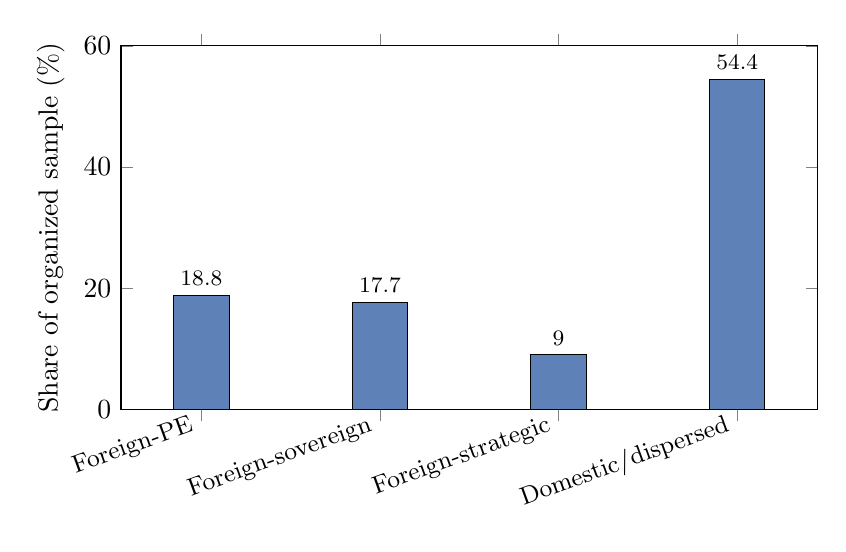
\begin{tikzpicture}
\begin{axis}[
  width=0.86\textwidth, height=6.2cm,
  ybar, bar width=20pt,
  ymin=0, ymax=60,
  ylabel={Share of organized sample (\%)},
  symbolic x coords={Foreign-PE,Foreign-sovereign,Foreign-strategic,Domestic/dispersed},
  xtick=data,
  x tick label style={rotate=20,anchor=east,font=\small},
  nodes near coords, nodes near coords style={font=\footnotesize},
  enlarge x limits=0.15,
]
\addplot[fill=secol!70] coordinates {(Foreign-PE,18.8) (Foreign-sovereign,17.7) (Foreign-strategic,9.0) (Domestic/dispersed,54.4)};
\end{axis}
\end{tikzpicture}
\caption{Foreign-capital control of the organized 14-chain hospital bed pool ($\sim$69{,}700 beds; share of sample). Foreign-PE (Blackstone$+$KKR) $+$ sovereign (Temasek) $=$ 36.6\%; all-foreign-controlled $=$ 45.6\%. \textit{Source:} 14-chain bed-ownership census, \cs{D:hospital\_bed\_ownership\_map}.}
\label{fig:ch1bedpool}
\end{figure}

% =====================================================================
\section{What Changed Since the June 2026 Baseline (Reader's Guide)}
% =====================================================================
For readers familiar with the baseline report, this edition adds or materially revises:

\begin{enumerate}[leftmargin=1.6em,itemsep=3pt]
\item \textbf{IHH $\rightarrow$ Fortis/Gleneagles} --- the largest foreign-control hospital position, absent from the baseline, now fully mapped (\S\ref{sec:hospitals}), including the Daiichi/Singh-brothers freeze and the November 2025 open-offer that drew near-zero acceptance (so IHH \emph{did not} reach majority).
\item \textbf{A bed-ownership concentration census} resolving the long-open ``25\% of organized beds'' claim (\S\ref{sec:concentration}).
\item \textbf{The ``PE-exited-via-IPO'' finding} --- Carlyle/Medanta, GA/KIMS, CDC-BII/Rainbow, KKR/Max --- which reframes the takeover narrative (\S\ref{sec:hospitals}).
\item \textbf{Single-specialty roll-ups and the GIC/AHH cross-vertical platform} (\S\ref{sec:singlespecialty}) --- the most concentrated arena of foreign-PE activity.
\item \textbf{A $\sim$60-transaction expansion} of the deal census across hospitals, single-specialty, pharma/CDMO, medtech, pharmacy, packaged food, quick commerce, agri-inputs, insurance and TPA (tables in \S\ref{sec:healthcare}--\S\ref{sec:food} and Appendix~C).
\item \textbf{Computed concentration (CR4/HHI)} for hospitals, diagnostics, packaged-food categories, health insurance and TPAs (\S\ref{sec:concentration}).
\item \textbf{A value-extraction scorecard} (global playbook vs documented India status) (\S\ref{sec:valueextraction}).
\item \textbf{The tax/treaty/GIFT-City structuring architecture} (\S\ref{sec:tax}).
\item \textbf{A documented influence/governance map} (IVCA, NATHEALTH, AdvaMed-GSP, electoral bonds) (\S\ref{sec:influence}).
\item \textbf{Deeper India-specific impact evidence} and \textbf{much deeper international comparators} (US: Steward, Envision, FTC-USAP; UK/Europe: Southern Cross, Four Seasons, Orpea; food: Kroger-Albertsons) (\S\ref{sec:indiaimpact}--\S\ref{sec:international}).
\item \textbf{A cross-cutting sovereign-wealth/pension lens} (\S\ref{sec:sovereign}) reframing the subject beyond ``US PE.''
\end{enumerate}

% =====================================================================
\section{Methodology and Evidence Standard}
% =====================================================================
\textbf{Two-layer method.} (1) Repository materials (generated reports, a PDF, charts) were treated as a \emph{claim inventory}, not as evidence; 71 recurring claims were separated and graded. (2) High-impact claims were tested against DPIIT/RBI/SEBI/IRDAI/CCI/NPPA/MoHFW/MoSPI/NABARD primary documents, BSE/NSE shareholding filings, company releases and prospectuses, CCI combination orders, peer-reviewed literature, and high-quality market-research (CRISIL, KPMG, Frost \& Sullivan, RedSeer, ICRA, Bain, EY). The June 2026 pass added 21 themed dossiers, each independently \emph{adversarially verified} by a second agent instructed to refute its load-bearing quantitative claims; refuted or unconfirmed claims were downgraded or dropped, and the dossiers' own self-corrections (e.g., ``Veeda is CX Partners, not CVC''; ``no QIA--Cloudnine link''; ``Savannah is RiceTec, not Bayer'') are carried into this report.

\textbf{Classification labels (used on every significant claim).} The five-level rubric is reproduced in the boxed legend in the front matter; in the body each significant claim is prefixed with its colour-coded small-caps label.

\textbf{Three discipline rules enforced throughout:} (i) ownership/control facts are kept separate from impact/causation claims; (ii) ``FPI \%'' category totals (from exchange filings) are facts about \emph{aggregate} foreign portfolio holding and never by themselves denote \emph{control} by any single owner; (iii) every concentration ratio states its denominator.

% =====================================================================
\section{Master Timeline (Updated)}
% =====================================================================
The most material verified events follow. \VF\ unless otherwise noted in the cell.

\begin{small}
\setlength{\tabcolsep}{4pt}
\begin{longtable}{>{\raggedright\arraybackslash}p{1.7cm} >{\raggedright\arraybackslash}p{13.5cm}}
\caption{Master timeline of material verified events. \textit{Sources:} as cited per row; see Appendix~A.}\label{tab:timeline}\\
\toprule
\textbf{Period} & \textbf{Evidence-based interpretation} \\
\midrule
\endfirsthead
\toprule
\textbf{Period} & \textbf{Evidence-based interpretation} \\
\midrule
\endhead
\midrule \multicolumn{2}{r}{\footnotesize\itshape continued on next page}\\
\endfoot
\bottomrule
\endlastfoot
1991--2000 & 1991 Statement on Industrial Policy liberalized FDI; \textbf{hospitals placed on the 100\% automatic route ($\sim$Jan 2000)} --- the most permanently open of all sectors here, meaning the FDI cap was \emph{never} the binding constraint on hospital deals \cs{S106}; \cs{D:fdi\_price\_control\_timeline}. \\
2005--2010 & Early foreign PE: Warburg Pincus $\rightarrow$ Max Healthcare (2005) \cs{S32}; Apax $\rightarrow$ Apollo (2007) \cs{S33}. DPIIT 2010 policy baseline \cs{S105}. \\
2011--2016 & \textbf{Policy counter-move and reversal in pharma:} Press Note 3/2011 moved \emph{brownfield} pharma to the approval route (takeover concern); PN1/2014 barred non-compete clauses; \textbf{PN5/2016 (24 Jun 2016) restored 74\% automatic} for brownfield. \textbf{Medical devices carved out to 100\% automatic} (Cabinet 26 Dec 2014; PN2/2015). \textbf{Food-product retail trading opened to 100\% FDI} (Budget 2016; operationalized 20 Jun 2016, Government route). \textbf{2016 tax-treaty pivot:} Mauritius (10 May 2016) and Singapore (Dec 2016) protocols $\rightarrow$ source-based capital-gains tax from 1 Apr 2017, with grandfathering \cs{D:tax\_treaty\_structuring}. \\
2017 & \textbf{NPPA price caps:} coronary stents (13 Feb 2017, $\sim$85\% cut) and knee implants (16 Aug 2017). GAAR effective (1 Apr 2017). Flagship corporate-hospital overcharging cases surface (Fortis Adya; Max Shalimar Bagh; Medanta) --- \emph{before} foreign control at those chains \cs{D:india\_impact\_evidence\_hunt}. \\
2018--2019 & \textbf{IHH acquires $\sim$31.1\% of Fortis (Nov 2018)} \cs{S158}; KKR-Radiant control of Max \cs{S146}; KKR exits Gland to Fosun \cs{S145}. Supreme Court freezes IHH's Fortis open offer (Dec 2018, Daiichi contempt). \textbf{AdvaMed$\rightarrow$USTR$\rightarrow$US withdraws India's GSP (5 Jun 2019)} over device price caps \cs{D:lobbying\_associations\_governance}. \\
2020--2022 & COVID-era private-hospital overcharging (82.5\% of audited episodes) \cs{D:india\_impact\_evidence\_hunt}. Carlyle$\rightarrow$Piramal Pharma (2020) \cs{S20}. \textbf{PE harvest cycle:} KKR exits Max ($\sim$US\$2bn, 2021--22); GA begins KIMS exit (IPO 2021); Carlyle exits Medanta (IPO 2022); CDC/BII exits Rainbow (IPO 2022). \textbf{Insurance FDI 49\%$\rightarrow$74\% (2021).} TPG/GIC build AHH; GIC enters (2022). \\
2023--2024 & \textbf{Temasek $\rightarrow$ Manipal ($\sim$59\%, Apr 2023)} \cs{S21}; Mubadala/Novo/CalPERS buy 8\% of Manipal (Feb 2024). \textbf{Blackstone/TPG build Quality Care; Aster--QCIL merger announced (Nov 2024)} \cs{S11}. Advent$\rightarrow$Suven control; Advent$\rightarrow$Apollo HealthCo/Keimed \cs{S101}; KKR$\rightarrow$Healthium \cs{S22}. \textbf{Temasek $+$ IHC $+$ Alpha Wave $\rightarrow$ Haldiram's ($\sim$16\% combined, $\sim$US\$10bn valuation, 2024--25)} \cs{S17}--\cs{S19}; \cs{D:sovereign\_institutional\_map}. \textbf{Finance (No.2) Act 2024:} LTCG 12.5\%, indexation removed, buyback-as-dividend (1 Oct 2024) \cs{D:tax\_treaty\_structuring}. \\
2025--2026 & \textbf{KKR $\rightarrow$ HCG control (54.27\%)} \cs{S13}; \cs{S104}; \textbf{Manipal buys Sahyadri from OTPP ($\sim$Rs 5{,}800 cr, Jul 2025)} \cs{D:sovereign\_institutional\_map}; Dr Agarwal's IPO (TPG/Temasek, Feb 2025); NephroPlus IPO (Quadria $\sim$30\%, Dec 2025); Sai Life --- TPG full exit (Aug 2025). \textbf{IHH's Fortis open offer finally runs (20 Oct--4 Nov 2025) but draws near-zero acceptance --- IHH stays at 31.17\%.} \textbf{Insurance FDI 74\%$\rightarrow$100\%} (Bill passed 17 Dec 2025; in force 5 Feb 2026) \cs{D:fdi\_price\_control\_timeline}. Quick-commerce ``Indianization'' (Eternal caps foreign at 49.5\%; Antfin exits; Zepto re-domiciles) \cs{D:quickcommerce\_delivery\_shares}. \\
\end{longtable}
\end{small}

% =====================================================================
\section{The Foreign-Capital Map --- Who, By Type}\label{sec:capitalmap}
% =====================================================================
The investigation's subject is best understood not as ``US PE'' but as five overlapping pools of foreign capital, each with a distinct risk profile (Figure~\ref{fig:dg1pools}):

\begin{enumerate}[leftmargin=1.6em,itemsep=3pt]
\item \textbf{US/European buyout PE} (control-seeking, 3--8yr exit cycles): Blackstone, KKR, Carlyle, Bain, TPG, Advent, General Atlantic, Warburg Pincus, CVC, Apax, EQT/BPEA, Bessemer, Goldman Sachs, ChrysCapital. \emph{Behaviour:} platform roll-ups, then IPO/secondary exit. Several flagship India hospital positions have already been \emph{fully exited} to public markets.
\item \textbf{Sovereign-wealth funds} (very long horizon, control \emph{or} minority): \textbf{Temasek} and \textbf{GIC} (Singapore --- the deepest), \textbf{ADIA}, \textbf{Mubadala}, \textbf{IHC} (Abu Dhabi), \textbf{QIA} (Qatar), \textbf{Khazanah} (Malaysia --- via IHH), \textbf{Saudi SALIC/PIF}. \emph{Behaviour:} anchor positions in defensive-growth assets; increasingly the \emph{consolidators}.
\item \textbf{Public pension plans:} \textbf{OTPP, CPPIB, CDPQ} (Canada), \textbf{CalPERS} (US), \textbf{CPP/Nuveen-TIAA}. \emph{Behaviour:} control exceptions (OTPP/Sahyadri) but mostly minority/credit; CalPERS leading Zepto is a notable direct startup bet.
\item \textbf{Development finance institutions (DFIs):} \textbf{IFC} (World Bank), \textbf{British International Investment} (UK), \textbf{ADB}, \textbf{FMO} (Netherlands), \textbf{IFU} (Denmark), \textbf{DFC} (US). \emph{Behaviour:} minority/impact capital; several have \emph{exited} (IFC/Agilus; CDC/Rainbow).
\item \textbf{Strategic multinationals (FDI, not financial PE):} \textbf{Mondelez} ($\sim$64\% of Indian chocolate), \textbf{PepsiCo} (via Varun Beverages), \textbf{Orkla} (MTR), \textbf{Hershey}, \textbf{McCain}, \textbf{Kirin} (Bira), \textbf{Viatris} (Biocon Biologics), \textbf{Mitsui} (via IHH). \emph{Behaviour:} outright control of the most profitable, highest-volume consumer categories.
\end{enumerate}

\VF\ (\emph{vehicle/jurisdiction pattern, where disclosed in CCI orders}). Post-2017 control stakes route predominantly through \textbf{Singapore Pte Ltd} vehicles (Temasek's Sheares/Jongsong; KKR's Tau/Hector; Blackstone's BCP Asia II Topco IV), consistent with the treaty pivot, while \textbf{Mauritius} SPVs persist for select sponsors (TPG's Centella Mauritius; Carlyle's CA Clover/CAP V Mauritius), and \textbf{Netherlands} (Warburg's South Elm; Morgan Stanley's NHPEA Sparkle) and \textbf{Cyprus} (Advent's Berhyanda) appear in specific deals \cs{D:tax\_treaty\_structuring}; \cs{D:medtech\_pharmacy\_distribution}.

% ---- FIGURE: DG1 five pools of foreign capital ----
\begin{figure}[htbp]
\centering
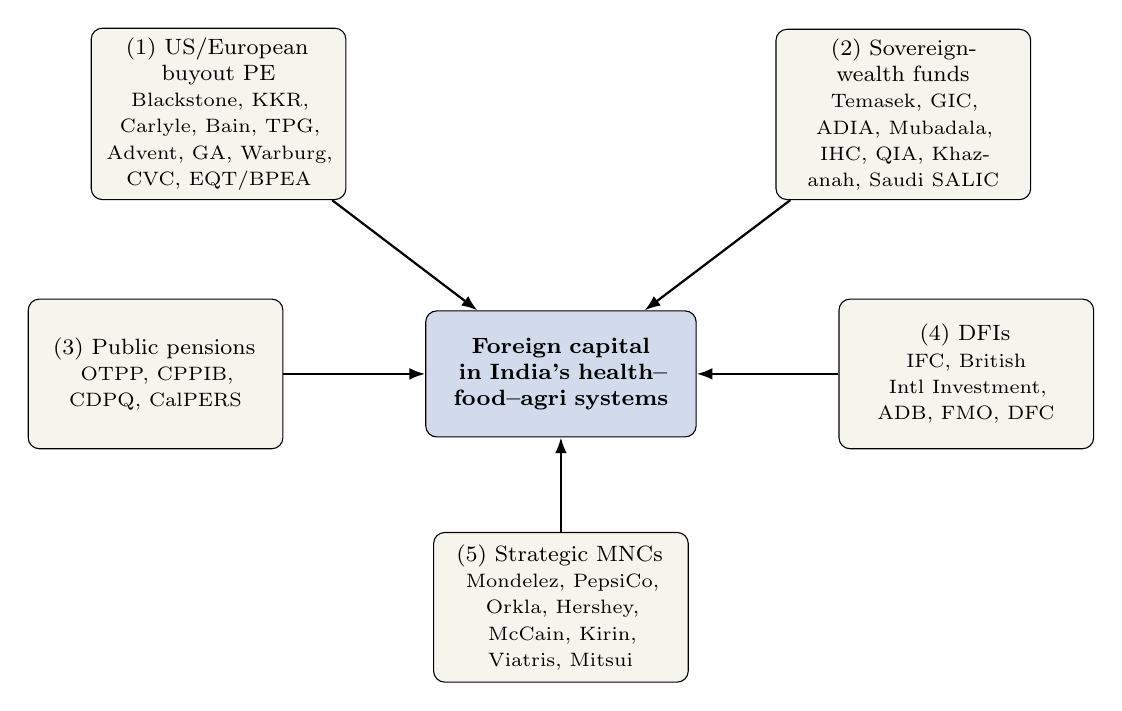
\begin{tikzpicture}[
  node distance=8mm and 6mm,
  every node/.style={font=\footnotesize},
  central/.style={rectangle, rounded corners, draw=black, fill=secol!20, align=center, text width=3.2cm, minimum height=1.6cm},
  pool/.style={rectangle, rounded corners, draw=black, fill=legendbg, align=center, text width=3.0cm, minimum height=1.9cm},
  arr/.style={-{Latex[length=2mm]}, thick}
]
\node[central] (c) {\textbf{Foreign capital in India's health--food--agri systems}};
\node[pool, above left=14mm and 10mm of c] (p1) {(1) US/European buyout PE\\ \scriptsize Blackstone, KKR, Carlyle, Bain, TPG, Advent, GA, Warburg, CVC, EQT/BPEA};
\node[pool, above right=14mm and 10mm of c] (p2) {(2) Sovereign-wealth funds\\ \scriptsize Temasek, GIC, ADIA, Mubadala, IHC, QIA, Khazanah, Saudi SALIC};
\node[pool, left=18mm of c] (p3) {(3) Public pensions\\ \scriptsize OTPP, CPPIB, CDPQ, CalPERS};
\node[pool, right=18mm of c] (p4) {(4) DFIs\\ \scriptsize IFC, British Intl Investment, ADB, FMO, DFC};
\node[pool, below=12mm of c] (p5) {(5) Strategic MNCs\\ \scriptsize Mondelez, PepsiCo, Orkla, Hershey, McCain, Kirin, Viatris, Mitsui};
\draw[arr] (p1) -- (c);
\draw[arr] (p2) -- (c);
\draw[arr] (p3) -- (c);
\draw[arr] (p4) -- (c);
\draw[arr] (p5) -- (c);
\end{tikzpicture}
\caption{The five pools of foreign capital in India's health--food--agri systems. \textit{Source:} synthesis, \cs{D:sovereign\_institutional\_map}; \cs{D:tax\_treaty\_structuring}.}
\label{fig:dg1pools}
\end{figure}

% =====================================================================
\section{Cross-Cutting Finding: Sovereign and Pension Capital is the Centre of Gravity}\label{sec:sovereign}
% =====================================================================
\SE\ A small cluster of foreign government-linked funds now sits at or near the top of India's largest private hospital and branded-food assets \cs{D:sovereign\_institutional\_map}:

\begin{itemize}[leftmargin=1.4em,itemsep=3pt]
\item \textbf{Temasek (Singapore)} --- the deepest single position. \emph{Control:} Manipal ($\sim$59\%, \#2 chain) and, via Manipal, Sahyadri. \emph{Significant minority:} Medanta ($\sim$17\%, via Dunearn Mauritius), Dr Agarwal's ($\sim$28\% pre-IPO), Cloudnine ($\sim$18--20\%, reported), Haldiram's ($\sim$10\%), plus Country Delight, Licious, Rebel Foods, Devyani, and historically Intas (10.16\%, 2014). Temasek's India head stated (Jul 2024) intent to deploy up to \textbf{US\$10bn more in India over three years}, naming healthcare a theme.
\item \textbf{GIC (Singapore)} --- controls/anchors \textbf{Asia Healthcare Holdings} (US\$320m), spanning Nova IVF, Motherhood and AINU; Rainbow IPO anchor.
\item \textbf{Khazanah (Malaysia)} --- largest bloc behind \textbf{IHH} $\rightarrow$ strategic owner of \textbf{Fortis} ($\sim$31\%) and \textbf{Gleneagles}; separately $\sim$15\% of \textbf{Wow! Momo}.
\item \textbf{Abu Dhabi cluster (ADIA, Mubadala, IHC)} --- ADIA in Rainbow, Sapphire Foods, \textbf{Meril} (medtech, $\sim$3\%, EV $\sim$US\$6.6bn) and \textbf{Aditya Birla Health} (10\%); Mubadala in Manipal; IHC $+$ Alpha Wave in Haldiram's ($\sim$6\%) and \textbf{Advanta} seeds ($\sim$12.5\%).
\item \textbf{Canadian pensions} --- \textbf{OTPP} controlled \textbf{Sahyadri} (first India control buyout, 2022) then exited to Temasek/Manipal in 2025 at $\sim$2.5x; \textbf{CPPIB/CDPQ} mostly minority/credit (CDPQ's US\$300m private-credit platform with Piramal).
\item \textbf{CalPERS (US)} --- Manipal co-investor (8\% consortium, 2024) and \textbf{lead of Zepto's $\sim$US\$450m round} (2025) at US\$7bn.
\item \textbf{Saudi SALIC (PIF)} --- $\sim$9.22\% of listed \textbf{LT Foods} (Daawat basmati), 2025.
\end{itemize}

\EI\ Singapore state capital alone (Temasek $+$ GIC) touches India's \#2 hospital chain, a leading single-specialty platform, pediatric care, and the \#1 branded-snacks company. The clearest consolidation vector is sovereign-to-sovereign/pension: OTPP's Sahyadri folding into Temasek's Manipal shows capital not merely buying assets but \textbf{rolling up regional chains under a single foreign-government-controlled platform}. This reframes the policy question: the relevant actor class is \emph{foreign institutional and sovereign capital}, of which US buyout PE is one --- and increasingly not the dominant --- component. The sovereign/pension footprint is mapped compactly in Figure~\ref{fig:dg4footprint}.

% =====================================================================
\section{Healthcare Sector Findings}\label{sec:healthcare}
% =====================================================================
\subsection{Hospitals}\label{sec:hospitals}

\textbf{(a) IHH $\rightarrow$ Fortis / Gleneagles --- the largest foreign-control position (new).}

\VF\ \textbf{IHH Healthcare Berhad} (Bursa/SGX-listed; ultimate holders Mitsui $\sim$32.7\%, Khazanah $\sim$26\%, Malaysia's EPF $\sim$11--13\%) is the \textbf{classified promoter of Fortis Healthcare with 31.17\%} (235{,}295{,}895 shares) --- the single largest block, with no other promoter and a dispersed float, conferring effective working control \cs{S158}; \cs{S159}; \cs{D:ihh\_fortis\_gleneagles}. IHH entered via a \textbf{November 2018 preferential allotment ($\sim$Rs 4{,}000 cr at Rs 170/share, $\sim$31.1\%)} through the Singapore SPV \textbf{Northern TK Venture}, winning a 2018 bidding war against TPG-Manipal, the Hero--Burman consortium, KKR-Radiant and China's Fosun. The control chain is mapped in Figure~\ref{fig:dg2ihh}.

\VF\ (\emph{decisive 2025 development}). IHH's mandatory \textbf{26.1\% open offer was frozen for $\sim$7 years} by a Supreme Court status-quo order arising from Daiichi Sankyo's contempt action against Fortis's former promoters, the \textbf{Singh brothers} (rooted in the 2008 Ranbaxy sale to Daiichi and the Religare/RHC fund-diversion case). SEBI cleared the offer in October 2025; it ran 20 Oct--4 Nov 2025 at Rs 170 $+$ Rs 53.80 interest. \textbf{It drew near-zero acceptance (1{,}778 shares, 0.0002\%)} because Fortis traded $\sim$Rs 980 --- six times the offer price. \textbf{IHH therefore remained at 31.17\% and did NOT reach majority.} Press headlines that ``IHH committed to raise its stake to 50\%'' describe \emph{intent}, not an executed majority --- a \PH\ / forward statement, not a fact \cs{S158}; \cs{S160}; \cs{D:ihh\_fortis\_gleneagles}.

\VF\ IHH separately owns \textbf{100\% of Gleneagles Healthcare India} ($\sim$1{,}200--1{,}500 beds; 100\% reached via a $\sim$Rs 740 cr 2023 buyout) and $\sim$62.7\% of listed Fortis Malar; from July 2025 Fortis operates five Gleneagles hospitals under an O\&M agreement. The combined IHH-India network is reported at \textbf{$\sim$35 hospitals, $>$5{,}000 beds across 11 states}, targeting $\sim$7{,}000 by 2028. Fortis's diagnostics arm \textbf{Agilus (ex-SRL)} was taken from 57.68\% toward 100\% by buying out PE holders \textbf{IFC, NYLIM Jacob Ballas and Avigo} (CCI-cleared Oct 2024) --- a \emph{reverse} flow in which development/India PE exited a large diagnostics chain into the IHH-controlled umbrella \cs{S161}; \cs{S162}; \cs{D:ihh\_fortis\_gleneagles}.

% ---- FIGURE: DG2 IHH control chain ----
\begin{figure}[htbp]
\centering
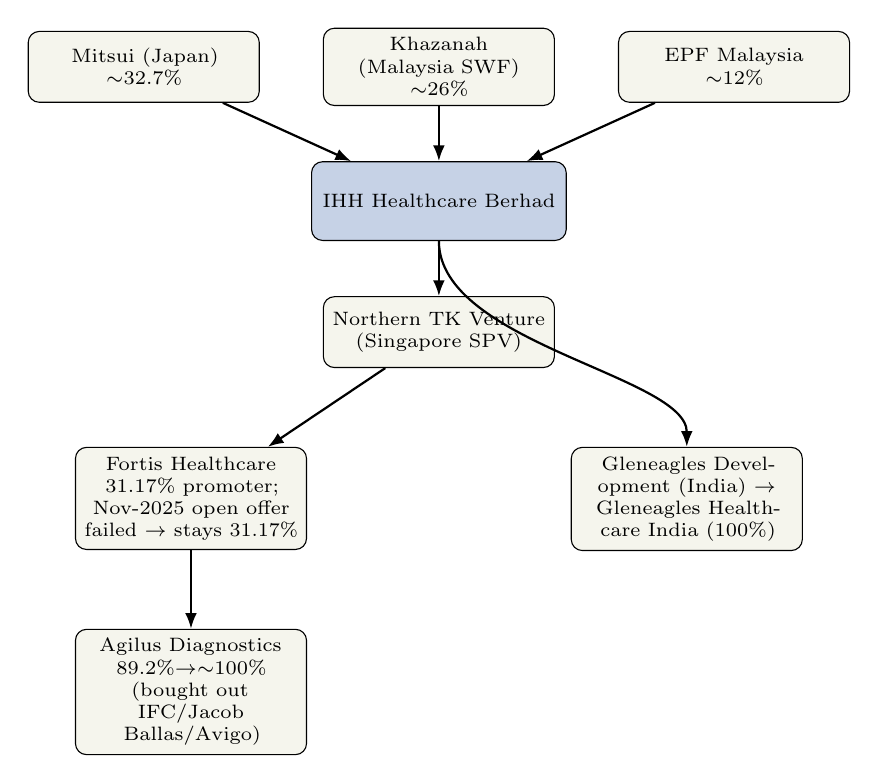
\begin{tikzpicture}[
  every node/.style={font=\scriptsize},
  box/.style={rectangle, rounded corners, draw=black, fill=legendbg, align=center, text width=2.7cm, minimum height=0.9cm},
  hub/.style={rectangle, rounded corners, draw=black, fill=secol!25, align=center, text width=3.0cm, minimum height=1.0cm},
  arr/.style={-{Latex[length=2mm]}, thick},
  node distance=7mm and 8mm
]
\node[box] (mitsui) {Mitsui (Japan)\\ $\sim$32.7\%};
\node[box, right=of mitsui] (khaz) {Khazanah (Malaysia SWF)\\ $\sim$26\%};
\node[box, right=of khaz] (epf) {EPF Malaysia\\ $\sim$12\%};
\node[hub, below=of khaz] (ihh) {IHH Healthcare Berhad};
\node[box, below=of ihh] (ntk) {Northern TK Venture (Singapore SPV)};
\node[box, below left=10mm and 2mm of ntk] (fortis) {Fortis Healthcare\\ 31.17\% promoter; Nov-2025 open offer failed $\rightarrow$ stays 31.17\%};
\node[box, below right=10mm and 2mm of ntk] (glen) {Gleneagles Development (India) $\rightarrow$ Gleneagles Healthcare India (100\%)};
\node[box, below=10mm of fortis] (agilus) {Agilus Diagnostics 89.2\%$\rightarrow$$\sim$100\% (bought out IFC/Jacob Ballas/Avigo)};
\draw[arr] (mitsui) -- (ihh);
\draw[arr] (khaz) -- (ihh);
\draw[arr] (epf) -- (ihh);
\draw[arr] (ihh) -- (ntk);
\draw[arr] (ntk) -- (fortis);
\draw[arr] (ihh.south) .. controls +(0,-1.3) and +(0,0.9) .. (glen.north);
\draw[arr] (fortis) -- (agilus);
\end{tikzpicture}
\caption{IHH $\rightarrow$ Fortis / Gleneagles control chain. \textit{Source:} \cs{S158}--\cs{S162}; \cs{D:ihh\_fortis\_gleneagles}.}
\label{fig:dg2ihh}
\end{figure}

\textbf{(b) Temasek/Manipal, Blackstone/Aster-QCIL, KKR/HCG (verified controls).}

\VF\ \textbf{Temasek-linked entities became the dominant shareholder of Manipal} after 2023 (Temasek $+$41\%; Sheares 18\%; TPG 11\%; Manipal Group $\sim$30\%; NIIF fully exited); Manipal's 2026 SEBI prospectus shows \textbf{48 hospitals and 12{,}367 licensed beds} (Sep 30, 2025) and pre-offer promoters of 69.86\% \cs{S21}; \cs{S117}. In \textbf{July 2025 Manipal bought Sahyadri from OTPP ($\sim$Rs 5{,}800 cr)}, taking it to 49 hospitals \cs{D:sovereign\_institutional\_map}.

\VF\ \textbf{Blackstone- and TPG-backed Quality Care India} (CARE/KIMS Health/Evercare; QCIL promoter block BCP Asia II Topco IV at 71.84\% \cs{S119}) received CCI approval to merge into \textbf{Aster DM Healthcare} (combined $\sim$38 hospitals, 10{,}150$+$ beds; announced post-merger Blackstone $\sim$30.7\%, Aster promoters $\sim$24.0\%, joint control) \cs{S10}; \cs{S11}; NCLT sanction was pending as of mid-2026 \cs{S118}. CCI's order named Blackstone's Singapore and TPG's Mauritius (Centella) vehicles \cs{D:tax\_treaty\_structuring}.

\VF\ \textbf{KKR} controls \textbf{HCG} (Hector Asia Holdings II, 54.27\%; total promoter group 64.21\% per March 2026 BSE) \cs{S13}; \cs{S104}, acquired from \textbf{CVC} for up to $\sim$US\$400m, with stated sole operational control; KKR also controls \textbf{Healthium MedTech} (from Apax, $\sim$US\$839m press-reported) \cs{S22} and acquired \textbf{Baby Memorial Hospital} (2024) \cs{S24}.

\textbf{(c) The ``PE-exited-via-IPO'' finding (new, narrative-correcting).}

\VF\ Several marquee US-buyout-PE hospital positions have been \emph{fully harvested}, leaving Indian founders and diffuse FPI in control \cs{D:hospital\_chains\_pe\_census}:
\begin{itemize}[leftmargin=1.4em,itemsep=2pt]
\item \textbf{Carlyle} entered Medanta/Global Health (2013, $\sim$25.67\%) and \textbf{fully exited at the November 2022 IPO}; Temasek retains $\sim$17\% (via Mauritius); founder Dr Trehan $\sim$33\%.
\item \textbf{General Atlantic} invested Rs 929 cr for 38.99\% of \textbf{KIMS Hyderabad} (2018) and \textbf{fully exited ($\sim$3.58x) by 2024} via IPO and blocks; founder Bollineni family controls $\sim$34\%.
\item \textbf{UK's CDC/British International Investment} backed \textbf{Rainbow Children's} and \textbf{fully exited at the 2022 IPO}; ADIA ($\sim$2\%) is a passive FPI; founder Kancharla family $\sim$50\%.
\item \textbf{KKR} built \textbf{Max Healthcare} (via Radiant, 2018) and \textbf{fully exited 2021--22} ($\sim$US\$2bn, PE's largest India exit, buyers incl. GIC/MAS); promoter Abhay Soi $\sim$24\%, FPIs $\sim$45\% (March 2026 BSE) \cs{S108}.
\end{itemize}

\EI\ This materially qualifies the ``foreign takeover'' thesis. Foreign buyout PE has frequently \emph{cycled through} Indian hospital assets (build $\rightarrow$ list $\rightarrow$ exit), converting concentrated PE stakes into dispersed public/FPI float under Indian-founder or sovereign control. The durable foreign-\emph{control} positions are the strategic/sovereign ones (IHH, Temasek, KKR/HCG, Blackstone-incoming), not a uniform PE ownership of the sector.

\textbf{(d) The bed-ownership map and the concentration paradox.} See \S\ref{sec:concentration} for the consolidated 14-chain bed census and the resolution of the ``25\% of organized beds'' claim.

\subsection{Single-Specialty Roll-Ups --- the Most Concentrated Arena}\label{sec:singlespecialty}

\SE\ Single-specialty verticals (eye, IVF, dialysis, oncology, mother \& child, nephro-urology) are where foreign-PE/sovereign/DFI capital is \emph{most} concentrated, because asset-light, replicable clinical units are ideal roll-up targets \cs{D:single\_specialty\_rollups}:

\begin{itemize}[leftmargin=1.4em,itemsep=2pt]
\item \textbf{Eye care:} \textbf{Dr Agarwal's} (TPG $\sim$33.75\% $+$ Temasek $\sim$28.18\% pre-IPO; IPO Feb 2025, $\sim$Rs 3{,}027 cr) \cs{S171}; \textbf{ASG Eye} (General Atlantic $+$ Kedaara, Rs 1{,}500 cr/2022, after an Investcorp exit) \cs{S170}; \textbf{Centre for Sight} (ChrysCapital, up to US\$100m/2024, ex-Mahindra); \textbf{Maxivision} (Quadria, up to Rs 1{,}300 cr/2023).
\item \textbf{Fertility/IVF:} \textbf{Indira IVF} (BPEA EQT majority/control 2023, press $\sim$60\%/$\sim$Rs 6{,}000 cr at $\sim$US\$1.1bn; ex-TA Associates) \cs{S169}; \textbf{Nova IVF} (inside AHH/GIC); \textbf{Ferty9} (Verlinvest control, US\$50m/2023); \textbf{Oasis} (Kedaara minority).
\item \textbf{Dialysis:} \textbf{NephroPlus} (Asia's largest; Quadria $\sim$30\% largest holder; IPO Dec 2025; ex-Investcorp/Bessemer/IFC/IIFL) \cs{S172}; \textbf{DCDC} (BII/ADB/IFU/Temasek-backed ABC Impact).
\item \textbf{Oncology:} \textbf{HCG} (CVC$\rightarrow$KKR 2025); \textbf{AOI/CTSI} (TPG$\rightarrow$Varian$\rightarrow$Siemens --- now \emph{strategic}, not PE).
\item \textbf{Mother \& child:} \textbf{Cloudnine} (Temasek $+$ TPG NewQuest $\sim$52\%; a $\sim$25\%/Rs 11{,}000 cr stake sale process drew TPG/Advent/CVC/Permira in 2026); \textbf{Motherhood} (AHH).
\item \textbf{Nephro-urology:} \textbf{AINU} (AHH, $>$70\%/Rs 600 cr/2023).
\end{itemize}

\SE\ (\emph{the headline structural fact}). A \textbf{single Singapore-sovereign-controlled holding company --- Asia Healthcare Holdings (GIC, co-invested TPG)} --- spans IVF (Nova, $\sim$95 centres/57 cities), mother \& child (Motherhood, $\sim$24 hospitals/12 cities) and nephro-urology (AINU, 7 hospitals/500$+$ beds). This \emph{cross-vertical concentration under one foreign controller} is the single most antitrust-relevant datapoint in the healthcare-services census, even though no CCI order has yet quantified market shares in these verticals \cs{S153}; \cs{S157}; \cs{D:single\_specialty\_rollups}. The platform is depicted in Figure~\ref{fig:dg3ahh}.

% ---- FIGURE: DG3 AHH platform ----
\begin{figure}[htbp]
\centering
\begin{tikzpicture}[
  every node/.style={font=\scriptsize},
  box/.style={rectangle, rounded corners, draw=black, fill=legendbg, align=center, text width=3.0cm, minimum height=1.0cm},
  hub/.style={rectangle, rounded corners, draw=black, fill=secol!25, align=center, text width=3.4cm, minimum height=1.0cm},
  top/.style={rectangle, rounded corners, draw=black, fill=vfcol!18, align=center, text width=3.4cm, minimum height=0.9cm},
  arr/.style={-{Latex[length=2mm]}, thick},
  node distance=9mm and 10mm
]
\node[top] (gic) {GIC (Singapore SWF) $+$ TPG};
\node[hub, below=of gic] (ahh) {Asia Healthcare Holdings (US\$320m)};
\node[box, below left=10mm and 6mm of ahh] (nova) {Nova IVF\\ 95 centres, 57 cities};
\node[box, below=10mm of ahh] (mother) {Motherhood\\ 24 hospitals, 12 cities};
\node[box, below right=10mm and 6mm of ahh] (ainu) {AINU\\ 7 hospitals, nephro-urology};
\draw[arr] (gic) -- (ahh);
\draw[arr] (ahh) -- (nova);
\draw[arr] (ahh) -- (mother);
\draw[arr] (ahh) -- (ainu);
\end{tikzpicture}
\caption{GIC / Asia Healthcare Holdings single-specialty platform: one sovereign-controlled holding company spans three single-specialty verticals. \textit{Source:} \cs{S153}; \cs{S157}; \cs{D:single\_specialty\_rollups}.}
\label{fig:dg3ahh}
\end{figure}

% ---- FIGURE: DG4 sovereign/pension footprint (styled table inside figure) ----
\begin{figure}[htbp]
\centering
\small
\setlength{\tabcolsep}{6pt}
\fcolorbox{black}{white}{%
\begin{minipage}{0.95\textwidth}
\centering\textbf{Sovereign / Pension Footprint Map}\par\vspace{4pt}
\begin{tabularx}{\textwidth}{@{}l>{\raggedright\arraybackslash}X@{}}
\toprule
\textbf{Fund} & \textbf{Indian footprint} \\
\midrule
Temasek (SG) & Manipal ($\sim$59\% control), Sahyadri (via Manipal), Medanta $\sim$17\%, Dr Agarwal's $\sim$28\%, Cloudnine, Haldiram's $\sim$10\%, Licious, Country Delight \\
GIC (SG) & Asia Healthcare Holdings (control) \\
Khazanah (MY) & IHH/Fortis, Wow! Momo $\sim$15\% \\
ADIA (UAE) & Rainbow, Meril $\sim$3\%, Aditya Birla Health 10\% \\
Mubadala (UAE) & Manipal (8\% consortium) \\
OTPP (CA) & Sahyadri (control, exited to Manipal) \\
CalPERS (US) & Zepto (lead), Manipal \\
Saudi SALIC & LT Foods $\sim$9.2\% \\
\bottomrule
\end{tabularx}
\end{minipage}}
\caption{Sovereign / pension footprint across India's health and food assets. \textit{Source:} \cs{S226}; \cs{D:sovereign\_institutional\_map}.}
\label{fig:dg4footprint}
\end{figure}

\subsection{Diagnostics}

\VF\ Foreign capital is pervasive across diagnostics but the market is genuinely fragmented. Historical/current positions: \textbf{Carlyle} entered Metropolis (2015) and \textbf{exited 2024} ($\sim$US\$99m, 13\%); \textbf{WestBridge} in Dr Lal; \textbf{API/PharmEasy} controls Thyrocare (66\%$+$, $\sim$US\$613m/2021) \cs{S35}; \textbf{Fortis} consolidated \textbf{Agilus} to $\sim$96\%$+$ by buying out IFC/Jacob Ballas/Avigo \cs{S111}; \cs{D:ihh\_fortis\_gleneagles}; \textbf{OrbiMed} (Mauritius) $\sim$19.5\% of Suraksha (East India); \textbf{Kedaara} $\sim$10\% of Vijaya. Current listed cap tables (March 2026 BSE) show \textbf{no current single PE controller} of Dr Lal (promoter 53.21\%) or Metropolis (promoter 48.87\%) \cs{S109}; \cs{S110}.

\SE\ (\emph{concentration}). Per CRISIL primary reports, \textbf{diagnostic chains are only $\sim$20--24\% of the $\sim$Rs 1{,}000--1{,}070bn total diagnostics market} (FY24, up from 13--17\% in FY20); within that, even the leader \textbf{Dr Lal holds just 5.3--5.7\% of its strongest region (North)}, Metropolis 2.5--2.8\% (West), Vijaya 2.2--2.5\% (South). CR4 of the \emph{chains} pool $\approx$ 24--30\%; CR5 of the \emph{total} market $\approx$ 6--7\%. The story is \textbf{rapid consolidation momentum and foreign-PE backing of the consolidators, not present-day dominance} \cs{S163}; \cs{S164}; \cs{D:concentration\_hospitals\_diagnostics}. See Figure~\ref{fig:ch10diag}.

% ---- FIGURE: CH10 diagnostic chains share of total ----
\begin{figure}[htbp]
\centering
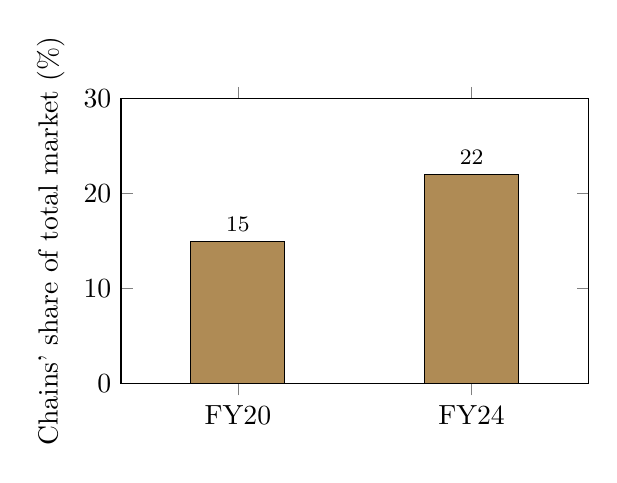
\begin{tikzpicture}
\begin{axis}[
  width=0.62\textwidth, height=5.2cm,
  ybar, bar width=34pt,
  ymin=0, ymax=30,
  ylabel={Chains' share of total market (\%)},
  symbolic x coords={FY20,FY24},
  xtick=data,
  nodes near coords, nodes near coords style={font=\footnotesize},
  enlarge x limits=0.5,
]
\addplot[fill=eicol!70] coordinates {(FY20,15) (FY24,22)};
\end{axis}
\end{tikzpicture}
\caption{Diagnostic chains' share of India's total diagnostics market (\%). FY20 $\sim$15\% (mid 13--17); FY24 $\sim$22\% (mid 20--24). Leader Dr Lal holds $<$6\% nationally. \textit{Source:} CRISIL, \cs{S164}; \cs{D:concentration\_hospitals\_diagnostics}.}
\label{fig:ch10diag}
\end{figure}

\subsection{Pharmaceuticals, CDMO and CRO}

\SE\ The pharma-services stack (APIs, CDMO/CRDMO, CRO) is the most foreign-\emph{controlled} life-sciences segment, because buyout funds favour the export-oriented, dollar-revenue services model \cs{D:pharma\_pe\_census}:
\begin{itemize}[leftmargin=1.4em,itemsep=2pt]
\item \textbf{Foreign-controlled CDMO/CRO:} \textbf{Advent (US)} built \textbf{Cohance Lifesciences} (RA Chem/ZCL/Avra) and acquired control of listed \textbf{Suven Pharmaceuticals} (50.1\% at Rs 495/share, then $\sim$76.1\%; CCEA-approved FDI up to Rs 9{,}589 cr via Cyprus vehicle \textbf{Berhyanda}), merging the two in 2025 \cs{S174}; \textbf{TPG (US)} controlled \textbf{Sai Life Sciences} (2018; $\sim$39\% pre-IPO via Singapore vehicle) and \textbf{fully exited Aug 2025} \cs{S175}; \textbf{PAG} built the \textbf{Sekhmet} API platform (Singapore holdco; Optimus, Anjan).
\item \textbf{Large foreign \emph{minorities} in founder-controlled pharma:} \textbf{ChrysCapital $+$ Temasek} in \textbf{Intas} (Temasek 10.16\% from 2014) \cs{S177}; \textbf{ChrysCapital $+$ Capital International} pre-IPO in \textbf{Mankind} (largely exited at 2023 IPO); \textbf{Goldman Sachs ($\sim$one-third) $+$ Quadria ($\sim$10\%)} in \textbf{Aragen} (ex-GVK Bio) \cs{S176}; \textbf{Goldman, ADQ, Viatris ($\ge$12.9\%)} in \textbf{Biocon Biologics} \cs{S178}; \textbf{Carlyle} $\sim$18\% of \textbf{Piramal Pharma} (Mauritius vehicle, gradually exiting) \cs{S20}.
\item \textbf{Exited/dispersed:} \textbf{Warburg Pincus} exited Laurus Labs; \textbf{ChrysCapital} exited Eris (2024); \textbf{Bain} holds Emcure (ex-Blackstone, 2013) \cs{S144}.
\end{itemize}

\VF\ CCI's \textbf{Torrent--JB Chemicals} order (KKR's exit) shows competition review \emph{can} reach product-level overlaps: CCI found prima facie AAEC in specific finished-dosage-form markets and approved only after remedies (Vizylac licensing; Calcigard divestiture; Azovas price cap) \cs{S15}. The pharma story is therefore \emph{not} simple foreign control: it includes PE exits to Indian strategics (BSV$\rightarrow$Mankind \cs{S23}; Gland$\rightarrow$Fosun \cs{S145}), founder-retained control, and granular CCI scrutiny.

\subsection{Medical Devices and Pharmacy/Distribution}

\SE\ Medical devices are mostly \textbf{founder-controlled with foreign minorities}, with one clean foreign-PE \emph{control} case \cs{D:medtech\_pharmacy\_distribution}:
\begin{itemize}[leftmargin=1.4em,itemsep=2pt]
\item \textbf{Meril} (Bilakhia family) --- Warburg Pincus $\sim$13\% (Netherlands vehicle) $+$ \textbf{ADIA $\sim$3\% (2025, EV $\sim$US\$6.6bn)} \cs{S179}; \textbf{SMT} stents (Samara $+$ Morgan Stanley PE $\sim$18\% jointly $>$55\%; IPO-bound) \cs{S180}; \textbf{Poly Medicure, Trivitron} --- passive/declining FPI; \textbf{Healthium} --- the clean control case (\textbf{Apax $\rightarrow$ KKR}, $\sim$US\$839m/2024) \cs{S181}.
\item \textbf{Pharmacy/distribution} splits sharply by control: market \emph{leaders are domestic} --- \textbf{Tata 1mg} (\#1 e-pharmacy by GMV, $\sim$31\%) \cs{S183} and \textbf{Apollo Pharmacy} (\#1 retail, $\sim$7{,}000 stores) --- while the most foreign-capital-intensive player, \textbf{PharmEasy/API Holdings} (Prosus/TPG/Temasek/CDPQ), \textbf{lost $\sim$92\% of its peak US\$5.6bn value} and ceded leadership \cs{S184}. \textbf{Advent (12.1\%)} co-invested the \textbf{Apollo HealthCo $+$ Keimed} merger (fusing India's \#1 retail pharmacy with its leading wholesale distributor; AHEL retains $\ge$59.2\%) \cs{S101}. \textbf{Warburg Pincus fully exited MedPlus in 2024} (to GIC/ICICI Pru) \cs{S185}. \emph{Net:} heavy foreign capital, but durable control of the pharmacy/distribution leaders is \textbf{domestic}.
\end{itemize}

\subsection{Insurance and Third-Party Administrators (TPAs)}

\SE\ (\emph{the value-chain gradient}). Concentration and foreign-capital intensity \emph{rise} as one moves from insurers to the claims-administration layer \cs{D:concentration\_food\_insurance\_tpa} (Figure~\ref{fig:dg5gradient}):
\begin{itemize}[leftmargin=1.4em,itemsep=2pt]
\item \textbf{Overall health insurance is NOT concentrated:} HHI $\approx$ 700--830; CR4 $\approx$ 43.5\% (largest $=$ public New India $\sim$17\%). Foreign JV partners sit at the \emph{insurer} level: \textbf{Bupa ($\sim$63\% of Niva Bupa)}, \textbf{Cigna (49\% of ManipalCigna)}, \textbf{ADIA (10\% of Aditya Birla Health)}, \textbf{Allianz} (exiting Bajaj Allianz) \cs{S188}. Insurance FDI rose 26$\rightarrow$49$\rightarrow$74$\rightarrow$\textbf{100\% (in force Feb 2026)}.
\item \textbf{Retail health is moderately concentrated:} Star $+$ Care $+$ Niva Bupa $\approx$ 52\% (SAHIs $\sim$56\%); \textbf{Star Health} (WestBridge/Safecrop consortium) leads retail ($\sim$33\%) \cs{S186}.
\item \textbf{The TPA claims layer is highly concentrated and most foreign-capital-linked:} CR4 $\approx$ 68\% (premium serviced); \textbf{Medi Assist} alone $\sim$31\% (rising to $\sim$37\% of group premium after acquiring \textbf{Paramount} from Canada's Fairfax in 2024), and TPAs process $\sim$76\% of claims by volume. Medi Assist was \textbf{built on Bessemer (US) $\sim$45\% and Investcorp (Gulf) $\sim$21\%}, partly sold down at its 2024 IPO (some to Denmark's Novo Holdings) \cs{S48}; \cs{S112}; \cs{S187}.
\end{itemize}

\PH\ Because the TPA layer adjudicates $\sim$76\% of claims and is now dominated by a single foreign-PE-incubated player, ownership incentives \emph{could} affect claim approval, network bargaining and settlement deductions --- but no evidence proves ownership-caused denials. IRDAI FY25 data show insurers settled 87\% of health-claim counts (8\% repudiated) with 69\% routed through TPAs \cs{S79}. This is the highest-priority insurance/TPA monitoring target.

% ---- FIGURE: DG5 concentration vs foreign-capital gradient ----
\begin{figure}[htbp]
\centering
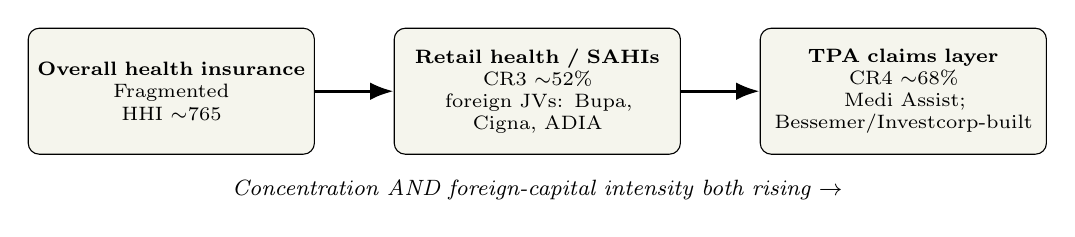
\begin{tikzpicture}[
  every node/.style={font=\scriptsize},
  stg/.style={rectangle, rounded corners, draw=black, fill=legendbg, align=center, text width=3.4cm, minimum height=1.6cm},
  arr/.style={-{Latex[length=3mm]}, very thick},
  node distance=10mm
]
\node[stg] (a) {\textbf{Overall health insurance}\\ Fragmented\\ HHI $\sim$765};
\node[stg, right=of a] (b) {\textbf{Retail health / SAHIs}\\ CR3 $\sim$52\%\\ foreign JVs: Bupa, Cigna, ADIA};
\node[stg, right=of b] (c) {\textbf{TPA claims layer}\\ CR4 $\sim$68\%\\ Medi Assist; Bessemer/Investcorp-built};
\draw[arr] (a) -- (b);
\draw[arr] (b) -- (c);
\node[below=2mm of b, font=\footnotesize\itshape] {Concentration AND foreign-capital intensity both rising $\rightarrow$};
\end{tikzpicture}
\caption{Concentration vs foreign-capital intensity gradient down the health-financing value chain. \textit{Source:} \cs{D:concentration\_food\_insurance\_tpa}; \cs{S79}; \cs{S186}--\cs{S188}.}
\label{fig:dg5gradient}
\end{figure}

\subsection{Digital Health}

\VF\ Foreign-PE exposure extends into healthcare RCM and platform health: \textbf{KKR $+$ Norwest $\rightarrow$ Infinx} (AI revenue-cycle management) \cs{S100}; \textbf{Advent $\rightarrow$ Apollo HealthCo/24$|$7} \cs{S101}; \textbf{EQT/BPEA $\rightarrow$ Sagility} (US-healthcare BPO, IPO 2024) \cs{S149}; \cs{S156}; \textbf{New Mountain Capital $\rightarrow$ Access Healthcare} ($\sim$US\$1.5bn, 2025) \cs{D:value\_extraction\_india\_hospitals}. India-facing platforms (Tata 1mg, Apollo 24$|$7) remain domestically controlled; the offshore-facing BPO/RCM tier is institutionally controlled.

% =====================================================================
\section{Food, Agriculture and Nutrition Findings}\label{sec:food}
% =====================================================================
\subsection{Packaged Food / FMCG / Beverages}

\VF\ Foreign institutional, sovereign, family-office and strategic-MNC capital is pervasive across packaged food, and it has \textbf{disproportionately scaled the HFSS/UPF categories} \cs{D:packaged\_food\_pe\_census}:
\begin{itemize}[leftmargin=1.4em,itemsep=2pt]
\item \textbf{Snacks (UPF):} Haldiram Snacks Food --- \textbf{Temasek $\sim$10\%, IHC$+$Alpha Wave $\sim$6\%} at a $\sim$US\$10bn valuation (2024--25) \cs{S17}--\cs{S19}; \cs{D:sovereign\_institutional\_map}; Balaji Wafers --- \textbf{General Atlantic 6.93\%} \cs{S70}; Theobroma --- \textbf{ChrysCapital $\sim$84\% control} \cs{S72}; Capital Foods --- Invus/General Atlantic $\rightarrow$ Tata \cs{S25}; Bikaji (Lighthouse/IIFL, IPO 2022); Prataap Snacks.
\item \textbf{Beverages/QSR (UPF):} Bira 91 --- \textbf{Kirin (Japan) $\sim$20\%, Sofina (Belgium)} (now distressed, Kirin exiting); Wow! Momo --- \textbf{Khazanah $\sim$15\%, Tiger Global}; Sapphire Foods (Yum franchisee --- Goldman/Edelweiss/CX, IPO 2021) \cs{S151}; Varun Beverages (PepsiCo franchisee, $\sim$19.5\% FPI).
\item \textbf{Condiments/dairy-D2C (mixed):} Veeba, Epigamia (Verlinvest, Belgium); Country Delight, Licious (Temasek); iD Fresh (NewQuest); Mrs Bectors (CX/Gateway, Singapore); McCain (Canada, 100\% FDI, $\sim$Rs 3{,}800 cr new plant); Akshayakalpa (BII/ABC Impact).
\item \textbf{Strategic-MNC control of the most profitable categories:} \textbf{Mondelez $\sim$64\% of chocolate}, Nestl\'{e} $\sim$18--20\%; \textbf{PepsiCo/Coca-Cola} SSB bottling; \textbf{Orkla} (MTR); \textbf{Hershey}. Domestic strategics (\textbf{ITC}, \textbf{Tata Consumer}) are consolidating foreign-PE-backed ``healthy'' brands (Sresta/24 Mantra; Organic India; Soulfull) \cs{S192}.
\end{itemize}

\EI\ The category skew is itself a finding: the bulk of recent foreign capital funds salty snacks, biscuits, condiments, chocolate, SSBs, beer and QSR --- \emph{not} ``better-for-you'' categories. This is a control/market-structure fact; the downstream nutrition-causation question is addressed in \S\ref{sec:nutrition} and is \textbf{largely unproven}. Category concentration is shown in Figure~\ref{fig:ch5food}.

% ---- FIGURE: CH5 market concentration across food & platform segments ----
\begin{figure}[htbp]
\centering
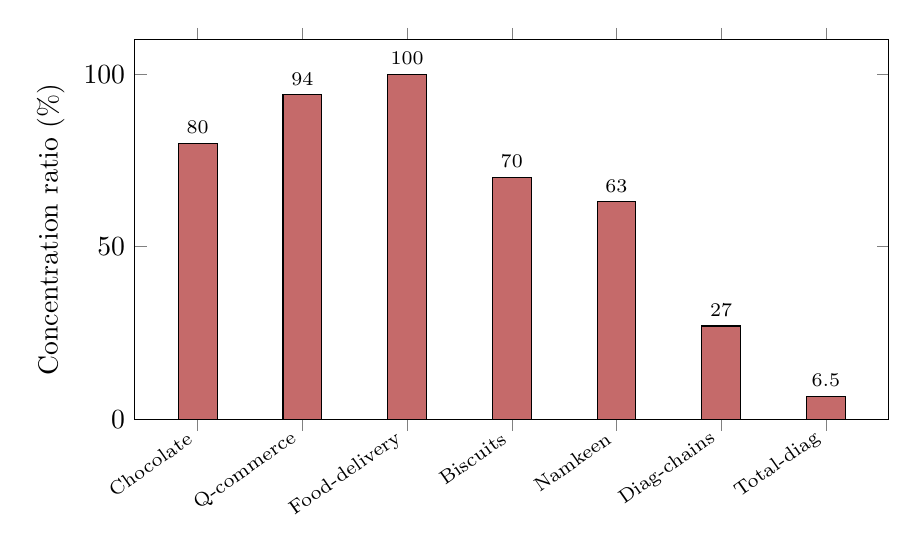
\begin{tikzpicture}
\begin{axis}[
  width=0.92\textwidth, height=6.4cm,
  ybar, bar width=14pt,
  ymin=0, ymax=110,
  ylabel={Concentration ratio (\%)},
  symbolic x coords={Chocolate,Q-commerce,Food-delivery,Biscuits,Namkeen,Diag-chains,Total-diag},
  xtick=data,
  x tick label style={rotate=35,anchor=east,font=\scriptsize},
  nodes near coords, nodes near coords style={font=\scriptsize},
  enlarge x limits=0.10,
]
\addplot[fill=uccol!65] coordinates {(Chocolate,80) (Q-commerce,94) (Food-delivery,100) (Biscuits,70) (Namkeen,63) (Diag-chains,27) (Total-diag,6.5)};
\end{axis}
\end{tikzpicture}
\caption{Market concentration across food \& platform segments (CR, \%): Chocolate CR4 80; Quick commerce CR3 94; Food delivery CR2 100; Biscuits CR3 70; Traditional namkeen CR4 63; Diagnostics-chains CR4 27 (mid 24--30); Total-diagnostics CR5 6.5. \textit{Source:} \cs{S189}; \cs{S190}; \cs{S193}; \cs{S164}; \cs{D:concentration\_food\_insurance\_tpa}.}
\label{fig:ch5food}
\end{figure}

\subsection{Quick Commerce and Food Delivery}

\VF\ (\emph{concentration}). Quick-commerce GMV is highly concentrated (Datum Intelligence, 2025): \textbf{Blinkit $\sim$48\%, Swiggy Instamart $\sim$24\%, Zepto $\sim$22\% $\rightarrow$ CR3 $\approx$ 94\%}; food delivery is a near-\textbf{duopoly} (Zomato/Eternal $\sim$55--58\% vs Swiggy $\sim$42--45\%, CR2 $\approx$ 100\% of the organized segment) \cs{S193}; \cs{D:quickcommerce\_delivery\_shares}. All three q-commerce leaders were built on \textbf{foreign} capital (Prosus/MIH, SoftBank, Tencent, Accel, Norwest; Zepto's foreign cap table incl. Nexus, Lightspeed, StepStone, Glade Brook, and \textbf{CalPERS} leading its 2025 round). Figure~\ref{fig:ch6qcomm} shows GMV shares.

% ---- FIGURE: CH6 quick-commerce GMV share ----
\begin{figure}[htbp]
\centering
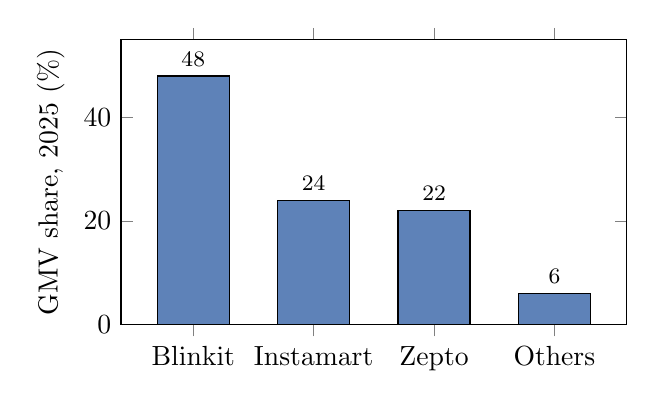
\begin{tikzpicture}
\begin{axis}[
  width=0.66\textwidth, height=5.2cm,
  ybar, bar width=26pt,
  ymin=0, ymax=55,
  ylabel={GMV share, 2025 (\%)},
  symbolic x coords={Blinkit,Instamart,Zepto,Others},
  xtick=data,
  nodes near coords, nodes near coords style={font=\footnotesize},
  enlarge x limits=0.2,
]
\addplot[fill=secol!70] coordinates {(Blinkit,48) (Instamart,24) (Zepto,22) (Others,6)};
\end{axis}
\end{tikzpicture}
\caption{Quick-commerce GMV share, 2025 (\%). \textit{Source:} Datum Intelligence, \cs{S193}; \cs{D:quickcommerce\_delivery\_shares}.}
\label{fig:ch6qcomm}
\end{figure}

\SE\ (\emph{the ``Indianization'' arc}). India's FDI/FEMA rule bars foreign capital from \emph{inventory-led} e-commerce (only \emph{marketplace} is 100\% automatic; inventory requires an \textbf{Indian-Owned-and-Controlled Company}, $>$50\% resident ownership; PN2/2018). Because q-commerce margins favour an inventory/private-label model, the leaders are restructuring: \textbf{Eternal capped foreign ownership at 49.5\%} (2025) and saw \textbf{Antfin/Alibaba fully exit} (Rs 5{,}370 cr, Aug 2025) \cs{S194}; \textbf{Zepto re-domiciled Singapore$\rightarrow$India} (NCLT, Jan 2025) \cs{S195}; \textbf{Swiggy's IOCC vote failed} (72.36\% vs 75\% needed, May 2026); \textbf{BigBasket} already became a Tata asset (foreign holders Alibaba/Actis exited, 2021) \cs{S196}. \textbf{Chinese-origin capital is being most aggressively unwound; US/European pension and institutional money is still flowing IN} (CalPERS$\rightarrow$Zepto) \cs{D:quickcommerce\_delivery\_shares}.

\subsection{Agriculture Inputs, Seeds and Cold Chain}

\VF\ --- but with a critical ownership/impact separation \cs{D:agritech\_inputs\_seeds}:
\begin{itemize}[leftmargin=1.4em,itemsep=2pt]
\item \textbf{Agritech aggregation} (DeHaat, Ninjacart, WayCool, Captain Fresh, Arya.ag, Samunnati, Stellapps) is mostly \textbf{minority foreign VC/growth/DFI/sovereign} capital (Temasek, Sofina, Prosus, Tiger, Walmart-Flipkart, Syngenta, IFC, FMO, Gates Foundation, Nuveen/TIAA), founders retaining control \cs{S197}. The \emph{documented} business model is \textbf{disintermediation} (cutting mandi middlemen), which companies argue \emph{raises} farmgate realization --- so the ``consolidation harms farmers'' thesis is, for these venture-stage platforms, a \PH, not a verified outcome.
\item \textbf{Seeds/inputs} is where concentration is empirically documented: \textbf{Mahyco Monsanto Biotech (now Bayer)} licensees command $\sim$90\% of the Bt-cotton trait market \cs{S199}; \textbf{KKR ($\sim$13.3\%, 2022) $+$ Alpha Wave ($\sim$12.5\%, 2024)} together hold $\sim$26\% of UPL's seeds platform \textbf{Advanta} \cs{S198}; FPIs hold $\sim$20\% of listed Kaveri Seed.
\item \textbf{Cold chain/warehousing} is the most FDI-open layer (100\% automatic): \textbf{Fairfax (Canada) controls $\sim$74\% of NCML} \cs{S200}, India's largest non-government grain handler --- the clearest control case in agri-logistics.
\end{itemize}

\SE\ Official baselines (NABARD NAFIS; MoSPI NSS-77) define the farmer context --- 93.1M agricultural households, $\sim$50.2\% indebted, crop-sale channels crop-specific --- and OECD evidence identifies the \emph{mechanisms} (input-side seed/trait power; downstream buyer/oligopsony power; trait-plus-chemistry bundling; data asymmetry) by which input/aggregation concentration \emph{could} compress farmer bargaining power \cs{S142}; \cs{S143}; \cs{S87}. \textbf{No source demonstrates that any named foreign-backed Indian platform has reduced farmer prices or bargaining power.} This is the central testable hypothesis, not a finding.

\subsection{Nutrition}\label{sec:nutrition}

Three layers, kept rigidly separate \cs{D:nutrition\_upf\_deep}.

\SE\ (\emph{nutrition science}). Converging meta-analytic evidence ties high UPF consumption to elevated chronic-disease risk: the \textbf{BMJ 2024 umbrella review} ($\sim$9.9M participants) graded CVD-mortality (RR 1.50), type-2-diabetes (RR 1.12/increment), anxiety and common mental disorders as ``convincing'' \cs{S201}; the \textbf{Lancet UPF Series (Nov 2025)} found 92 of 104 long-term studies showed elevated risk across 12 conditions \cs{S202}. (Observational-dominated; NOVA classification contested --- so directionally robust, not RCT-grade proof.)

\VF\ (\emph{India burden and market}). India carries a vast metabolic-NCD burden (\textbf{ICMR-INDIAB: 101M diabetic, 254M generally obese, 2021}) and is among the fastest-growing UPF markets (\textbf{Economic Survey 2024-25: UPF retail sales $\sim$US\$0.9bn in 2006 $\rightarrow$ $\sim$US\$38bn in 2019}) \cs{S203}. WHO India reports UPF retail value grew 13.37\% CAGR (2011--21), salty snacks 16.78\% \cs{S54}; ICMR-NIN attributes 56.4\% of India's disease burden to unhealthy diets \cs{S53}. A 2024 lab study found all 23 tested packaged chips exceeded $\ge$1 HFSS threshold, with significant label-vs-lab discrepancies \cs{S204}. India's FSSAI front-of-pack ``Indian Nutrition Rating'' warning-label regime remains \textbf{stalled} amid industry resistance. Figures~\ref{fig:ch7upf} and \ref{fig:ch8metabolic} quantify the market and burden.

\PH\ / \UC\ (\emph{PE causation}). Whether foreign capital \emph{causes} worse nutrition outcomes --- via reformulation, portion inflation, marketing-to-children, or deeper rural distribution --- is \textbf{not established} for the specific Indian deals. What is documented: foreign capital has scaled the HFSS categories, capital is raised explicitly ``for expansion/distribution,'' and global UPF-industry playbooks (marketing, lobbying against warning labels) are well documented. The synthesis: \textbf{correlation and capacity-building, not a proven causal chain} from any individual deal to population harm.

% ---- FIGURE: CH7 UPF retail sales 2006 vs 2019 ----
\begin{figure}[htbp]
\centering
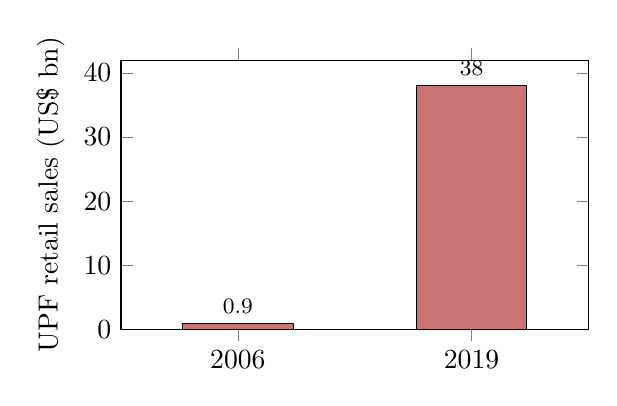
\begin{tikzpicture}
\begin{axis}[
  width=0.62\textwidth, height=5.0cm,
  ybar, bar width=40pt,
  ymin=0, ymax=42,
  ylabel={UPF retail sales (US\$ bn)},
  symbolic x coords={2006,2019},
  xtick=data,
  nodes near coords, nodes near coords style={font=\footnotesize},
  enlarge x limits=0.5,
]
\addplot[fill=uccol!60] coordinates {(2006,0.9) (2019,38)};
\end{axis}
\end{tikzpicture}
\caption{India ultra-processed-food retail sales (US\$ bn): 2006 $\sim$0.9; 2019 $\sim$38. Implies $\sim$13.4\% CAGR (WHO 2011--21). \textit{Source:} Economic Survey 2024-25, \cs{S203}; WHO India \cs{S54}.}
\label{fig:ch7upf}
\end{figure}

% ---- FIGURE: CH8 metabolic burden ----
\begin{figure}[htbp]
\centering
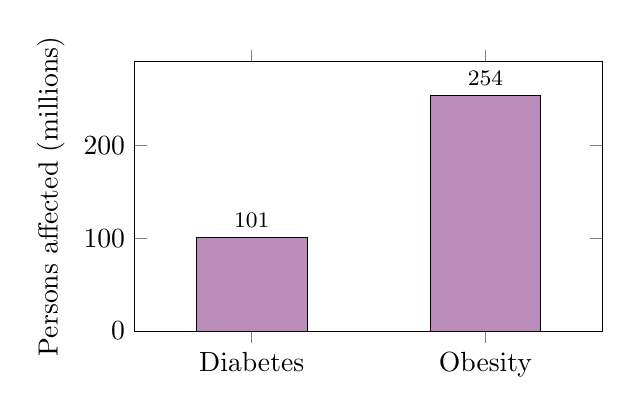
\begin{tikzpicture}
\begin{axis}[
  width=0.62\textwidth, height=5.0cm,
  ybar, bar width=40pt,
  ymin=0, ymax=290,
  ylabel={Persons affected (millions)},
  symbolic x coords={Diabetes,Obesity},
  xtick=data,
  nodes near coords, nodes near coords style={font=\footnotesize},
  enlarge x limits=0.5,
]
\addplot[fill=phcol!60] coordinates {(Diabetes,101) (Obesity,254)};
\end{axis}
\end{tikzpicture}
\caption{India metabolic-disease burden, 2021 (millions, ICMR-INDIAB): Diabetes 101; generalised obesity 254. \textit{Source:} ICMR-INDIAB, \cs{S203}.}
\label{fig:ch8metabolic}
\end{figure}

% =====================================================================
\section{Concentration Analysis --- The Central Paradox}\label{sec:concentration}
% =====================================================================
This section consolidates the new computed concentration evidence. \textbf{The central paradox:} national concentration is \emph{low} (so ``monopolized'' is unsupported), but the small \emph{organized} tier --- where foreign PE/sovereign capital is concentrated --- is consolidating fast, and \emph{local} (city/specialty) concentration is real but unmeasured. State the denominator with every ratio.

\subsection{Hospitals --- bed-ownership census and CR/HHI}

The 14-largest-chain organized bed census ($\sim$69{,}700 beds, mixed capacity/operational basis) is given in Table~\ref{tab:bedcensus} \cs{D:hospital\_bed\_ownership\_map}.

\begin{table}[htbp]
\centering
\small
\caption{The 14-chain organized bed-ownership class shares ($\sim$69{,}700 beds). \textit{Source:} \cs{D:hospital\_bed\_ownership\_map}.}
\label{tab:bedcensus}
\begin{tabularx}{\textwidth}{@{}>{\raggedright\arraybackslash}X r r@{}}
\toprule
\textbf{Ownership class} & \textbf{Beds} & \textbf{Share of organized sample} \\
\midrule
Foreign-PE controlled (Blackstone/QCIL, KKR/HCG) & $\sim$13{,}125 & 18.8\% \\
Foreign-sovereign controlled (Temasek/Manipal) & $\sim$12{,}367 & 17.7\% \\
\textbf{Foreign PE $+$ sovereign} & \textbf{$\sim$25{,}492} & \textbf{36.6\%} \\
Foreign-strategic (IHH: Fortis $+$ Gleneagles) & $\sim$6{,}250 & 9.0\% \\
\textbf{All foreign-controlled} & \textbf{$\sim$31{,}742} & \textbf{45.6\%} \\
Domestic / listed-dispersed / family & $\sim$37{,}934 & 54.4\% \\
\midrule
\textbf{CR4} (Manipal, Aster-QCIL, Apollo, Narayana) & $\sim$39{,}134 & \textbf{56.2\%} \\
\textbf{CR8} ($+$ KIMS, Max, Fortis, Medanta) & $\sim$57{,}598 & \textbf{82.7\%} \\
\bottomrule
\end{tabularx}
\end{table}

\textbf{Resolution of repository claim ``$\sim$25\% of organized beds PE-controlled'' --- partially verified / denominator-dependent} (Table~\ref{tab:denominator}). \EI

\begin{table}[htbp]
\centering
\small
\caption{The ``25\% claim'' is denominator-dependent. \textit{Source:} \cs{D:hospital\_bed\_ownership\_map}; \cs{D:concentration\_hospitals\_diagnostics}.}
\label{tab:denominator}
\begin{tabularx}{\textwidth}{@{}>{\raggedright\arraybackslash}X r r@{}}
\toprule
\textbf{Denominator} & \textbf{Foreign-PE$+$sovereign share} & \textbf{All-foreign-controlled share} \\
\midrule
ICRA organized large-chain pool ($\sim$56{,}000--71{,}000 beds) & \textbf{$\sim$36--46\%} & \textbf{$\sim$45--57\%} \\
Implied all-private beds ($\sim$1.122M) & $\sim$2.3\% & $\sim$2.8\% \\
All-India total beds proxy ($\sim$1.886M) & $\sim$1.35\% & $\sim$1.7\% \\
\bottomrule
\end{tabularx}
\end{table}

\SE\ On the organized-large-chain denominator the ``25\% PE-controlled'' figure is \emph{conservative}; on any all-India/all-private denominator it collapses to 1--3\%. Crucially, \textbf{sovereign (Temasek) and strategic (IHH) control is at least as large as classic-PE control} and is routinely mis-labelled ``PE.'' Per CRISIL/KPMG, the corporate hospital tier is itself only $\sim$25--35\% of \emph{private} delivery; the top-4 corporate chains' \textbf{national CR4 $\approx$ 16--24\% of the organized pool} and national \textbf{HHI is well under 1{,}000} \cs{D:concentration\_hospitals\_diagnostics}. \textbf{National monopolization is unsupported.} The denominator-dependence is visualized in Figure~\ref{fig:ch2denom}; the organized-pool concentration in Figure~\ref{fig:ch3conc}.

\EI\ (\emph{where the real risk sits}). Hospital markets are \emph{local}. No public source publishes city-level CR4/HHI, but the qualitative signals are clear: oncology (KKR/HCG $\sim$2{,}500 beds), maternity/fertility (AHH/GIC, Cloudnine, Rainbow), and specific metros (Hyderabad --- KIMS $+$ CARE/Blackstone; parts of NCR; Bengaluru) plausibly show single-platform shares far above national levels. \textbf{Local and specialty concentration --- not national CR4 --- is the legitimate, currently-unmeasured concern.} KPMG: ``most parts of the country (except North-East) are today covered by a PE-fund-backed multi-specialty platform.''

% ---- FIGURE: CH2 denominator-dependent ----
\begin{figure}[htbp]
\centering
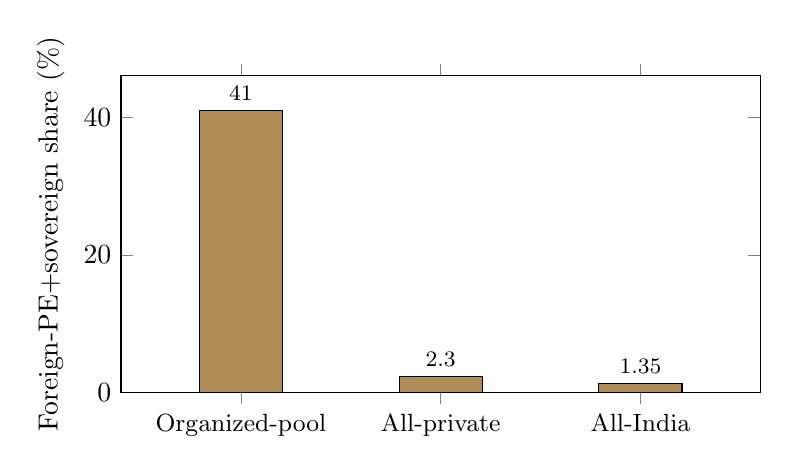
\begin{tikzpicture}
\begin{axis}[
  width=0.80\textwidth, height=5.6cm,
  ybar, bar width=30pt,
  ymin=0, ymax=46,
  ylabel={Foreign-PE$+$sovereign share (\%)},
  symbolic x coords={Organized-pool,All-private,All-India},
  xtick=data,
  x tick label style={font=\small},
  nodes near coords, nodes near coords style={font=\footnotesize},
  enlarge x limits=0.3,
]
\addplot[fill=eicol!70] coordinates {(Organized-pool,41) (All-private,2.3) (All-India,1.35)};
\end{axis}
\end{tikzpicture}
\caption{The ``$\sim$25\% of organized beds'' claim is denominator-dependent (foreign-PE$+$sovereign share, \%): ICRA organized large-chain pool 41 (range 36--46); implied all-private beds 2.3; all-India total beds 1.35. \textit{Source:} \cs{D:hospital\_bed\_ownership\_map}.}
\label{fig:ch2denom}
\end{figure}

% ---- FIGURE: CH3 organized concentration ----
\begin{figure}[htbp]
\centering
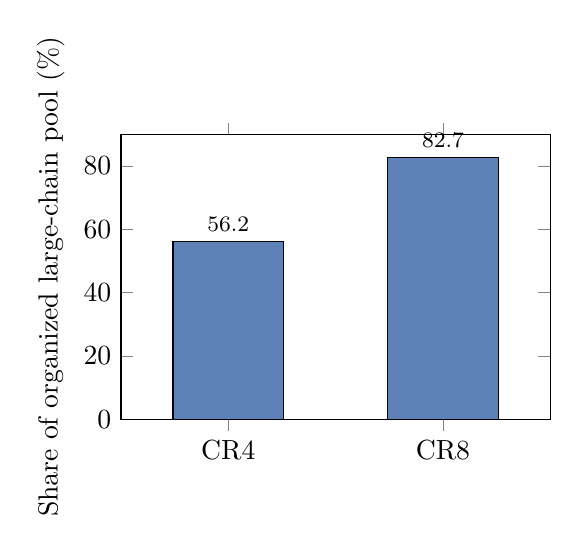
\begin{tikzpicture}
\begin{axis}[
  width=0.58\textwidth, height=5.2cm,
  ybar, bar width=40pt,
  ymin=0, ymax=90,
  ylabel={Share of organized large-chain pool (\%)},
  symbolic x coords={CR4,CR8},
  xtick=data,
  nodes near coords, nodes near coords style={font=\footnotesize},
  enlarge x limits=0.5,
]
\addplot[fill=secol!70] coordinates {(CR4,56.2) (CR8,82.7)};
\end{axis}
\end{tikzpicture}
\caption{Organized-hospital concentration (share of organized large-chain bed pool, \%): CR4 56.2; CR8 82.7. National CR4 of the corporate pool is only $\sim$16--24\% (HHI $<$1{,}000). \textit{Source:} \cs{D:hospital\_bed\_ownership\_map}; \cs{D:concentration\_hospitals\_diagnostics}.}
\label{fig:ch3conc}
\end{figure}

\subsection{Diagnostics, food, insurance, TPA --- consolidated CR/HHI}

The consolidated cross-market concentration picture is given in Table~\ref{tab:crhhi}.

\begin{table}[htbp]
\centering
\small
\setlength{\tabcolsep}{4pt}
\caption{Consolidated CR/HHI across markets. \textit{Source:} \cs{D:concentration\_hospitals\_diagnostics}; \cs{D:concentration\_food\_insurance\_tpa}; \cs{D:quickcommerce\_delivery\_shares}.}
\label{tab:crhhi}
\begin{tabularx}{\textwidth}{@{}>{\raggedright\arraybackslash}p{4.0cm} >{\raggedright\arraybackslash}p{4.3cm} >{\raggedright\arraybackslash}p{3.2cm} >{\raggedright\arraybackslash}X@{}}
\toprule
\textbf{Market} & \textbf{Best metric} & \textbf{Verdict} & \textbf{Foreign-capital intensity} \\
\midrule
Diagnostics (total) & CR5 $\sim$6--7\%; leader $<$6\% in home region & Fragmented (consolidating) & Backers of consolidators foreign \\
Diagnostics (organized chains slice, $\sim$20--24\% of total) & CR4 $\sim$24--30\% & Moderate within a minority slice & High \\
Traditional/ethnic namkeen & Haldiram $\sim$38.5\%; CR4 $\sim$63\% & Moderately concentrated & Rising (Temasek/IHC/AW minority) \\
Total savoury snacks (broad) & Haldiram $\sim$13\%; large unorganized tail & Low & Mixed \\
Biscuits & CR3 $\sim$70\%$+$ (Britannia/Parle/ITC) & Concentrated & Low (mostly Indian) \\
Chocolate & CR1 $\sim$55--65\% (Mondelez); CR4 $\sim$80\% & Highly concentrated & Very high --- foreign strategic MNCs \\
Overall health insurance & HHI $\sim$700--830; CR4 $\sim$43.5\% & NOT concentrated & Moderate (foreign at insurer level) \\
Retail health insurance & CR3 $\sim$52\% (Star$+$Care$+$Niva); SAHIs $\sim$56\% & Moderately concentrated & High (Bupa/Cigna/ADIA JVs) \\
TPA (claims layer) & CR4 $\sim$68\%; Medi Assist $\sim$31\%$\rightarrow$37\% & Concentrated \& consolidating & High (Bessemer/Investcorp-built leader) \\
Quick commerce (GMV) & CR3 $\sim$94\% (Blinkit/Instamart/Zepto) & Highly concentrated & Foreign-built; Indianizing \\
Food delivery (GMV) & CR2 $\sim$100\% (Zomato/Swiggy) & Duopoly & Foreign-built; Indianizing \\
\bottomrule
\end{tabularx}
\end{table}

\SE\ Concentration and foreign-capital intensity \textbf{rise as one moves down the value chain and into the most data-/margin-rich sub-segments} --- from fragmented overall insurance, to a more-concentrated retail-health/SAHI tier with foreign JV partners, to a highly concentrated TPA claims layer built by foreign PE; and from a broad, fragmented savoury-snacks universe to a concentrated \emph{chocolate} category held by foreign strategic MNCs. The platform-economy segments (q-commerce CR3 $\sim$94\%, food-delivery duopoly) are the most concentrated of all and the most foreign-built --- but are being forced toward Indian control by FDI rules \cs{D:concentration\_food\_insurance\_tpa}; \cs{D:quickcommerce\_delivery\_shares}. Figure~\ref{fig:ch4chain} shows the rising-concentration gradient down the health-financing chain.

% ---- FIGURE: CH4 concentration rises down chain (CR) ----
\begin{figure}[htbp]
\centering
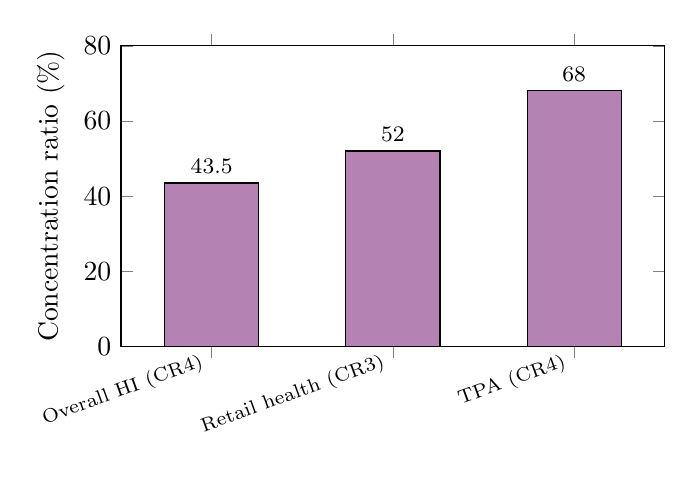
\begin{tikzpicture}
\begin{axis}[
  width=0.70\textwidth, height=5.4cm,
  ybar, bar width=34pt,
  ymin=0, ymax=80,
  ylabel={Concentration ratio (\%)},
  symbolic x coords={OverallHI,RetailHealth,TPA},
  xtick=data,
  xticklabels={Overall HI (CR4),Retail health (CR3),TPA (CR4)},
  x tick label style={rotate=20,anchor=east,font=\scriptsize},
  nodes near coords, nodes near coords style={font=\footnotesize},
  enlarge x limits=0.25,
]
\addplot[fill=phcol!65] coordinates {(OverallHI,43.5) (RetailHealth,52) (TPA,68)};
\end{axis}
\end{tikzpicture}
\caption{Concentration rises down the health value chain (CR, \%): Overall health insurance CR4 43.5; Retail health CR3 52; TPA CR4 68. (Overall health-insurance HHI $\sim$765, midpoint of 700--830, sits above the moderately-concentrated floor of $\sim$1{,}500 only at the retail/TPA tiers.) \textit{Source:} \cs{D:concentration\_food\_insurance\_tpa}; \cs{S79}; \cs{S186}; \cs{S187}.}
\label{fig:ch4chain}
\end{figure}

% =====================================================================
\section{Value-Extraction Mechanisms --- Global Playbook vs Documented India Status}\label{sec:valueextraction}
% =====================================================================
The US/Europe evidence (\S\ref{sec:international}) documents a six-part value-extraction playbook. The decisive India finding is that \textbf{the most aggressive financial-engineering tools are largely latent in India; the operative lever is ARPOB escalation, which is not PE-specific} \cs{D:value\_extraction\_india\_hospitals}. The scorecard is given in Table~\ref{tab:valuescorecard}.

\begin{table}[htbp]
\centering
\small
\setlength{\tabcolsep}{4pt}
\caption{Value-extraction scorecard: global playbook vs documented India status. \textit{Source:} \cs{D:value\_extraction\_india\_hospitals}; \cs{S205}; \cs{S209}; \cs{S210}.}
\label{tab:valuescorecard}
\begin{tabularx}{\textwidth}{@{}>{\raggedright\arraybackslash}p{3.2cm} >{\raggedright\arraybackslash}p{3.3cm} >{\raggedright\arraybackslash}p{3.4cm} >{\raggedright\arraybackslash}X@{}}
\toprule
\textbf{Mechanism} & \textbf{Global evidence} & \textbf{India status} & \textbf{Best India evidence} \\
\midrule
Dividend recapitalization & Strong (NBER WP 33435) & Hypothesized --- not documented at scale & None found; constrained by SEBI/Companies Act \\
Sale-leaseback / hospital REIT & Strong (Harvard: REIT hospitals $>$5x closure risk; Steward/MPT) & Partial / mostly absent --- no listed healthcare REIT & Fortis$\rightarrow$Religare Health Trust (Singapore, 2012), \emph{unwound} 2019 (Rs 4{,}650 cr buyback) \\
Management/monitoring fees & Definitional & Hypothesized --- no figures found & Fortis--RHT service/lease fees \\
Debt loading / leverage & Strong (NBER) & Partial / deal-level only; listed balance sheets conservative & \textbf{HCG gearing 2.08x$\rightarrow$3.59x post-KKR (FY25)} --- clearest signal; Max net-cash$\rightarrow$net-debt (D/E $\sim$0.32) \\
Buy-and-build roll-up & Strong & Documented \& prominent & Blackstone/QCIL$\rightarrow$Aster; Manipal; KKR/HCG; AHH/GIC \\
ARPOB / price escalation & Strong (US ED markups) & Documented --- THE India lever & ICRA: industry ARPOB $+$11\% FY24, $+$7\% FY25; all listed chains; OPM $\sim$23.6\% \\
Clinical-quality harm & Strong (JAMA $+$25.4\%) & Hypothesized for India --- unverified & No India PE-vs-non-PE quality study exists \\
\bottomrule
\end{tabularx}
\end{table}

\EI\ Indian listed hospitals (Apollo ARPOB $\sim$Rs 60{,}588/day; Max $\sim$Rs 77{,}000; Medanta $\sim$Rs 62{,}000; HCG $\sim$Rs 44{,}041) earn high-20s/low-30s EBITDA margins on rising ARPOB, occupancy 60--77\%, and a payer mix shifting to cash$+$insurance --- \emph{even where PE has fully exited} (Max, post-KKR, has the sector's highest ARPOB under founder control). This shows the \textbf{listed-chain economics, not financial engineering, are the India value story}: rising ARPOB feeds $\sim$14\% medical inflation and the AHPI-vs-insurer tariff disputes (AHPI's 2025 cashless-suspension threat against Bajaj Allianz/Care). The \textbf{Singh-brothers/Religare fraud} at Fortis (Rs 2{,}473 cr diverted; SEBI/SFIO actions) is extreme \emph{related-party} extraction --- fraud, not the standard PE playbook --- and \emph{pre-dates} IHH's foreign control \cs{D:value\_extraction\_india\_hospitals}. ARPOB by listed chain is shown in Figure~\ref{fig:ch12arpob}.

% ---- FIGURE: CH12 ARPOB ----
\begin{figure}[htbp]
\centering
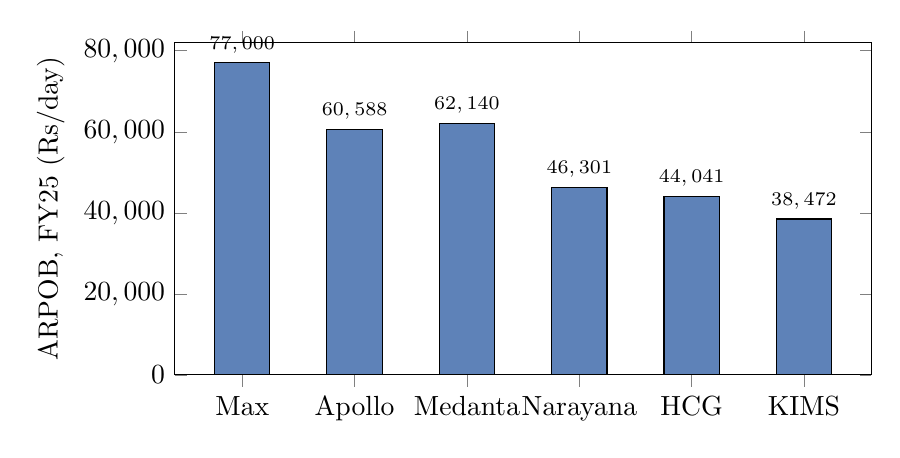
\begin{tikzpicture}
\begin{axis}[
  width=0.86\textwidth, height=5.8cm,
  ybar, bar width=20pt,
  ymin=0, ymax=82000,
  ylabel={ARPOB, FY25 (Rs/day)},
  symbolic x coords={Max,Apollo,Medanta,Narayana,HCG,KIMS},
  xtick=data,
  scaled y ticks=false,
  yticklabel style={/pgf/number format/fixed,/pgf/number format/1000 sep={,}},
  nodes near coords, nodes near coords style={font=\scriptsize,/pgf/number format/1000 sep={,}},
  enlarge x limits=0.12,
]
\addplot[fill=secol!70] coordinates {(Max,77000) (Apollo,60588) (Medanta,62140) (Narayana,46301) (HCG,44041) (KIMS,38472)};
\end{axis}
\end{tikzpicture}
\caption{Indian listed-hospital ARPOB, FY25 (Rs/day). Industry ARPOB rose $\sim$7\% in FY25 (ICRA), feeding $\sim$14\% medical inflation; Max's sector-high ARPOB is under founder control post-KKR exit. \textit{Source:} company FY25 presentations \cs{S166}; ICRA \cs{S209}.}
\label{fig:ch12arpob}
\end{figure}

% =====================================================================
\section{Policy and Regulatory Architecture}\label{sec:policy}
% =====================================================================
\subsection{FDI policy --- sector-precise chronology}

\VF\ \cs{D:fdi\_price\_control\_timeline}. The net direction across every relevant sector has been \emph{toward more foreign ownership with less prior scrutiny}, with two counter-moves (brownfield pharma 2011; the 2020 China land-border restriction). Table~\ref{tab:fdiroute} gives the sector-by-sector position.

\begin{table}[htbp]
\centering
\small
\caption{FDI route and chronology by sector. \textit{Source:} \cs{S227}; \cs{D:fdi\_price\_control\_timeline}.}
\label{tab:fdiroute}
\begin{tabularx}{\textwidth}{@{}>{\raggedright\arraybackslash}p{3.6cm} >{\raggedright\arraybackslash}p{4.6cm} >{\raggedright\arraybackslash}X@{}}
\toprule
\textbf{Sector} & \textbf{FDI position} & \textbf{Key instrument/date} \\
\midrule
Hospitals \& diagnostics & 100\% automatic since $\sim$Jan 2000 & (never a binding constraint) \\
Pharma greenfield & 100\% automatic throughout & --- \\
Pharma brownfield & $\rightarrow$approval route (2011) $\rightarrow$ 74\% automatic / $>$74\% approval (2016) & PN3/2011; PN5/2016 (24 Jun 2016); conditions: maintain NLEM output, R\&D, no non-compete \\
Medical devices & 100\% automatic (carve-out) & Cabinet 26 Dec 2014; PN2/2015 \\
Multi-brand retail & 51\% Government route (largely dead letter) & PN5/2012 (20 Sep 2012) \\
Food-product retail (incl. e-commerce of India-made food) & 100\% (Government route per DPIIT) & Budget 2016; operationalized 20 Jun 2016 \\
E-commerce & marketplace 100\% automatic; inventory-led prohibited (IOCC required) & PN2/2018 (eff. 1 Feb 2019) \\
Insurance & 26\%$\rightarrow$49\% (2015)$\rightarrow$74\% (2021)$\rightarrow$100\% (in force 5 Feb 2026) & Sabka Bima Sabki Raksha Act 2025 \\
\bottomrule
\end{tabularx}
\end{table}

\textbf{Correction carried from baseline:} the repository's claim that ``food \& beverage'' was newly opened to 100\% FDI in January 2025 is wrong; food-product retail trading was opened in 2016 (Government route), and it is \emph{insurance} that moved to 100\% in 2025.

\subsection{Price control --- DPCO/NPPA}

\VF\ DPCO 2013 (15 May 2013) set market-based ceilings for NLEM drugs; NPPA capped \textbf{coronary stents ($\sim$85\% cut, Feb 2017)} and \textbf{knee implants (Aug 2017)} under Para 19 powers, and launched \textbf{trade-margin rationalization} (42 anti-cancer drugs, $\sim$30\% margin cap, 2019; COVID devices, 70\%, 2021). Hospital \emph{services} are not nationally price-capped. The stent-cap experience produced a \textbf{documented unintended consequence} (hospitals raised consumables/procedure/doctor charges to recoup margin), and a 2019 parliamentary answer noted reviewed stent-overcharging complaints usually found no direct stent overcharging --- so the repository's ``systemwide procedure-fee shifting'' claim should be narrowed to a billing-transparency/non-stent-component monitoring risk \cs{S121}--\cs{S124}; \cs{S228}; \cs{D:india\_impact\_evidence\_hunt}.

\subsection{Tax, treaty routing and GIFT-City structuring (new)}\label{sec:tax}

\VF\ \cs{D:tax\_treaty\_structuring}. The structuring architecture that enables foreign capital at near-zero exit tax:
\begin{itemize}[leftmargin=1.4em,itemsep=2pt]
\item \textbf{Pre-2017:} India--Mauritius and India--Singapore treaties taxed Indian-share capital gains only in the (zero-rate) residence state $\rightarrow$ effective zero exit tax; $\sim$34\% of cumulative FDI (2000--17) routed via Mauritius, $\sim$16\% via Singapore.
\item \textbf{2016 protocols $\rightarrow$ source-based taxation from 1 Apr 2017,} with \textbf{grandfathering} for pre-April-2017 shares; \textbf{GAAR effective 1 Apr 2017; MLI/PPT from FY2020-21}. Routing shifted \textbf{Mauritius $\rightarrow$ Singapore} (Singapore overtook Mauritius as top FDI source by FY2018-19) and toward \textbf{GIFT-City IFSC} \cs{S211}.
\item \textbf{GIFT-City IFSC:} \S80LA 10-year tax holiday; \S10(4D)/\S115AD concessions for Category-III IFSC AIFs; \textbf{tax-neutral relocation of offshore funds} (\S47(viiac)/(viiad), sunset extended to 2030). IFSCA reports 194 FMEs / $>$US\$32bn commitments by Q3 FY26 \cs{S114}--\cs{S116}.
\item \textbf{Finance (No.2) Act 2024:} LTCG \textbf{12.5\%}, STCG 20\%, \textbf{indexation removed} (NRIs excluded from resident relief), \textbf{buyback-as-deemed-dividend} from 1 Oct 2024 \cs{S212}.
\item \textbf{Transparency lever:} SEBI's 2023--24 \textbf{FPI beneficial-ownership look-through} (full natural-person disclosure for high-risk FPIs) is the primary public tool to pierce offshore structures \cs{S213}.
\end{itemize}

\EI\ The architecture is \emph{legal}; the public-interest concerns are (a) erosion of India's tax base on the appreciation of strategic Indian assets, (b) opacity of ultimate beneficial ownership (visible mainly in CCI orders and SEBI BO filings), and (c) round-tripping risk flagged by the Government's own 2012 Black Money White Paper. No specific transaction is shown to involve unlawful evasion.

\subsection{Health financing and PM-JAY}

\VF\ Latest official NHA 2022-23: government health expenditure \textbf{1.43\% of GDP} (1.48\% new series); out-of-pocket \textbf{43.4\% of THE} \cs{S08} --- below the NHP 2017 target of 2.5\% by 2025, but the repository's ``current 54.8\% OOPE'' is outdated. NSS 2017-18 hospitalization expenditure (ex-childbirth) was \textbf{$\sim$7.15x higher in private than public} facilities \cs{S127} --- large, but not proven PE-caused. \textbf{AB-PMJAY} covers 12 crore families with \textbf{$>$15{,}733 private hospitals empanelled} by Dec 2025 \cs{S74}; \cs{S75}; peer-reviewed evidence shows \emph{uneven} participation (e.g., only 13\% of private hospitals in Maharashtra; few large/premium chains) and significant fraud/de-empanelment (\S\ref{sec:indiaimpact}) \cs{S137}; \cs{S138}. NITI Aayog/Brookings: $>$7\% of the population is pushed into poverty yearly by health costs \cs{S125}. Latest financing indicators are consolidated in Table~\ref{tab:financing}.

\begin{table}[htbp]
\centering
\small
\caption{Latest official health-financing indicators. \textit{Source:} as cited.}
\label{tab:financing}
\begin{tabularx}{\textwidth}{@{}>{\raggedright\arraybackslash}X r >{\raggedright\arraybackslash}p{2.0cm} l@{}}
\toprule
\textbf{Indicator} & \textbf{Value} & \textbf{Source} & \textbf{Class.} \\
\midrule
Government health expenditure (\% of GDP), 2022-23 & 1.43\% (old) / 1.48\% (new series) & \cs{S08} & VF \\
Government health expenditure (\% of THE), 2022-23 & 43.7\% & \cs{S08} & VF \\
Out-of-pocket expenditure (\% of THE), 2022-23 & 43.4\% & \cs{S08} & VF \\
NHP public-health-spend target (\% of GDP by 2025) & 2.5\% (not met) & \cs{S06}--\cs{S08} & VF \\
Population pushed into poverty yearly by health costs & $>$7\% & \cs{S125} & SE \\
Private/public hospitalization expenditure ratio (NSS 2017-18, ex-childbirth) & $\sim$7.15x & \cs{S127} & VF \\
AB-PMJAY private hospitals empanelled (Dec 2025) & $>$15{,}733 & \cs{S74}; \cs{S75} & VF \\
Health-insurance gross premium (FY25, ex-PA/travel) & Rs 1{,}17{,}504.82 cr & \cs{S79} & VF \\
Health claims settled / paid (FY25) & 3.26 cr / Rs 94{,}248 cr & \cs{S79} & VF \\
Share of settled claim counts via TPAs (FY25) & 69\% & \cs{S79} & VF \\
\bottomrule
\end{tabularx}
\end{table}

% =====================================================================
\section{Influence, Lobbying and Governance (Documented Channels)}\label{sec:influence}
% =====================================================================
\textbf{Scope caveat (\VF).} India has \textbf{no statutory lobbying-disclosure regime}, so most influence activity is structurally invisible; this section documents \emph{provable channels and interlocks} and marks capture/quid-pro-quo as \UC\ unless specifically documented \cs{D:lobbying\_associations\_governance}.

\VF\ --- the channels:
\begin{itemize}[leftmargin=1.4em,itemsep=2pt]
\item \textbf{The PE/VC apex lobby (IVCA)} --- 490$+$ members, $>$US\$350bn AUM, openly ``advocating regulatory interventions'' --- has its Executive Committee \textbf{officered by the India heads of Blackstone, KKR, Warburg Pincus, Bain Capital, and CPP Investments}, with ChrysCapital and Everstone on its leadership, and \textbf{ex-Commerce-Secretary Anup Wadhawan} (also a GSK India board member, ex-IRDAI part-time member) on its board --- the cleanest revolving-door interlock spanning trade, insurance regulation, PE and pharma. IVCA's verified policy wins include the Budget-2025 AIF/IFSC tax clarifications \cs{S214}.
\item \textbf{Provider associations led by PE-backed operators:} \textbf{NATHEALTH} President is Max Healthcare's Abhay Soi (ex-KKR control); officers run Metropolis, Apollo, Dr Lal, Healthium; \textbf{FICCI Health Services} is co-chaired by Quality Care/Blackstone-TPG's Varun Khanna; \textbf{CII Pharma} chaired by Dr Reddy's. AHPI's 2025 cashless-suspension bloc against Bajaj Allianz shows associations as \emph{operational} power centres \cs{S215}.
\item \textbf{Foreign device lobby $\rightarrow$ trade pressure:} \textbf{AdvaMed's USTR petition} over India's stent/knee price caps contributed to the \textbf{US withdrawal of India's GSP benefits (5 Jun 2019, $\sim$3{,}600 product lines)} --- a documented cross-border lobbying chain \cs{S216}.
\item \textbf{Industry seated in its own regulator:} the Department of Pharmaceuticals' March 2024 drug-pricing-reform committee included \textbf{IPA and IDMA as ``special invitees''} --- which public-health groups (AIDAN) characterized as ``capture'' (the characterization is an allegation; the composition is fact) \cs{S217}.
\item \textbf{US councils (USISPF/USIBC)} publicly lobbied for the \textbf{100\% insurance FDI} (passed Dec 2025) and against data localization.
\item \textbf{Political finance:} pharma/healthcare firms bought \textbf{$\sim$Rs 800--903 cr of electoral bonds (2019--24)} (Dr Reddy's Rs 80 cr top), with a \emph{documented correlation} between several donors and contemporaneous drug-quality failures --- \textbf{quid-pro-quo unproven}; foreign PE does not directly buy bonds (link is indirect/attenuated) \cs{S218}.
\item A \textbf{2012 Parliamentary Standing Committee} found a ``collusive nexus'' between drug manufacturers and CDSCO --- the strongest \emph{official} statement of capture risk.
\end{itemize}

\SE\ Foreign institutional capital's policy interface is \emph{embedded in the association-leadership layer} (alignment-by-design), not exercised as overt, disclosed lobbying. \textbf{Regulatory capture is not established}, but the density of interlocks, the seating of regulated industry inside rule-drafting bodies, the GSP episode, and the donation/drug-quality correlation collectively justify a transparency-and-conflict-of-interest inquiry.

% =====================================================================
\section{India-Specific Impact Evidence (Price, Quality, Access)}\label{sec:indiaimpact}
% =====================================================================
\textbf{Critical caveat (the central limit on causation).} Documented harms below are \textbf{corporate/private-sector-wide}; \textbf{no located India study isolates PE-owned vs domestically-owned private-hospital outcomes} with a clean counterfactual, and the strongest academic source (Hunter et al. 2025, \emph{Sociology of Health \& Illness}) is \emph{qualitative}. Several flagship incidents \emph{pre-date} the foreign-control events at those chains \cs{S223}; \cs{D:india\_impact\_evidence\_hunt}.

\VF\ (\emph{the documented record}):
\begin{itemize}[leftmargin=1.4em,itemsep=2pt]
\item \textbf{Regulator (NPPA) mark-ups:} at four NCR private hospitals, billed-vs-purchase mark-ups of \textbf{1{,}737\% (three-way stop cock), 1{,}271\% (IV set), 1{,}208\% (syringe), 1{,}192\% (non-scheduled drug), 357\% (scheduled drug)}; drugs/devices/diagnostics $=$ 56\% of bills \cs{S31}; \cs{S219}. The NPPA chairman was transferred $\sim$8 days later (retaliation \UC) \cs{S128}; \cs{S129}.
\item \textbf{Supplier-induced demand (peer-reviewed):} private-vs-public C-section odds ratio rose \textbf{1.62 (2005-06) $\rightarrow$ 4.17 (2015-16)}; NFHS-5: \textbf{47.4\% private vs 14.3\% public}; $\sim$1.83M avoidable C-sections/yr; insurance-driven unnecessary hysterectomies ($\sim$16{,}000 in Bihar 2011; $\sim$70\% in private). PLOS Medicine systematic review: LMIC private providers more often violated standards \cs{S220}.
\item \textbf{COVID-era overcharging (Maharashtra audits):} 82.5\% of audited episodes overcharged; critical-care bills 400--500\% above caps; BMC forced $\sim$Rs 14 cr refunds on $\sim$Rs 112 cr screened --- \emph{large hospitals overcharged at higher frequency} (a size, not ownership, effect) \cs{S221}.
\item \textbf{AB-PMJAY fraud:} \textbf{1{,}114 hospitals de-empanelled, 549 suspended, 1{,}504 penalised Rs 122 cr; 342{,}988 fraud cases incl. $>$56{,}000 fraudulent/unnecessary surgeries}; the Khyati Hospital (Ahmedabad) angioplasty-deaths case (Nov 2024, 2 deaths, 8 arrested). NHA data are \emph{not} ownership-disaggregated \cs{S222}.
\item \textbf{Ethics/negligence incidents:} Fortis Adya Singh dengue (2017, $\sim$Rs 16 lakh bill, govt found ``grave negligence'') --- \emph{before} IHH control (Nov 2018); Max Shalimar Bagh newborn-wrongly-declared-dead (2017, licence cancelled then stayed) --- \emph{before} KKR control; Medanta dengue billing (2017).
\end{itemize}

\SE\ The private sector systematically performs more profit-driven unnecessary procedures and charges far above benchmarks than the public sector --- driven by financial incentives. \PH\ (not proven): that PE/foreign ownership worsens this \emph{beyond} domestic-private ownership; the financialisation literature offers a mechanism (revenue targets, 3--7yr exit cycles, consolidation), but the quantitative PE-vs-non-PE counterfactual is the single biggest evidentiary gap. The flagship-incident temporal mismatch means these cases evidence \emph{corporate-hospital conduct}, not \emph{PE-era} conduct.

% =====================================================================
\section{International Comparative Analysis}\label{sec:international}
% =====================================================================
International evidence is a \textbf{risk signal and mechanism toolkit}, not India proof. It is strong, and it is where the clearest causal evidence of PE harm exists.

\subsection{United States (the deepest evidence base)}

\SE\ Peer-reviewed/government evidence shows a consistent pattern \cs{D:intl\_us\_pe\_healthcare\_deep}:
\begin{itemize}[leftmargin=1.4em,itemsep=2pt]
\item \textbf{Nursing homes (Gupta/Howell/Yannelis, NBER/RFS):} PE acquisition $\rightarrow$ \textbf{$\sim$10--11\% higher short-term mortality} ($\sim$20{,}150 excess Medicare deaths, $\sim$US\$21bn), with interest $+\sim$325\%, lease payments $+$75\%, management fees $+$7.7\%, staffing cut \cs{S49}; \cs{S205}.
\item \textbf{Hospitals (Kannan/Bruch/Song, JAMA 2023):} \textbf{$+$25.4\% hospital-acquired conditions} ($+$38\% central-line infections, $+$27\% falls) across 51 PE vs 259 control hospitals; \textbf{Diaz, Health Affairs 2025:} $+$2.7pp postoperative mortality (failure-to-rescue); \textbf{Annals 2025:} staffing $-$11.6\%, ED salary $-$18.2\% $\rightarrow$ \textbf{ED deaths $+$13.4\%} --- the cleanest mechanism$\rightarrow$outcome chain \cs{S28}; \cs{S206}.
\item \textbf{Prices (HHS/FTC/DOJ Jan 2025 report):} PE $\rightarrow$ hospital prices \textbf{$+$7--16\%}, physician practices \textbf{$+$4--20\%}; single PE firms exceed 30\% share in 108 metro specialty markets \cs{S207}.
\item \textbf{Roll-ups \& collapses:} \textbf{FTC v. Welsh Carson/USAP} (2023, first PE-roll-up antitrust case; 2025 consent order); \textbf{Envision/KKR Chapter 11} (2023, equity wiped out); \textbf{Steward/Cerberus} collapse (2024) via \textbf{sale-leaseback to Medical Properties Trust} ($\sim$US\$1.25bn; US\$6.6bn lease obligations; Senate contempt of CEO; US\$3.4bn ``systematic value extraction'' suit, 2025); dialysis \textbf{DaVita$+$Fresenius $\sim$72--80\%} duopoly. \textbf{$\sim$90\% of the most-distressed US healthcare companies are PE-owned (PESP)} \cs{S208}.
\item \textbf{Regulatory turn:} FTC/DOJ/HHS 2024 cross-government RFI; \textbf{7$+$ states} enacted PE-oversight laws in 2025 (CA, OR, MA --- incl. limits on hospital-REIT sale-leasebacks --- IN, NM, WA, ME) \cs{S95}--\cs{S99}.
\end{itemize}

The documented US PE effect-sizes are consolidated in Table~\ref{tab:useffects} and Figure~\ref{fig:ch9effects}.

\begin{table}[htbp]
\centering
\small
\caption{US private-equity healthcare: documented effect sizes. \textit{Source:} \cs{S28}; \cs{S49}; \cs{S206}; \cs{S207}; \cs{D:intl\_us\_pe\_healthcare\_deep}.}
\label{tab:useffects}
\begin{tabularx}{\textwidth}{@{}>{\raggedright\arraybackslash}X r l@{}}
\toprule
\textbf{Effect} & \textbf{Magnitude} & \textbf{Class.} \\
\midrule
Hospital-acquired conditions & $+$25.4\% & SE \\
Central-line infections & $+$37.7\% & SE \\
Falls & $+$27.3\% & SE \\
Nursing-home short-term mortality & $+$10.5\% & SE \\
Emergency-department deaths & $+$13.4\% & SE \\
Hospital prices (low end) & $+$7\% & SE \\
Hospital prices (high end) & $+$16\% & SE \\
Physician-practice prices (high end) & $+$20\% & SE \\
Hospital FTE staffing & $-$11.6\% & SE \\
ED salary spend & $-$18.2\% & SE \\
\bottomrule
\end{tabularx}
\end{table}

% ---- FIGURE: CH9 US PE effect sizes (horizontal xbar) ----
\begin{figure}[htbp]
\centering
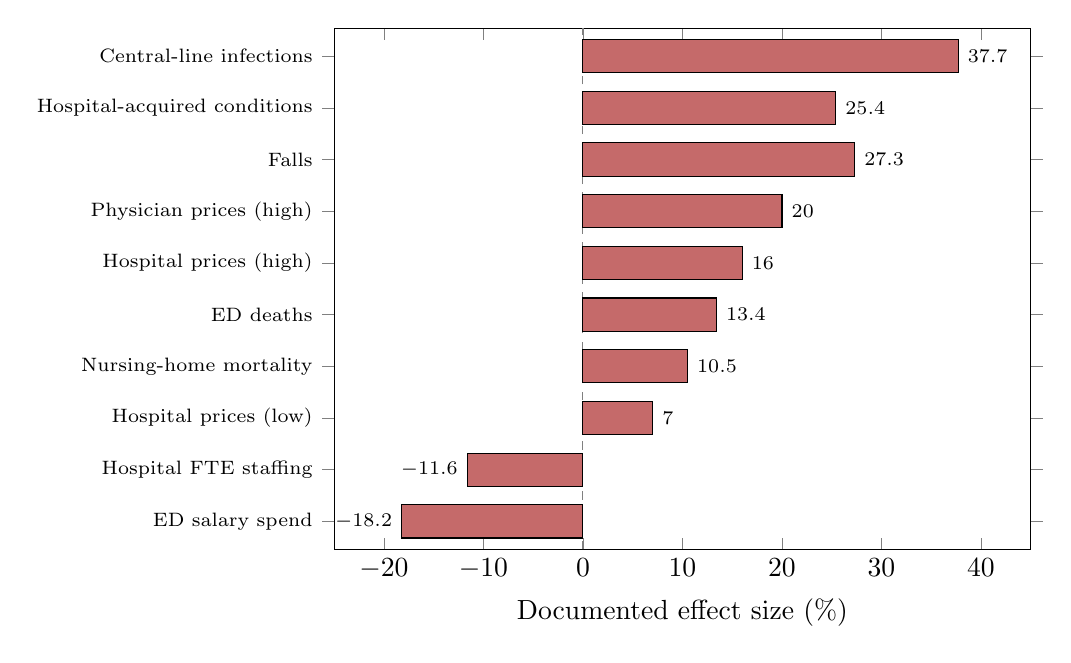
\begin{tikzpicture}
\begin{axis}[
  width=0.86\textwidth, height=8.2cm,
  xbar, bar width=12pt,
  xmin=-25, xmax=45,
  xlabel={Documented effect size (\%)},
  symbolic y coords={EDsalary,FTEstaffing,HospPriceLow,NHmortality,EDdeaths,HospPriceHigh,PhysPriceHigh,Falls,HACs,CLABSI},
  ytick=data,
  yticklabels={ED salary spend,Hospital FTE staffing,Hospital prices (low),Nursing-home mortality,ED deaths,Hospital prices (high),Physician prices (high),Falls,Hospital-acquired conditions,Central-line infections},
  y tick label style={font=\scriptsize},
  nodes near coords, nodes near coords style={font=\scriptsize},
  enlarge y limits=0.06,
  extra x ticks={0}, extra x tick labels={}, extra x tick style={grid=major,grid style={gray,dashed}},
]
\addplot[fill=uccol!65] coordinates {
  (-18.2,EDsalary) (-11.6,FTEstaffing)
  (7,HospPriceLow) (10.5,NHmortality)
  (13.4,EDdeaths) (16,HospPriceHigh)
  (20,PhysPriceHigh) (27.3,Falls)
  (25.4,HACs) (37.7,CLABSI)};
\end{axis}
\end{tikzpicture}
\caption{US private-equity healthcare: documented effect sizes (\%). Negative bars (staffing $-$11.6\%, ED salary $-$18.2\%) denote reductions. \textit{Source:} \cs{S28}; \cs{S49}; \cs{S206}; \cs{S207}.}
\label{fig:ch9effects}
\end{figure}

\textbf{Lesson for India:} demand staffing/infection/pricing/billing metrics post-acquisition; watch sale-leaseback/OpCo-PropCo structures; apply \emph{local-market} roll-up tests below CCI thresholds; adopt pre-close-notice and ownership-transparency tools.

\subsection{United Kingdom and Europe}

\SE\ A $\sim$20-year financialisation experiment produced repeated, regulator-resistant failures: \textbf{Southern Cross} care-home collapse (2011, sale-leaseback under Blackstone-era ownership); \textbf{Four Seasons Health Care} collapse (2019); the \textbf{Orpea/Emeis} France scandal (2022, fraud/abuse, near-collapse); the UK \textbf{CMA} found \textbf{HCA dominant in central London ($\sim$55\% of consulting rooms)} but ultimately \emph{retreated from structural divestiture}; \textbf{BMI Healthcare} opco/propco collapse; \textbf{Circle/Hinchingbrooke} (first private-run NHS hospital, abandoned mid-contract as the CQC rated it ``Inadequate'') \cs{S64}; \cs{S65}; \cs{S224}. \textbf{Two live India links:} Narayana Health bought UK's \textbf{Practice Plus} hospitals (Oct 2025, GBP 188.78m), and \textbf{Circle Health is now owned by Abu Dhabi's PureHealth (ADQ-IHC)} from Centene (US\$1.2bn, 2024) --- the sovereign-cross-border pattern relevant to India. Continent-wide academic finding: PE/for-profit ownership is associated with measurably lower care quality (Sweden JPART \cs{S50}; WHO European Observatory \cs{S52}).

\textbf{Lesson for India:} once frail-elder/acute care is owned through leveraged, offshore, yield-seeking vehicles, the failure modes are predictable and repeating; PPP/managed-hospital contracts need enforceable financial, quality and step-in protections.

\subsection{Food and Grocery}

\SE\ Outcomes are mixed and chain-specific: the US \textbf{FTC $+$ state courts blocked Kroger-Albertsons (Dec 2024)} over prices, wages and competition; Safeway-Albertsons evidence shows upstream specialty-crop grower harm \cs{S88}; UK supermarket LBOs (Asda/TDR-Issa; Morrisons/CD\&R) loaded debt; NBER consumer-goods evidence finds PE raises product-line prices $\sim$5\% (but same-SKU much less --- mix/geography effects) \cs{S83}; \cs{S84}; restaurant-chain PE shows \emph{improved} inspections and \emph{lower} menu prices alongside lower headcount \cs{S86}; OECD cautions that food-chain margin/pass-through claims require chain-specific data \cs{S87}; \cs{S225}; \cs{D:intl\_food\_grocery\_deep}. \textbf{Lesson for India:} food-system claims need SKU-level prices, pack-size, nutrition panels, city/channel shares and farmgate/contract data --- ownership change alone proves nothing.

\subsection{Other comparators}

Australia (rising PE in GP/imaging/ophthalmology \cs{S51}); Canada (for-profit/financialized LTC linked to higher COVID mortality \cs{S67}; \cs{S68}); Brazil (Carlyle/Rede D'Or capacity expansion --- the benefit side \cs{S66}); Chile (FNE \emph{blocked} Isapre Colmena health-insurance merger over price effects \cs{S69}); DFI/Oxfam concerns on for-profit hospital support \cs{S30}. \textbf{Transferability warning:} India's payer mix, OOPE burden, public capacity, price controls and CCI structure differ; international evidence is a risk signal, not a substitute for Indian data \cs{S49}--\cs{S52}; \cs{S64}--\cs{S69}.

% =====================================================================
\section{Causal Analysis --- Correlation vs Causation}\label{sec:causal}
% =====================================================================
\textbf{Why the capital came (\SE).} Under-bedded markets (NITI: 1.3 beds/1{,}000; 3M-bed gap), rising incomes and insurance, fragmented providers ripe for roll-up, export-oriented pharma/CDMO dollar revenues, defensive-growth food/seed assets, a permissive FDI regime (hospitals/devices 100\% automatic), policy support (PLI, PMKSY, \S35AD, SEBI AIF, GIFT-City), and near-zero exit-tax treaty routing. Demand and policy \emph{enabled} the capital; they did not by themselves cause any specific transaction (which also needed promoter willingness, exit paths, and sponsor fundraising cycles).

\textbf{Did consolidation alter behaviour? (\PH.)} Torrent-JB shows CCI sees product-level pharma risk; AHH/GIC's cross-vertical single-specialty platform and metro hospital concentration plausibly confer pricing/bargaining power locally. But the binding test --- \emph{city/specialty market power and before/after pricing at PE-acquired assets} --- has no public dataset.

\textbf{PE ownership or broader industry trends? (\EI.)} Corporate-hospital overcharging, branded-drug markups, diagnostics incentives, supplier-induced demand, medical inflation and public-sector undercapacity \emph{predate} most PE transactions and persist where PE has exited (Max's sector-high ARPOB under founder control). PE can \emph{amplify} these incentives --- and international evidence shows it often does --- but proving India-specific amplification requires matched before/after ownership studies that do not yet exist. \textbf{The honest causal statement: foreign capital is a powerful enabler and accelerant of an organized-tier consolidation whose harms are, so far, demonstrable at the corporate-sector level but not isolated to PE/foreign ownership in India.}

% =====================================================================
\section{Future Scenarios (2026--2041)}\label{sec:scenarios}
% =====================================================================
\begin{itemize}[leftmargin=1.4em,itemsep=3pt]
\item \textbf{Best case (Likelihood 25--35\%).} Capital expands beds, devices, oncology, fertility, pharma manufacturing and cold chain; India adds ownership transparency, healthcare-specific transaction review, local-concentration tests, PM-JAY participation conditions, ARPOB/billing transparency, value-extraction monitoring, and stronger public health spending. Net: capacity, technology and professional management gains with contained concentration/affordability risk.
\item \textbf{Base case (Likelihood 45--55\%).} Consolidation continues (hospitals, single-specialty, CDMO, packaged food, TPAs); regulation stays mostly competition-law-based with incremental disclosure; access expands in profitable urban/Tier-2-3 markets; affordability pressure persists for the uninsured; sovereign capital (Temasek/GIC/Gulf) deepens; food/quick-commerce effects remain mixed and hard to detect.
\item \textbf{Worst case (Likelihood 15--25\%).} Local/specialty roll-ups (oncology, fertility, dialysis, metro multi-specialty) reach pricing power; the TPA claims layer concentrates further; value-extraction tools (debt, leases, fees, dividend recaps, sale-leaseback/REITs) migrate to India as they have elsewhere; PM-JAY participation stays weak; quick-commerce/food concentration raises consumer prices or erodes quality without farmer gains. Plausible from international analogues; \textbf{not currently proven in India.}
\end{itemize}

% =====================================================================
\section{Recommendations}\label{sec:recommendations}
% =====================================================================
\begin{enumerate}[leftmargin=1.6em,itemsep=3pt]
\item \textbf{Healthcare-specific transaction review} (beyond CCI's turnover thresholds) for hospital, diagnostics, oncology, fertility, dialysis, maternity and emergency-care platforms above defined thresholds, with explicit \textbf{local-market (city/specialty) and serial-roll-up} tests.
\item \textbf{Ultimate beneficial-ownership disclosure} for hospitals, diagnostics chains and PM-JAY-empanelled providers (leveraging the SEBI FPI BO regime), piercing Singapore/Mauritius/Cyprus/Netherlands vehicles.
\item \textbf{Mandatory chain/facility disclosure} of beds, specialty mix, ARPOB, payer mix, PM-JAY participation, claim-denial rates, staffing ratios, hospital-acquired-infection rates and adverse events --- pre- and post-acquisition.
\item \textbf{Value-extraction monitoring:} related-party, lease/sale-leaseback, debt, management-fee, dividend-recap and offshore-routing disclosure for providers above size thresholds; pre-emptive limits on hospital-REIT/OpCo-PropCo structures (per the Massachusetts/Steward lesson).
\item \textbf{TPA-layer oversight:} treat the claims-administration tier (Medi Assist-dominated, CR4 $\sim$68\%) as a distinct concentration and conflict-of-interest concern; require claim-adjudication transparency.
\item \textbf{A national hospital pricing/billing-transparency dataset} (consumables, diagnostics, procedures) to enable before/after-ownership and PE-vs-non-PE studies --- closing the single biggest evidentiary gap.
\item \textbf{Condition DFI/public financing and PM-JAY empanelment} on access, emergency-care, price and quality commitments.
\item \textbf{Food/agri:} track category-level concentration, price-pack/portion changes, sodium/sugar/fat reformulation, marketing-to-children, quick-commerce channel dependence; revive FSSAI front-of-pack warning labels; build crop-wise farmgate/contract panels before any farmer-harm finding.
\item \textbf{Conflict-of-interest and lobbying transparency:} disclosure for advisory councils/committees seating regulated industry; a cooling-off framework for regulators (the Wadhawan-type interlock).
\item \textbf{Correct the public debate:} separate verified ownership facts (foreign sovereign $+$ PE capital is structurally central) from unproven claims (national takeover, corruption, PE-specific price/nutrition/farmer causation).
\end{enumerate}

% =====================================================================
\section{Master Findings Classification}\label{sec:findings}
% =====================================================================
\begin{small}
\setlength{\tabcolsep}{4pt}
\begin{longtable}{>{\raggedright\arraybackslash}p{12.0cm} >{\raggedright\arraybackslash}p{3.2cm}}
\caption{Master findings classification.}\label{tab:findings}\\
\toprule
\textbf{Finding} & \textbf{Classification} \\
\midrule
\endfirsthead
\toprule
\textbf{Finding} & \textbf{Classification} \\
\midrule
\endhead
\midrule \multicolumn{2}{r}{\footnotesize\itshape continued on next page}\\
\endfoot
\bottomrule
\endlastfoot
Foreign PE/sovereign/institutional capital holds structurally central positions in India's organized healthcare, pharma, medtech, packaged-food, quick-commerce and seeds tiers. & VERIFIED FACT \\
IHH (Malaysia/Mitsui/Khazanah) is the largest foreign-\emph{control} hospital position (Fortis 31.17\% promoter $+$ 100\% Gleneagles); its Nov-2025 open offer drew near-zero acceptance, so it did \textbf{not} reach majority. & VERIFIED FACT \\
Sovereign/pension capital (esp. Temasek/GIC) --- not US buyout PE alone --- is the centre of gravity; much US-PE hospital entry has already exited via IPO. & STRONG EVIDENCE-BASED CONCLUSION \\
One Singapore-sovereign-controlled platform (AHH/GIC$+$TPG) spans IVF, mother-\&-child and nephro-urology --- the most antitrust-relevant single-specialty concentration. & VERIFIED FACT \\
National hospital/diagnostics concentration is low (organized-pool CR4 $\sim$16--24\%; HHI $<$1{,}000); the diagnostics leader holds $<$6\% nationally. ``Monopolized'' is unsupported nationally. & STRONG EVIDENCE-BASED CONCLUSION \\
``$\approx$25\% of organized beds PE-controlled'' is denominator-dependent: $\sim$36--46\% of the organized large-chain pool (foreign-PE$+$sovereign), but $\sim$1.3--3\% of all-India/all-private beds. & EXPERT INTERPRETATION \\
The aggressive US value-extraction toolkit (REIT sale-leaseback, dividend recaps) is largely latent in India; ARPOB escalation (not PE-specific) is the operative lever; HCG's post-KKR gearing jump is the clearest leverage signal. & STRONG EVIDENCE-BASED CONCLUSION \\
TPA claims layer is highly concentrated (CR4 $\sim$68\%; Medi Assist $\sim$31--37\%) and most foreign-PE-linked; insurance overall is unconcentrated (HHI $\sim$700--830). & VERIFIED FACT / STRONG EVIDENCE-BASED CONCLUSION \\
Foreign capital has disproportionately scaled India's HFSS/UPF food categories amid an exploding metabolic-disease burden. & STRONG EVIDENCE-BASED CONCLUSION \\
FDI regime is permissive and tax/treaty/GIFT-City architecture enables near-zero exit-tax routing (Singapore-dominant post-2017). & VERIFIED FACT \\
Documented influence channels exist (IVCA officered by PE heads; PE-backed chains lead provider associations; AdvaMed$\rightarrow$GSP; industry seated in DoP pricing committee; pharma electoral bonds). & VERIFIED FACT \\
India-specific PE-vs-non-PE causal effect on prices/quality is plausible but \textbf{unproven}; flagship harm incidents pre-date foreign control; harms are corporate-sector-wide. & PLAUSIBLE HYPOTHESIS \\
US/UK/Europe evidence shows real PE-ownership harms (mortality, adverse events, prices, collapses) --- a risk signal, not India proof. & STRONG EVIDENCE-BASED CONCLUSION \\
Food-price, nutrition and farmer-harm causation from PE/institutional ownership in India is \textbf{not proven}. & UNPROVEN CLAIM \\
Regulatory capture (a specific bought policy) is \textbf{not established}, though interlocks and the channels above justify a conflict-of-interest inquiry. & UNPROVEN CLAIM / EXPERT INTERPRETATION \\
A parliamentary/antitrust-grade inquiry into ownership transparency, local concentration, the TPA layer, value extraction and food-sector concentration is justified. & EXPERT INTERPRETATION \\
\end{longtable}
\end{small}

% =====================================================================
\section{Limitations and Residual Gaps}\label{sec:limitations}
% =====================================================================
\begin{itemize}[leftmargin=1.4em,itemsep=2pt]
\item \textbf{No PE-vs-non-PE India outcome dataset} (the single biggest gap); no public city-level hospital CR4/HHI; no ownership-tagged all-private-bed census.
\item \textbf{Private documents not obtained:} shareholder agreements, side letters, reserved-matters/board-rights, fund LP composition, MCA charge filings, deal-level tax routing/treaty application.
\item \textbf{Many deal values are press-reported}, not from filings/CCI orders (flagged throughout); several CCI primary order texts were referenced via summaries, not parsed in full.
\item \textbf{Unverified/forward items:} IHH's stated intent to reach 50\% (not executed); GIC's ``majority'' of AHH (press-reported); Manipal/Haldiram precise valuations (press); Cloudnine stake-sale (in process); the SC-ordered Fortis--IHH forensic audit outcome (not located); Max Shalimar Bagh final licence disposition.
\item \textbf{Corrected brief premises (carried from dossiers):} Veeda $=$ CX Partners (not CVC); Sekhmet $=$ PAG-led (not Advent); Savannah $=$ RiceTec/US (not Bayer); no QIA--Cloudnine link; CPPIB hospital/pharma control unproven; no Bain--Laurus or Sekhmet--Raptakos link.
\item \textbf{Food/agri farmer-impact and nutrition causation} remain hypotheses pending SKU-price, farmgate, reformulation and consumption panels.
\end{itemize}

% =====================================================================
\section{Cumulative FDI Context}\label{sec:fdi}
% =====================================================================
\VF\ Cumulative FDI into relevant sectors (DPIIT FDI Fact Sheet, Apr 2000--Dec 2025) is shown in Table~\ref{tab:fdicum} and Figure~\ref{fig:ch11fdi}. These are sector aggregates, not foreign-PE-only flows.

\begin{table}[htbp]
\centering
\small
\caption{Cumulative FDI inflows relevant to this investigation (Apr 2000--Dec 2025). \textit{Source:} DPIIT FDI Fact Sheet, \cs{S03}.}
\label{tab:fdicum}
\begin{tabularx}{\textwidth}{@{}>{\raggedright\arraybackslash}X r r r@{}}
\toprule
\textbf{Sector} & \textbf{INR crore} & \textbf{US\$ million} & \textbf{\% of total FDI equity} \\
\midrule
Drugs and Pharmaceuticals & 154{,}388.59 & 24{,}812.83 & 3.19\% \\
Food Processing Industries & 110{,}459.97 & 15{,}856.23 & 2.04\% \\
Hospital and Diagnostic Centres & 90{,}215.67 & 12{,}726.93 & 1.64\% \\
Medical and Surgical Appliances & 30{,}402.49 & 4{,}247.91 & $\sim$0.55\% \\
Agriculture Services & 26{,}443.47 & 3{,}979.17 & $\sim$0.51\% \\
\bottomrule
\end{tabularx}
\end{table}

% ---- FIGURE: CH11 cumulative FDI ----
\begin{figure}[htbp]
\centering
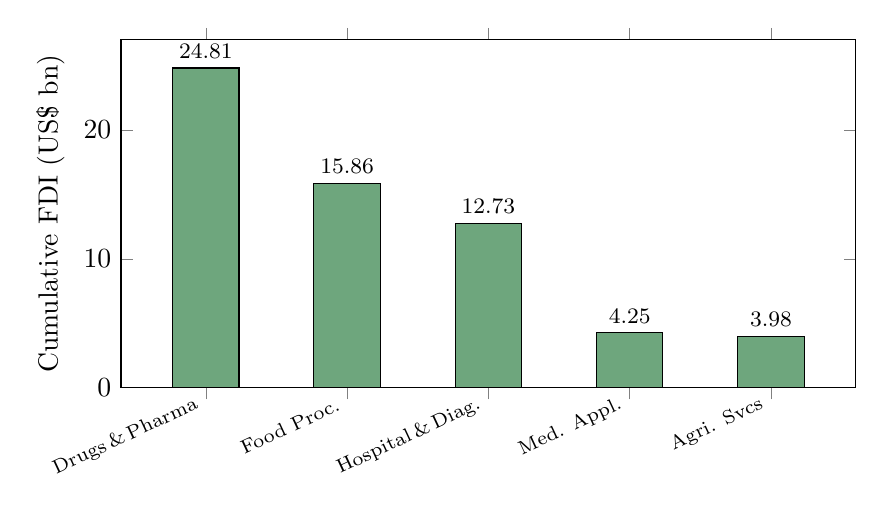
\begin{tikzpicture}
\begin{axis}[
  width=0.90\textwidth, height=6.0cm,
  ybar, bar width=24pt,
  ymin=0, ymax=27,
  ylabel={Cumulative FDI (US\$ bn)},
  symbolic x coords={DrugsPharma,FoodProc,HospitalDiag,MedAppl,AgriSvcs},
  xtick=data,
  xticklabels={Drugs\,\&\,Pharma,Food Proc.,Hospital\,\&\,Diag.,Med. Appl.,Agri. Svcs},
  x tick label style={rotate=25,anchor=east,font=\scriptsize},
  nodes near coords, nodes near coords style={font=\footnotesize},
  enlarge x limits=0.15,
]
\addplot[fill=vfcol!60] coordinates {(DrugsPharma,24.81) (FoodProc,15.86) (HospitalDiag,12.73) (MedAppl,4.25) (AgriSvcs,3.98)};
\end{axis}
\end{tikzpicture}
\caption{Cumulative FDI into relevant sectors, Apr 2000--Dec 2025 (US\$ bn). \textit{Source:} DPIIT, \cs{S03}.}
\label{fig:ch11fdi}
\end{figure}

% =====================================================================
\section{Expanded Major-Transactions Database (Selected New \& Updated Entries)}\label{sec:transactions}
% =====================================================================
This consolidates the most material \emph{new} verified/strong transactions added in this edition. Values marked ``press'' are press-reported; stakes from filings/CCI/company releases are ``official.''

\begin{landscape}
\begin{footnotesize}
\setlength{\tabcolsep}{3pt}
\renewcommand{\arraystretch}{1.1}
\begin{longtable}{>{\raggedright\arraybackslash}p{1.6cm} >{\raggedright\arraybackslash}p{2.9cm} >{\raggedright\arraybackslash}p{2.6cm} >{\raggedright\arraybackslash}p{2.0cm} >{\raggedright\arraybackslash}p{2.6cm} >{\raggedright\arraybackslash}p{3.0cm} >{\raggedright\arraybackslash}p{2.6cm} >{\raggedright\arraybackslash}p{1.4cm}}
\caption{Expanded major-transactions database: selected new and updated entries. \textit{Source:} \texttt{major\_transactions.csv}; per-deal URL trails in the dossiers.}\label{tab:transactions}\\
\toprule
\textbf{Date} & \textbf{Investor (ultimate)} & \textbf{Target} & \textbf{Sector} & \textbf{Value} & \textbf{Stake/Control} & \textbf{Vehicle/Juris.} & \textbf{Class.} \\
\midrule
\endfirsthead
\toprule
\textbf{Date} & \textbf{Investor (ultimate)} & \textbf{Target} & \textbf{Sector} & \textbf{Value} & \textbf{Stake/Control} & \textbf{Vehicle/Juris.} & \textbf{Class.} \\
\midrule
\endhead
\midrule \multicolumn{8}{r}{\footnotesize\itshape continued on next page}\\
\endfoot
\bottomrule
\endlastfoot
Nov 2018 & IHH Healthcare (Malaysia; Mitsui/Khazanah) & Fortis Healthcare & Hospitals & $\sim$Rs 4{,}000 cr @Rs 170 (official) & 31.1\% promoter; open offer failed Nov 2025 (stays 31.17\%) & Northern TK Venture (Singapore) & VERIFIED \\
2023 (100\%) & IHH Healthcare & Gleneagles Healthcare India & Hospitals & $\sim$Rs 740 cr (press) & 100\% & Gleneagles Development (India) & VERIFIED \\
Aug--Dec 2024 & Fortis (IHH) buys out IFC/Jacob Ballas/Avigo & Agilus Diagnostics & Diagnostics & $\sim$Rs 1{,}780 cr for 31.52\% (press) & $\rightarrow$89.2\%$\rightarrow$$\sim$100\% & Fortis (India) & VERIFIED \\
2023 & Blackstone (US) $+$ TPG & Quality Care India (CARE/KIMS Health) & Hospitals & $\sim$US\$1bn (press) & Blackstone $\sim$72.5\%, TPG $\sim$27.5\% & BCP Asia II Topco IV (SG); Centella (Mauritius) & VERIFIED \\
Nov 2024 & Blackstone $+$ Aster founders & Aster DM Quality Care merger & Hospitals & EV $\sim$US\$5bn (press) & Blackstone 30.7\%, joint control; NCLT pending & Singapore/Mauritius & STRONG \\
Feb 2023 & Temasek (Singapore SWF) & Manipal Health Enterprises & Hospitals & $+$41\%, $\sim$US\$2bn (press) & $\rightarrow$$\sim$59\% control & Sheares Healthcare (Singapore) & VERIFIED (stake) \\
Feb 2024 & Mubadala $+$ Novo Holdings $+$ CalPERS & Manipal Health Enterprises & Hospitals & undisclosed & 8\% combined & UAE/Denmark/US & VERIFIED \\
Jul 2025 & Manipal (Temasek) $\leftarrow$ OTPP (Canada) & Sahyadri Hospitals & Hospitals & $\sim$Rs 5{,}800 cr (press) & control transfer (sovereign$\leftrightarrow$pension) & India & STRONG \\
Feb 2025 & KKR (US) $\leftarrow$ CVC & HCG (oncology) & Hospitals & up to $\sim$US\$400m & 54.27\% (sole control) & Hector Asia Holdings II (Singapore) & VERIFIED \\
2022--24 & GIC (Singapore SWF) & Asia Healthcare Holdings (Nova IVF/Motherhood/AINU) & Single-specialty & US\$320m & control/anchor & Singapore & VERIFIED \\
2023 & BPEA EQT & Indira IVF & Fertility & $\sim$Rs 6{,}000 cr/$\sim$US\$1.1bn (press) & $\sim$60\% control (ex-TA Associates) & BPEA PE Fund VIII & VERIFIED (control) \\
2022 & General Atlantic $+$ Kedaara & ASG Eye Hospitals & Eye care & Rs 1{,}500 cr & $\sim$46\% (ex-Investcorp) & --- & VERIFIED \\
Feb 2025 & TPG $+$ Temasek (OFS) & Dr Agarwal's Health Care (IPO) & Eye care & $\sim$Rs 3{,}027 cr issue & TPG 33.75\%/Temasek 28.18\% pre-IPO & Hyperion/Arvon (SG); Claymore (Mauritius) & VERIFIED \\
Dec 2025 & Quadria (Singapore) & NephroPlus (IPO) & Dialysis & Rs 490 issue & $\sim$30\% largest holder & Quadria (Singapore) & VERIFIED \\
Dec 2022$\rightarrow$2025 & Advent (US) & Suven Pharmaceuticals $\rightarrow$ Cohance & CDMO/API & Rs 495/sh; FDI $\le$Rs 9{,}589 cr & 50.1\%$\rightarrow$$\sim$76\% & Berhyanda (Cyprus) & VERIFIED \\
2018$\rightarrow$2025 & TPG (US) & Sai Life Sciences & CRDMO & IPO Rs 3{,}043 cr & $\sim$39\%$\rightarrow$full exit Aug 2025 & TPG Asia VII SF (Singapore) & VERIFIED \\
May 2021 & Goldman Sachs (US) & Aragen (ex-GVK Bio) & CRDMO & $\sim$US\$1bn valn & $\sim$one-third (ChrysCap exit) & offshore & VERIFIED \\
2022 / 2025 & ChrysCap $+$ Temasek; Goldman/ADQ/Viatris & Intas; Biocon Biologics & Pharma/biosimilars & various & foreign minorities & Singapore/UAE/US & VERIFIED \\
Mar 2021 / Jul 2025 & Warburg Pincus (NL) $+$ ADIA (Abu Dhabi) & Meril / Micro Life Sciences & Medical devices & WP $\sim$US\$210m; ADIA $\sim$US\$200m (EV $\sim$US\$6.6bn) & $\sim$13\% $+$ $\sim$3\% & South Elm (NL); Platinum (Abu Dhabi) & VERIFIED \\
May 2024 & KKR (US) $\leftarrow$ Apax & Healthium MedTech & Medical devices & $\sim$US\$839m (press) & control & KKR Asian Fund IV & VERIFIED \\
2024 & Advent (US) & Apollo HealthCo $+$ Keimed & Pharmacy/distribution & Rs 2{,}475 cr & 12.1\% (AHEL $\ge$59.2\%) & Rasmeli (Advent) & VERIFIED \\
Jan 2024 (IPO) & Bessemer (US) $+$ Investcorp (Gulf) $\rightarrow$ Novo (DK) & Medi Assist (TPA) & TPA & OFS & $\sim$45\%/$\sim$21\% sold down & offshore & VERIFIED \\
Aug 2024 & Medi Assist $\leftarrow$ Fairfax (Canada) & Paramount Health TPA & TPA & $\sim$Rs 311 cr (press) & 100\% & India/Canada & VERIFIED \\
2024 & Bupa (UK); ADIA & Niva Bupa; Aditya Birla Health & Insurance & --- & $\sim$63\%; 10\% & Bupa Singapore; Abu Dhabi & VERIFIED \\
2024--25 & Temasek; IHC $+$ Alpha Wave & Haldiram Snacks Food & Packaged food & $\sim$US\$10bn valn (press) & $\sim$10\%; $\sim$6\% & Jongsong (SG); UAE/US & VERIFIED (CCI stakes) \\
Mar 2026 & General Atlantic & Balaji Wafers & Packaged snacks & 6.93\% (official) & minority & GA Singapore BWP & VERIFIED \\
Aug 2025 & ChrysCapital & Theobroma Foods & Bakery/F\&B & --- & $\sim$84\% control & Aqua (Mauritius)/Atreides (NL) & VERIFIED \\
Jan 2024 & Khazanah (Malaysia SWF) & Wow! Momo & QSR & Rs 350 cr & $\sim$15\% & Malaysia & STRONG \\
Oct 2025 & CalPERS (US pension) & Zepto & Quick commerce & $\sim$US\$450m @ US\$7bn (press) & lead minority & US & STRONG \\
2022 / 2024 & KKR (US); Alpha Wave & Advanta (UPL seeds) & Seeds & US\$300m; US\$350m & $\sim$13.3\%; $\sim$12.5\% & KKR Global Impact; Alpha Wave & STRONG \\
2015 & Fairfax India (Canada) & NCML (grain handling) & Agri-warehousing & $\sim$Rs 800 cr & $\sim$74\% control & Fairfax India (Canada) & VERIFIED \\
\end{longtable}
\end{footnotesize}
\end{landscape}

% =====================================================================
\appendix
\section{Sources Register (Bibliography)}\label{app:sources}
% =====================================================================
This appendix is the bibliography. Every \cs{Sxx} citation in the body maps to a row here. Reliability codes (where used in the June 2026 addendum): P $=$ primary/official/filing; C $=$ company/investor release; M $=$ market-research/ratings; A $=$ academic/peer-reviewed; J $=$ high-quality press. Long ``used-for'' notes are abbreviated. URLs are rendered with \texttt{\textbackslash url} and are click-through in the PDF.

\begin{footnotesize}
\setlength{\tabcolsep}{3pt}
\renewcommand{\arraystretch}{1.12}
\begin{longtable}{>{\raggedright\arraybackslash}p{0.9cm} >{\raggedright\arraybackslash}p{3.4cm} >{\raggedright\arraybackslash}p{1.6cm} >{\raggedright\arraybackslash}p{2.0cm} >{\raggedright\arraybackslash}p{3.6cm} >{\raggedright\arraybackslash}p{3.1cm}}
\caption{Sources register (S01--S228 and repository artifacts L01--L07).}\label{tab:sources}\\
\toprule
\textbf{ID} & \textbf{Source / title} & \textbf{Date} & \textbf{Reliability} & \textbf{Used for} & \textbf{URL} \\
\midrule
\endfirsthead
\toprule
\textbf{ID} & \textbf{Source / title} & \textbf{Date} & \textbf{Reliability} & \textbf{Used for} & \textbf{URL} \\
\midrule
\endhead
\midrule \multicolumn{6}{r}{\footnotesize\itshape continued on next page}\\
\endfoot
\bottomrule
\endlastfoot
L01 & report.pdf converted to text & 2026-06-03 & Low as evidence; high as repository claim inventory & Local generated report claims and chart captions & (local/no public URL) \\
L02 & Kimi Chinese archive report.md & 2026-06-03 & Low as evidence; high as repository claim inventory & Local generated report claims, scenario claims, chart references & (local/no public URL) \\
L03 & Kimi US final\_report\_us\_pe\_india.md & 2026-06-03 & Low as evidence; high as repository claim inventory & Local generated timeline and transaction claims & (local/no public URL) \\
L04 & government\_corruption\_report.md & 2026-06-03 & Low for allegations; useful for claim leads & Policy, corruption, overcharging, and prescribing allegations requiring verification & (local/no public URL) \\
L05 & us\_pe\_india\_healthcare\_food\_report.md & 2026-06-03 & Low as evidence; high as repository claim inventory & 2020-2026 transaction claim list & (local/no public URL) \\
L06 & us\_pe\_report\_zip markdown report & 2026-06-03 & Low as evidence; high as repository claim inventory & Duplicate/variant generated report & (local/no public URL) \\
L07 & Generated chart images & 2026-06-03 & Low unless underlying data verified & Infographic claim inventory & (local/no public URL) \\
S01 & DPIIT Consolidated FDI Policy Circular of 2020 & 2020-10-15 & High & FDI routes for manufacturing, food-product retail, pharma, medical devices & \url{https://www.dpiit.gov.in/static/uploads/2025/07/edd58e9c254bfbddc418f7059165a991.pdf} \\
S02 & DPIIT sectors under automatic route & 2025 archive & High & Automatic-route sector verification & \url{https://www.dpiit.gov.in/static/uploads/2025/07/7d762b696010fb7efc6da89ab4c510e4.pdf} \\
S03 & DPIIT FDI Fact Sheet December 2025 & 2025-12 & High & Cumulative FDI inflows by sector through December 2025 & \url{https://www.dpiit.gov.in/static/uploads/2026/02/6dc3e8a9fe52d5a412d8e5f41d7b921f.pdf} \\
S04 & DPIIT clarification on Food Product Retail Trading & 2018 & High & Food-product retail trading under government approval route & \url{https://www.dpiit.gov.in/static/uploads/2025/07/95d836222f2c740ec416d73551351734.pdf} \\
S05 & NITI Aayog Investment Opportunities in India's Healthcare Sector & 2021; hosted 2023 & Medium-high; official investment-promotion document & Healthcare FDI routes, bed gap, hospital infrastructure opportunity, tax incentives & \url{https://www.niti.gov.in/sites/default/files/2023-02/InvestmentOpportunities_HealthcareSector.pdf} \\
S06 & National Health Policy 2017 & 2017 & High for policy text & Public spending target, private-sector alignment, regulation, catastrophic expenditure goals & \url{https://extranet.who.int/cpcd/sites/default/files/public_file_repository/IND_India_National-Health-Policy_2017.pdf} \\
S07 & PIB release on National Health Policy 2017 & 2018-01-02 & High & Confirmation of 2.5\% GDP public health expenditure target & \url{https://www.pib.gov.in/newsite/printrelease.aspx?relid=175107} \\
S08 & PIB/MoHFW National Health Accounts 2022-23 & 2026-05-27 & High & Latest official OOPE, GHE/THE, and GHE/GDP values & \url{https://www.pib.gov.in/PressReleasePage.aspx?PRID=2265816&lang=1&reg=1} \\
S09 & EY Private Equity and Venture Capital Trendbook 2025 & 2025 & Medium-high; industry source & India PE/VC 2024 totals, life sciences investment, buyouts, exits & \url{https://www.ey.com/content/dam/ey-unified-site/ey-com/en-in/insights/private-equity/documents/ey-private-equity-and-venture-capital-trendbook-2025-v1.pdf} \\
S10 & Aster DM, BCP Asia, Centella, and QCIL combination approval & 2025-04-15 & High & Aster-QCIL parties, Blackstone/TPG links, QCIL network & \url{https://www.pib.gov.in/PressReleasePage.aspx?PRID=2121949} \\
S11 & Aster and Blackstone-backed Quality Care merger announcement & 2024-11-29 & Medium-high; self-interested company source & Aster-QCIL merger structure, expected bed count and ownership & \url{https://www.asterdmhealthcare.in/newsroom/detail/aster-and-blackstone-backed-quality-care-have-merged-establish-one-of-top-3-hospital-chains-india} \\
S12 & Aster DM Healthcare Q3 FY26 investor presentation & 2026-01-30 & Medium-high; company filing & Aster-QCIL expected completion status and pipeline beds & \url{https://www.asterdmhealthcare.in/fileadmin/InvestorspresentationQ3FY202526.pdf} \\
S13 & KKR-HCG combination approval & 2025-05-01 & High & KKR/Hector acquisition up to 54\%, open offer, expected stake range & \url{https://www.cci.gov.in/public/images/pressrelease/en/press-release1746101546.pdf} \\
S14 & HCG press release on KKR acquisition & 2025-02-23 & High for announcement & HCG deal terms and KKR operational-control intent & \url{https://nsearchives.nseindia.com/corporate/HCG1_23022025220307_SE_Intimation_-_Press_Release_23_February_2025.pdf} \\
S15 & Torrent-JB Chemicals order with voluntary modifications & 2025-10-21 & High & Pharma concentration assessment and remedies & \url{https://www.cci.gov.in/public/images/caseorders/en/order1770108518.pdf} \\
S16 & Torrent to acquire controlling stake in JB Chemicals from KKR & 2025-06-29 & Medium-high; company source & Deal value and transaction structure & \url{https://www.businesswire.com/news/home/20250629033492/en/Torrent-Pharma-to-Acquire-Controlling-Stake-in-J.-B.-Chemicals-Pharmaceuticals-from-KKR} \\
S17 & Temasek/Jongsong-Haldiram approval & 2025-05-20 & High & Less-than-10\% Haldiram acquisition, Temasek link & \url{https://www.cci.gov.in/public/images/pressrelease/en/press-release1747744892.pdf} \\
S18 & Alpha Wave/IHC-Haldiram order & 2025-06-24 & High & 6\% Haldiram stake, ownership links, packaged-food overlaps & \url{https://www.cci.gov.in/images/caseorders/en/order1754894588.pdf} \\
S19 & L Catterton-Haldiram order & 2026-02-03 & High & L Catterton AIF, advisory agreement, Haldiram channels and overlap assessment & \url{https://www.cci.gov.in/images/caseorders/en/order1778136763.pdf} \\
S20 & Carlyle and Piramal Pharma agreement & 2020-06-27 & Medium-high; company/PE source & US\$490M investment for 20\% stake & \url{https://www.carlyle.com/media-room/news-release-archive/carlyle-and-piramal-pharma-sign-agreement-20-strategic-growth} \\
S21 & Manipal Health Enterprises and Temasek transaction & 2023-04-10 & Medium-high; company source & Temasek 41\% additional stake, TPG 11\%, Manipal Group 30\%, Sheares 18\% & \url{https://www.manipalhospitals.com/uploads/press_releases/press_pdf/2__Press_Release_Manipal_Health_Enterprises_announces_agreement_for_Temasek_to_acquire_41_stake_April_10_2023.pdf} \\
S22 & KKR to acquire Healthium from Apax funds & 2024-05-06 & Medium-high; seller source & Healthium controlling-interest transfer & \url{https://www.apax.com/news-views/kkr-to-acquire-healthium-from-apax-funds/} \\
S23 & Mankind to acquire Bharat Serums from Advent & 2024-07-25 and 2024-10-23 & Medium-high; company source & BSV acquisition signing and Advent exit & \url{https://www.mankindpharma.com/media/press-release/mankind-pharma-to-acquire-bharat-serums-from-advent-international-for-rs-13630-cr/} \\
S24 & KKR acquires controlling stake in Baby Memorial Hospital & 2024-07-01 & Medium; press-release mirror & BMH controlling-stake announcement & \url{https://markets.financialcontent.com/stocks/article/bizwire-2024-7-1-kkr-acquires-controlling-stake-in-baby-memorial-hospital-a-multi-specialty-hospital-network-in-india} \\
S25 & Tata Consumer Products to acquire Capital Foods & 2024-01-12 & Medium-high; company source & Capital Foods strategic exit and PE-backed investor history & \url{https://www.tataconsumer.com/news/tata-consumer-products-acquire-capital-foods-owner-chings-secret-and-smith-jones-brands} \\
S26 & UPL Advanta Alpha Wave investment & 2024-11-19 & Medium-high; company source & US\$350M Alpha Wave investment for approx. 12.5\% of Advanta and prior KKR investment & \url{https://www.upl-ltd.com/shareholdercenter_pdfs/Az5JLmYgTColixj1LMZ4Nd0USGiX2AK10lc6NeV7/UPLAWPress-Release.pdf} \\
S27 & Evaluating trends in private equity ownership and impacts on health outcomes, costs, and quality & 2023 & High for international evidence & International PE-healthcare impact evidence & \url{https://www.bmj.com/content/382/bmj-2023-075244} \\
S28 & Changes in Hospital Adverse Events and Patient Outcomes Associated With Private Equity Acquisition & 2023 & High for US hospital evidence & US hospital adverse-event evidence & \url{https://jamanetwork.com/journals/jama/fullarticle/2813379} \\
S29 & Financialisation and the Reshaping of Private Healthcare: A Case Study in India & 2025 & High for qualitative India mechanism evidence; not a quantitative causal estimate & India-specific qualitative study using policy documents, witness seminars and interviews in Maharashtra. It argues that financialisation has facilitated restructuring toward corporate chains and calculative logics, wi... & \url{https://pmc.ncbi.nlm.nih.gov/articles/PMC12082753/} \\
S30 & Oxfam Sick Development report & 2023-06-29 & Medium; advocacy source with methods/data & DFI/private hospital harm allegations and dataset & \url{https://policy-practice.oxfam.org/resources/sick-development-how-rich-country-government-and-world-bank-funding-to-for-prof-621529/} \\
S31 & NPPA Fortis dengue patient medicines and consumables tables & 2017-12-15 archive entry & High for regulator table provenance; PDF contains table data rather than a full adjudicatory order & Corporate hospital billing-rate/procurement-margin evidence: scheduled formulations up to 343\%, non-scheduled formulations up to 914\%, and consumables up to 1,737\% in the Fortis Memorial Research Institute Gurgaon den... & \url{https://nppa.gov.in/archive_2017} \\
S32 & Warburg Pincus enhances stake in Max Healthcare & 2005 & Medium-high; company release & Warburg Pincus Rs 140 crore Max Healthcare investment for 23\% fully diluted stake and Rs 340 crore group exposure & \url{https://www.maxindia.com/mediadetails/warburgpincusenhances} \\
S33 & Apax Apollo Hospitals portfolio page & 2007 investment; realised & Medium; PE portfolio page & Apax investment year, realised status, Apollo hospital/pharmacy/diagnostics/insurance footprint & \url{https://www.apax.com/partnerships/apollo-hospitals/} \\
S34 & TPG to invest in Manipal Health Enterprises & 2015-02-26 & Medium-high; PE/company release & TPG Rs 900 crore significant minority investment in Manipal & \url{https://www.tpg.com/news-and-insights/tpg-invest-manipal-health-enterprises} \\
S35 & Thyrocare detailed public statement for Docon/API Holdings open offer & 2021-07 & High & API/PharmEasy control acquisition of Thyrocare, 66.11\% SPA, 26\% open offer, API foreign institutional shareholders & \url{https://www.sebi.gov.in/sebi_data/commondocs/jul-2021/DPS%20THYROCARE_p.PDF} \\
S36 & Swiggy Limited prospectus & 2024-11-11 & High & Food delivery/quick-commerce institutional ownership, MIH 30.95\%, no identifiable promoter, board nomination rights & \url{https://www.sebi.gov.in/filings/public-issues/nov-2024/swiggy-limited-prospectus_88320.html} \\
S37 & Zomato proposed acquisition of Blinkit & 2022-06-24 & High & Blinkit quick-commerce acquisition rationale, INR 45,082 million consideration, dark-store model & \url{https://archives.nseindia.com/corporate/ZOMATO_24062022195320_Zomato_ProposedAcquisitionofBlinkit.pdf} \\
S38 & Tata Digital acquisition of BigBasket entities & 2021-04-29 & High & CCI approval for up to 64.3\% of Supermarket Grocery Supplies and sole control over Innovative Retail Concepts & \url{https://www.pib.gov.in/PressReleaseIframePage.aspx?PRID=1714774} \\
S39 & Tata Digital logs into BigBasket & 2021-05-28 & Medium-high; company release & BigBasket majority acquisition, food and grocery e-commerce footprint & \url{https://www.tata.com/newsroom/business/tata-digital-bigbasket-acquisition} \\
S40 & Reliance Retail acquisition of METRO Cash \& Carry India & 2022-12-22 & Medium-high; company release & 100\% acquisition, Rs 2,850 crore value, 31 stores, 21 cities, B2B/kirana network & \url{https://www.ril.com/sites/default/files/2023-01/MR22122022-RRVL.pdf} \\
S41 & CCI approval for Reliance-METRO India & 2023-03-14 & High & Competition approval for food/grocery wholesale consolidation & \url{https://www.cci.gov.in/public/images/pressrelease/en/press-release1678856452.pdf} \\
S42 & FSSAI Food Safety and Standards Labelling and Display Regulations 2020, version VIII & 2025-09-09 & High & Current labelling framework for pre-packaged foods; nutrition governance context & \url{https://www.fssai.gov.in/upload/uploadfiles/files/Comp_Labelling%20Display_Version%20VIII_09_09_2025.pdf} \\
S43 & CCI filing of combination notice introduction & 2026 accessed & High & Combination thresholds and March 2024 de-minimis exemption context & \url{https://www.cci.gov.in/public/combination/combination/filing-of-combination-notice/introduction} \\
S44 & Carlyle buys stake in Metropolis Healthcare & 2015-09-09 & Medium-high; PE/company release & Carlyle Asia Partners IV affiliate bought stake in Metropolis; Metropolis had 130 labs and 1,000+ collection centers in India & \url{https://www.carlyle.com/media-room/news-release-archive/carlyle-group-buys-stake-metropolis-healthcare-limited} \\
S45 & WestBridge Dr Lal PathLabs portfolio page & 2005 Series A investment & Medium; PE portfolio page & WestBridge Series A investment and Dr Lal PathLabs scale indicators & \url{https://westbridgecap.com/portfolio/dr-lal-pathlabs} \\
S46 & Agilus Diagnostics investor page & 2025 accessed & Medium-high; company page & Agilus claims largest diagnostic service provider by number of laboratories FY2023 and lists board/investor document categories & \url{https://agilusdiagnostics.com/our-investors} \\
S47 & Star Health and Allied Insurance DRHP & 2021 & High & Health-insurance investor transactions involving WestBridge, Madison, Apis, US entities, Tata Capital and IRDAI approvals & \url{https://www.sbicaps.com/wp-content/uploads/2021/10/Star-Health-and-Allied-Insurance-Company-Limited-DRHP.pdf} \\
S48 & Medi Assist Healthcare Services basis of allotment/public announcement & 2024-01 & High & TPA/health-benefits-administrator IPO offer size and Bessemer/Investcorp selling-shareholder evidence & \url{https://www.mediassist.in/assets/pdf/investor-relations/mahs/ads/basis-of-allotment.pdf} \\
S49 & How Patients Fare When Private Equity Funds Acquire Nursing Homes & 2021-04 & High for US nursing-home evidence summary & Higher mortality, fewer caregiver hours, higher charges, interest and lease-payment mechanisms after PE nursing-home acquisitions & \url{https://www.nber.org/digest/202104/how-patients-fare-when-private-equity-funds-acquire-nursing-homes} \\
S50 & Provider Ownership and Indicators of Service Quality: Evidence from Swedish Residential Care Homes & 2024 & High for Sweden elder-care evidence & Panel evidence on ownership form and quality indicators; PE and publicly traded firms often lower in quality distribution & \url{https://academic.oup.com/jpart/article/34/1/150/7066933} \\
S51 & Private equity investment in health care delivery, Australia, 2008-2022 & 2024 & High for Australian investment-mapping evidence & Rise of PE acquisitions in Australian health care delivery, especially general practice, imaging, ophthalmology & \url{https://www.mja.com.au/journal/2024/220/7/private-equity-investment-health-care-delivery-australia-2008-2022} \\
S52 & Private equity investment in long-term care in Europe: trends, impact and policy options & 2026 & High for comparative policy synthesis & European LTC evidence and policy options, including ownership disclosure and acquisition review & \url{https://eurohealthobservatory.who.int/docs/librariesprovider3/publicationsnew/private-equity-investment-in-long-term-care-2nd-pp.pdf?download=true&sfvrsn=4f1be491_1} \\
S53 & ICMR-NIN Dietary Guidelines for Indians 2024 & 2024 & High & ICMR-NIN estimates that 56.4\% of India's total disease burden is due to unhealthy diets, links unhealthy highly processed HFSS foods with affordability/accessibility and aggressive advertising, and Guideline 15 says t... & \url{https://nin.res.in/dietaryguidelines/pdfjs/locale/DGI_2024.pdf} \\
S54 & The growth of ultra-processed foods in India: an analysis of trends, issues and policy recommendations & 2023-08-22 & High & WHO India analyses five UPF categories: chocolate and sugar confectionery, salty snacks, beverages, ready-made and convenience food, and breakfast cereals. It reports 13.37\% CAGR in UPF retail-sales value from 2011 to... & \url{https://www.who.int/publications-detail-redirect/9789290210672} \\
S55 & Nutrition labelling & 2026 accessed; captured 2026-06-04 & High & WHO states nutrition labelling is a policy tool for informed food purchases and healthier eating decisions; nutrient declarations should be mandatory for pre-packaged foods and defined nutrients; FOPL should provide c... & \url{https://www.who.int/initiatives/food-systems-for-health/nutrition-labelling} \\
S56 & Ultra-processed foods, diet quality and human health & 2019 & High & FAO page states that the significance of industrial processing for food nature and human health has been underestimated, and that the report assesses UPF impact on diet quality and health using NOVA, the University of... & \url{https://www.fao.org/family-farming/detail/en/c/1735103/} \\
S57 & Aster DM Healthcare Q4 FY26 results and QCIL merger update & 2026-04-30 & High for company-stated update & Aster-QCIL shareholder approval, Q1 FY27 expected completion, Blackstone partnership status & \url{https://nsearchives.nseindia.com/corporate/ASTERDM2_30042026160921_Intimation.pdf} \\
S58 & Aster-QCIL NCLT meeting order and merger progress release & 2026-01-23 & Medium-high; exchange-filed company release mirrored by press database & NCLT-convened meetings, CCI/no-objection status, proposed Aster DM Quality Care promoter structure and bed count & \url{https://bsmedia.business-standard.com/_media/bs/data/announcements/bse/23012026/f4ead624-c402-4c42-a999-8de032bf871a.pdf} \\
S59 & HealthCare Global Enterprises open offer letter of offer by Hector/KKR entities & 2025-07 & High & HCG open offer, acquisition mechanics, sole-control statement, nominee directors, promoter agreement, tender offer size & \url{https://www.sebi.gov.in/sebi_data/commondocs/jul-2025/HealthCare%20Global%20Enterprises%20Limited_LOO_p.PDF} \\
S60 & HCG shareholding pattern as of December 31, 2025 & 2025-12-31 & High & Post-KKR/Hector HCG shareholding, promoter agreement notes, non-disposal undertaking and encumbrance disclosure & \url{https://www.hcgoncology.com/uploads/ir/SHP_HCG_31.12.2025.pdf} \\
S61 & Swiggy disclosures under SEBI LODR and post-listing shareholding pattern & 2024-12 to 2026 listing page & Medium-high for company disclosure page; March 2026 details are now separately captured from BSE as S107 & Swiggy no-promoter/public-company status and post-listing disclosure trail & \url{https://www.swiggy.com/corporate/governance/disclosures-under-sebi-lodr/} \\
S62 & Medi Assist Healthcare Services shareholding pattern for quarter ended June 30, 2025 & 2025-06-30 & High & Medi Assist promoter/public split, Bessemer-related foreign promoter exposure, domestic and foreign institutional holdings & \url{https://www.mediassist.in/assets/pdf/investor-relations/mahs/disclosure/shareholding-pattern-for-the-quarter-ended-june-30-2025.pdf} \\
S63 & India population total indicator & 2024 latest World Bank WDI value accessed 2026 & High & Population denominator for rough hospital-bed proxy calculations when combined with NITI bed-density figure & \url{https://data.worldbank.org/indicator/SP.POP.TOTL?locations=IN} \\
S64 & CQC Hinchingbrooke Health Care NHS Trust follow-up release & 2015-04-22 & High & UK private-management comparator; inadequate and requires-improvement ratings while Circle Partnership had managed the NHS trust & \url{https://www.cqc.org.uk/news/releases/chief-inspector-hospitals-publishes-report-quality-care-provided-hinchingbrooke-health} \\
S65 & National Audit Office report on franchising Hinchingbrooke Health Care NHS Trust & 2012-11-09 & High & UK private-management comparator; early clinical improvements but major financial challenges and procurement/contract lessons & \url{https://www.nao.org.uk/reports/the-franchising-of-hinchingbrooke-health-care-nhs-trust/} \\
S66 & Rede D'Or Sao Luiz capital raise with Carlyle & 2015-04-22 & Medium-high; PE/company source & Brazil emerging-market hospital-platform comparator; growth capital for largest private hospital operator with 4,500-plus beds at announcement & \url{https://www.carlyle.com/media-room/news-release-archive/rede-d%E2%80%99or-s%C3%A3o-luiz-largest-private-hospital-operator-brazil} \\
S67 & Statistics Canada staffing levels and expenses in Canadian long-term care by ownership status & 2025-07 & High & Canada LTC comparator; for-profit ownership, chain affiliation, staffing and COVID mortality context & \url{https://www150.statcan.gc.ca/n1/pub/82-003-x/2025007/article/00001-eng.htm} \\
S68 & University of Waterloo release on financialized/private-equity long-term care homes in Canada & 2021-12-16 & Medium-high; university summary of academic research & Canada LTC comparator; financialized ownership share and mortality/quality risk claims & \url{https://uwaterloo.ca/news/media/private-equity-long-term-care-homes-have-highest-mortality} \\
S69 & Chile FNE blocks Nexus acquisition of Isapre Colmena & 2022-02-03 & High & Chile private-health-insurance comparator; competition authority blocked deal over likely price increases & \url{https://www.fne.gob.cl/en/fne-prohibe-la-adquisicion-de-isapre-colmena-por-parte-de-nexus-controlador-de-isapre-nueva-masvida/} \\
S70 & General Atlantic Singapore BWP acquisition of Balaji Wafers shareholding & 2026-03-03 & High & Balaji Wafers transaction structure, 6.93\% fully diluted stake, SPA and shareholders agreement, Singapore acquirer, General Atlantic affiliation, target product categories, distributor/retailer channel, and no AAEC fi... & \url{https://www.cci.gov.in/images/caseorders/en/order1779363236.pdf} \\
S71 & Balaji Wafers strategic investment from General Atlantic & 2026-01-21 & Medium-high; company/PE source & Balaji Wafers and General Atlantic announced a definitive agreement for strategic investment, with financial terms not disclosed. The release describes Balaji as one of India's largest snack food brands, a broad namke... & \url{https://www.generalatlantic.com/media-article/balaji-wafers-announces-strategic-investment-from-general-atlantic/} \\
S72 & ChrysCapital-related acquisition of Theobroma Foods shareholding & 2025-08-05 & High & CCI order verifies Infinity, Atreides and Aqua acquisition of approximately 84\% of Theobroma shareholding and voting rights on a fully diluted basis. It identifies the acquirers as ChrysCapital group entities, Aqua as... & \url{https://www.cci.gov.in/images/caseorders/en/order1762947150.pdf} \\
S73 & Zepto US\$450 million funding led by CalPERS at US\$7 billion valuation & 2025-10-16 & Medium; credible press report with company quotes & Quick-commerce institutional-capital exposure, CalPERS-led round, valuation, cash balance, domestic ownership target and expansion plans & \url{https://www.business-standard.com/companies/start-ups/quick-commerce-major-zepto-raises-450-mn-valuation-soars-to-7-bn-125101601049_1.html} \\
S74 & Update on AB-PMJAY private hospital empanelment & 2026-02-03 & High & Official count of more than 15,733 private hospitals empanelled under AB-PMJAY as of 31 December 2025, including 1,259 in aspirational districts & \url{https://www.pib.gov.in/PressReleasePage.aspx?PRID=2222495&lang=1&reg=3} \\
S75 & Initiatives and Achievements 2025: Ayushman Bharat and AB-PMJAY & 2026-01-01 & High & Official 2025 status: 12 crore families covered, 42.48 crore Ayushman cards, 10.98 crore admissions worth Rs 1.60 lakh crore, and 32,574 empanelled hospitals including 15,532 private hospitals as of 1 December 2025 & \url{https://www.pib.gov.in/PressReleasePage.aspx?PRID=2210432&lang=1&reg=6} \\
S76 & Clinical Establishments Registration and Regulation Act homepage & 2026-01-01 & High & Official statement that the Act has been adopted in 19 States/UTs, naming states and all UTs except NCT Delhi & \url{https://www.clinicalestablishments.mohfw.gov.in/} \\
S77 & Proactive disclosure for Clinical Establishments Act & 2022-09-13 & High & Official description of Act mechanisms: registration, public data, charge/facility display, emergency treatment, statistics, and state-level implementation responsibilities & \url{https://clinicalestablishments.mohfw.gov.in/en/proactive-disclosure} \\
S78 & Update on AB-PMJAY private hospital participation and grievances & 2025-03-28 & High & Official statement on beneficiary-base revision to 12 crore families, expanded eligibility, grievance redressal, deemed public-hospital empanelment, and measures to improve private-hospital participation & \url{https://www.pib.gov.in/Pressreleaseshare.aspx?PRID=2116209} \\
S79 & IRDAI Annual Report 2024-25 & 2025-12-30 & High for document content; hosted by Life Insurance Council mirror & Insurance sector, health-insurance claims, ICR, grievances, TPA network agreements, policyholder-protection circulars and insurer capital data. The extracted report verifies FY 2024-25 health-insurance premium excludi... & \url{https://www.lifeinscouncil.org/component/IRDAI%20Annual%20Report%202024-25.pdf} \\
S80 & Star Health and Allied Insurance About Us & 2026-06-04 & Medium-high; company self-description & Star Health operating scale: network hospitals, branches, agents, paid-claims self-report, lives covered and business model & \url{https://www.starhealth.in/about-us/} \\
S81 & Star Health quarterly claims dashboard & 2026-06-04 & Medium-high; company self-reported operational dashboard & Star Health claim dashboard for October-December 2025 and since-inception claim-settlement display & \url{https://www.starhealth.in/claims-dashboard/} \\
S82 & Star Health and Allied Insurance shareholding pattern & 2026-06-03 & Medium; secondary market-data source & Current March 2026 Star Health promoter, FII, mutual-fund, domestic-institution and retail shareholding percentages; official exchange filing still preferred & \url{https://upstox.com/stocks/star-health-al-ins-co-l-shareholding/} \\
S83 & Barbarians at the Store? Private Equity, Products, and Consumers & 2020-07 & High; academic working paper & US grocery/drug/mass-merchandiser consumer-product evidence: PE targets, prices, sales, product offerings and composition effects & \url{https://www.nber.org/system/files/working_papers/w27435/w27435.pdf} \\
S84 & Is Private Equity Good for Consumers? & 2016 & Medium-high; earlier working paper version & Earlier category-level estimate of PE consumer-product price and sales effects, including 2.7 percent average price increase at category level & \url{https://centers.tuck.dartmouth.edu/uploads/cpee/files/Is_Private_Equity_Good_for_Consumers.pdf} \\
S85 & Do LBO Supermarkets Charge More? An Empirical Analysis of the Effects of LBOs on Supermarket Pricing & 1995-09 & High for abstract; full article access restricted & Classic supermarket LBO pricing study showing price effects vary with local rival leverage and competition & \url{https://ideas.repec.org/a/bla/jfinan/v50y1995i4p1095-1112.html} \\
S86 & The Operational Consequences of Private Equity Buyouts: Evidence from the Restaurant Industry & 2013-12-08 & Medium-high; academic working paper & Restaurant PE comparator finding improved health inspections, lower menu prices, lower headcount and lower store-closure likelihood & \url{https://papers.ssrn.com/sol3/papers.cfm?abstract_id=2336672} \\
S87 & Concentration and market power in the food chain & 2021 & High & Food-chain concentration and market-power framework; cautions on margins, farmer-price pass-through, consumer prices and data limitations & \url{https://www.oecd.org/content/dam/oecd/en/publications/reports/2021/02/concentration-and-market-power-in-the-food-chain_aa5064d9/3151e4ca-en.pdf} \\
S88 & Retail Mergers and Acquisitions, and Specialty Crop Producers: Evidence from California & 2022-03-25 & Medium-high & Upstream producer impact comparator from Safeway-Albertsons acquisition; specialty crop grower interviews, price and volatility evidence & \url{https://www.mdpi.com/2071-1050/14/7/3876} \\
S89 & Beneficiaries under PLI Scheme in Food Processing Sector & 2026-03-27 & High & PLISFPI approvals, cumulative investment, processing capacity, incentive disbursement, MSME participation, and scheme objectives as of 31 December 2025 & \url{https://www.pib.gov.in/PressReleasePage.aspx?PRID=2246330&lang=1&reg=1} \\
S90 & Production Linked Incentive Scheme for Food Processing Industry & 2025-02-06 & High & PLISFPI outlay, eligible segments, objectives, fund-limited design, branding/marketing incentives, and implementation period & \url{https://www.mofpi.gov.in//PLISFPI/central-sector-scheme-production-linked-incentive-scheme-food-processing-industry-plisfpi} \\
S91 & PMKSY allocation, components and implementation framework & 2026-02-13 & High & PMKSY FY 2024-25 allocation, components, eligible private/public entities, grant-in-aid and demand-driven approval framework & \url{https://www.pib.gov.in/PressReleasePage.aspx?PRID=2227546&lang=1&reg=1} \\
S92 & Cold Chain Infrastructure and Value Addition through PMKSY & 2025-07-25 & High & PMKSY approved and operational projects, grants, preservation/processing capacity, farmer-benefit and employment figures, and subsidy rates for horticulture post-harvest infrastructure & \url{https://www.pib.gov.in/PressReleasePage.aspx?PRID=2148508} \\
S93 & Various Deductions under the Income-tax Act & 2026-01-16 & High for official guidance; not a legal substitute for Act/Rules & Section 35AD specified-business deduction context for cold-chain facility, agri warehousing and hospital with at least 100 beds, plus general business deduction context & \url{https://wmstatic-prd.incometaxindia.gov.in/documents/20117/42998/Various-Deductions-under-the-Income-tax-Act_2026-01-16_04-53-13_71850f_en.pdf/59b2d422-4fa8-42bc-fabe-4ac2a1bc7e87?download=true&t=1774435195154&version=1.0} \\
S94 & Star Health and Allied Insurance public disclosures for quarter and nine months ended December 31, 2025 & 2026-02-10 & High & Primary company/IRDAI public-disclosure PDF with NL-9A shareholding pattern: Safecrop, Jhunjhunwala family holdings, mutual funds, FPIs, insurance companies, AIFs, FDI and stated 14.50\% foreign shareholding as of Dece... & \url{https://d28c6jni2fmamz.cloudfront.net/PD_FY_26_Q3_5aa20779c8.pdf} \\
S95 & Oregon SB 951, 2025 Regular Session overview & 2025 & High & Official Oregon OLIS record showing SB 951 enrolled, Chapter 295, and summary of ownership/control limits for professional medical entities and MSO control & \url{https://olis.oregonlegislature.gov/liz/2025R1/Measures/Overview/SB951} \\
S96 & California AB 1415, Health Care Quality and Affordability Act bill text & 2025 & High & Official California legislative text expanding OHCA monitoring/review context for health care market consolidation, venture capital/private equity activity, and transaction notice entities & \url{https://leginfo.legislature.ca.gov/faces/billTextClient.xhtml?bill_id=202520260AB1415} \\
S97 & Maine Title 22 section 1730-A moratorium on ownership or operation of hospitals by private equity companies and REITs & 2026-01-05 extract & High & Official Maine statute prohibiting private equity companies or REITs from acquiring or increasing direct/indirect ownership interest or operational/financial control in a hospital until repeal date & \url{https://legislature.maine.gov/statutes/22/title22sec1730-A.html} \\
S98 & DLA Piper: A growing state of oversight, healthcare transactions and private equity investment in 2025 & 2025-06-27 & Medium-high; reputable legal analysis, not official law text & Counts at least 15 states with some form of healthcare transaction review law and summarizes 2025 state-level private-equity and healthcare-transaction oversight trends & \url{https://www.dlapiper.com/en-ma/insights/publications/2025/06/states-impact-on-healthcare-transactions-and-private-equity-investment-2025} \\
S99 & NCSL: The evolving landscape of state health care transaction laws & 2026-06-02 crawl & High for nonpartisan policy tracking; definition broader than PE-specific review & Broader state-policy context: at least 35 states require hospitals, health systems, physician groups and/or private equity firms to notify authorized state entities of certain proposed mergers, closures or affiliations & \url{https://www.ncsl.org/health/the-evolving-landscape-of-state-health-care-transaction-laws?maptype=tile} \\
S100 & KKR invests in AI-driven healthcare revenue cycle solutions provider Infinx & 2024-05-21 & High for announced transaction facts; terms undisclosed & KKR-managed fund investment in Infinx Services Private Limited, with Norwest participation; AI/automation healthcare revenue-cycle management provider supporting 172,000 healthcare professionals across 4,000 facilitie... & \url{https://www.infinx.com/kkr-invests-in-ai-driven-healthcare-revenue-cycle-solutions-provider-infinx/} \\
S101 & Apollo 24/7 to raise INR 2,475 crore from Advent International and merge Keimed with Apollo 24/7 & 2024-04-26 & High for announced transaction facts; completion mechanics require follow-up & Advent investment in Apollo HealthCo compulsory convertible instruments for 12.1\% stake in merged Apollo HealthCo/Keimed entity; combined enterprise value INR 22,481 crore; AHEL to remain largest controlling sharehold... & \url{https://www.adventinternational.com/news/apollo-247-to-raise-inr-2475-crores-from-advent-international-merge-keimed-with-apollo-247/} \\
S102 & CCI approves Advent/Rasmeli investment in Apollo HealthCo, Apollo HealthCo investment in Keimed and Keimed merger into Apollo HealthCo & 2024-08-20 & High & Official CCI approval summary for Advent/Rasmeli investment in Apollo HealthCo, Apollo HealthCo investment in Keimed and Keimed merger into Apollo HealthCo; Rasmeli ultimately managed by Advent funds & \url{https://www.pib.gov.in/PressReleaseIframePage.aspx?PRID=2047062} \\
S103 & Star Health and Allied Insurance shareholding pattern for quarter ended March 31, 2026 & 2026-04-17 authorization / March 2026 quarter & High & Official BSE shareholding summary and detailed promoter/public tables: promoter group 57.98\%, public 42.02\%, FPIs 15.05\%, FDI 1.87\%, mutual funds 11.93\%, AIFs 3.16\%, insurance companies 5.19\%, grand total 58,84,03,502... & \url{https://www.bseindia.com/stock-share-price/star-health-and-allied-insurance-company-ltd/starhealth/543412/qtrid/129.00/shareholding-pattern/Mar-2026/} \\
S104 & HealthCare Global Enterprises shareholding pattern for quarter ended March 31, 2026 & 2026-04-17 authorization / March 2026 quarter & High & Official BSE shareholding summary and detailed promoter/public tables: Hector Asia Holdings II Pte. Ltd. 54.27\% as foreign promoter, total promoter/group 64.21\%, public 35.79\%, grand total 14,93,02,203 shares, plus pr... & \url{https://www.bseindia.com/stock-share-price/healthcare-global-enterprises-ltd/hcg/539787/qtrid/129.00/shareholding-pattern/Mar-2026/} \\
S105 & Consolidated FDI Policy, Circular 2 of 2010 & 2010-09-30; effective 2010-10-01 & High & Historical FDI-policy baseline: default 100\% automatic route for sectors not listed, 100\% automatic route for construction-development projects including hospitals, hospital exemption from selected construction condit... & \url{https://www.dpiit.gov.in/static/uploads/2025/07/452dd0e89f97b44a9e17914217af69c3.pdf} \\
S106 & Statement on Industrial Policy, July 24, 1991 & 1991-07-24 & High for official provenance; OCR quality moderate & Primary source for 1991 liberalization baseline: abolition of most industrial licensing, welcoming foreign investment, up to 51\% direct foreign equity in high-priority industries, automatic technology permissions, pub... & \url{https://www.dpiit.gov.in/static/uploads/2025/07/938d0755c4e8b3db4ed79db3aa382190.pdf} \\
S107 & Swiggy shareholding pattern for quarter ended March 31, 2026 & 2026-04-20 authorization / March 2026 quarter & High & Official BSE shareholding summary and detailed public/non-promoter tables: no promoter holding, public shareholders 94.41\%, employee stock option trust 5.59\%, grand total 2,76,03,13,555 shares, foreign-ownership limit... & \url{https://www.bseindia.com/stock-share-price/swiggy-ltd/swiggy/544285/qtrid/129.00/shareholding-pattern/Mar-2026/} \\
S108 & Max Healthcare Institute shareholding pattern for quarter ended March 31, 2026 & 2026-04-21 authorization / March 2026 quarter & High & Official BSE shareholding summary and detailed promoter/public tables: promoter group 23.71\% led by Abhay Soi, public shareholders 76.29\%, grand total 97,31,35,041 shares, FPIs 45.39\%, mutual funds 16.30\%, insurance c... & \url{https://www.bseindia.com/stock-share-price/max-healthcare-institute-ltd/maxhealth/543220/qtrid/129.00/shareholding-pattern/Mar-2026/} \\
S109 & Metropolis Healthcare shareholding pattern for quarter ended March 31, 2026 & 2026-04-23 authorization / March 2026 quarter & High & Official BSE promoter/public tables: promoter and promoter group 48.87\%, public shareholders 51.13\%, mutual funds 33.28\%, FPIs 10.43\%, insurance companies 2.16\%, and named promoter holders including Metz Advisory LLP... & \url{https://www.bseindia.com/stock-share-price/metropolis-healthcare-ltd/metropolis/542650/qtrid/129.00/shareholding-pattern/Mar-2026/} \\
S110 & Dr. Lal PathLabs shareholding pattern for quarter ended March 31, 2026 & 2026-04-21 authorization / March 2026 quarter & High & Official BSE promoter/public tables: promoter and promoter group 53.21\%, public shareholders 46.44\%, domestic institutions 21.38\%, FPIs 17.18\%, mutual funds 18.62\%, insurance companies 2.33\%, and named promoter holder... & \url{https://www.bseindia.com/stock-share-price/dr-lal-pathlabs-ltd/lalpathlab/539524/qtrid/129.00/shareholding-pattern/Mar-2026/} \\
S111 & CCI approves Fortis acquisition of additional share capital in Agilus Diagnostics & 2024-10-29 & High & Official CCI/PIB record that Fortis Healthcare would acquire an additional 31.52\% share capital of Agilus Diagnostics, increasing Fortis's holding from 57.68\% to 89.2\% post combination; also describes Agilus diagnosti... & \url{https://www.pib.gov.in/PressReleasePage.aspx?PRID=2069429} \\
S112 & Medi Assist Healthcare Services shareholding pattern for quarter ended March 31, 2026 & 2026-04-17 authorization / March 2026 quarter & High & Official BSE qtrinfo, summary, promoter, public and foreign-ownership tables: promoter and promoter group 4.61\%, public shareholders 95.39\%, grand total 7,46,09,427 shares, mutual funds 36.39\%, domestic institutions 4... & \url{https://www.bseindia.com/stock-share-price/medi-assist-healthcare-services-ltd/mediassist/544088/qtrid/129.00/shareholding-pattern/Mar-2026/} \\
S113 & SEBI notifies SEBI Alternative Investment Funds Regulations, 2012 & 2012-05-21 & High & Domestic AIF framework baseline: all AIFs including private equity funds, real estate funds and hedge funds must register with SEBI; Category II AIFs include private equity funds, debt funds and funds of funds, receiv... & \url{https://www.sebi.gov.in/media/press-releases/may-2012/sebi-notifies-sebi-alternative-investment-funds-regulations-2012_22799.html} \\
S114 & International Financial Services Centres Authority Fund Management Regulations, 2025, amended up to July 30, 2025 & 2025-07-30 amended text & High & GIFT IFSC fund-management baseline: entities cannot commence fund-management operations in IFSC without IFSCA FME registration; categories include Authorised FME, Registered FME Non-Retail and Registered FME Retail; n... & \url{https://ifsca.gov.in/CommonDirect/ViewFile?fileName=IFSCA__Fund_Management__Regulations__2025__Amended_up_to_July_30__2025__20250818_0105.pdf&id=21626bde60601ef44a0ed022017f9e07} \\
S115 & Income-tax Act section 47: transactions not regarded as transfer, IFSC and offshore-fund relocation provisions & 2021 section page accessed 2026-06-04 & High for official live text; local direct-download attempts returned access-denied HTML and are not cited as local source captures & Section 47(viiab) treats specified non-resident IFSC exchange transfers paid in foreign currency as not regarded as transfer, and Section 47(viiac)/(viiad) covers offshore-fund relocation transfers to resultant IFSC/A... & \url{https://www.incometaxindia.gov.in/w/section-47-59} \\
S116 & GIFT IFSC Fund Management brochure & 2025-11-10 document & Medium-high; official promotional/regulatory brochure, not legal advice & IFSCA brochure states 23 relocated schemes, US\$9.14bn cumulative commitments, US\$3.56bn funds raised and US\$4.38bn cumulative investments as of September 30, 2025, and summarizes tax-neutral offshore-fund relocation b... & \url{https://ifsca.gov.in/CommonDirect/PreviewPdf?fileName=Brochure_for_Fund_Management_Activities_20251110_0548.pdf&id=47a297ad49aaae8fa365313a9152a351} \\
S117 & Manipal Health Enterprises Limited draft IPO abridged prospectus / DRHP filing & 2026-04 SEBI filing; certificate dated March 23, 2026 & High & Promoter list and pre-offer promoter shareholding; Manipal operated 48 hospitals including six O\&M hospitals with 12,367 licensed beds across 14 states and union territories as of September 30, 2025; key regional bed... & (local/no public URL) \\
S118 & Aster DM Healthcare / Quality Care India merger NCLT petition status materials & 2026-04-02 intimation; NCLT order dated 2026-03-23; page captured 2026-06-04 & High for company/stock-exchange disclosure; local NCLT hosted-file capture is retained as HTML wrapper plus extracted text, not cited as a valid PDF & April 2, 2026 intimation says the joint company petition for the Quality Care/Aster scheme was fixed for NCLT hearing on May 22, 2026; March 23 order directed notices to statutory authorities, publication, 30-day repr... & \url{https://www.asterdmhealthcare.in/investors/aster-qcil-merger/scheme-of-merger} \\
S119 & Quality Care India Limited pre/post shareholding pattern filed on Aster-QCIL merger page & PDF created 2024-12-19; downloaded and reviewed 2026-06-04 & Medium-high; official company-hosted scanned PDF, but no usable embedded text, so facts are from visual/OCR extraction & QCIL shareholding pattern: promoter/promoter group has one shareholder, BCP Asia II Topco IV Pte. Ltd., with 273,663,300 shares and 71.84\%; public shareholders hold 107,257,252 shares and 28.16\%; total shares 380,920,... & \url{https://www.asterdmhealthcare.in/fileadmin/7ShareholdingPatternQCIL.pdf} \\
S120 & Global increase and geographic convergence in antibiotic consumption between 2000 and 2015 & 2018-03-26 online / PNAS 2018 & High for antibiotic-consumption estimates; not evidence of PE-specific causation & PNAS study reports India's antibiotic consumption increased from 3.2 to 6.5 billion defined daily doses between 2000 and 2015, a 103\% increase, and the rate increased from 8.2 to 13.6 DDDs per 1,000 inhabitants per da... & \url{https://pmc.ncbi.nlm.nih.gov/articles/PMC5899442/} \\
S121 & Increase in price of non-stent components, Unstarred Question No. 3381 & 2025-04-01 & High & Official answer records the question about an NPPA report indicating institutions increased prices of non-stent components after the stent price cap. The answer says NPPA's 12.2.2018 notification required angioplasty... & \url{https://sansad.in/getFile/annex/267/AU3381_6yvZjZ.pdf?source=pqars} \\
S122 & Capping of charges, Unstarred Question No. 597 & 2023-07-25 & High & Official answer says NPPA fixed coronary-stent and knee-implant ceiling prices, while the government response to broader hospital charges relies on the Clinical Establishments Act framework, a standard list of medical... & \url{https://sansad.in/getFile/annex/260/AU597.pdf?source=pqars} \\
S123 & Overcharging for Angioplasty, Unstarred Question No. 4426 & 2019-01-08 & High & Official answer says hospitals using coronary stents for angioplasty are bound by ceiling prices; itemized bills/documents reviewed in stent-overcharging complaints usually revealed no overcharging on stents, with onl... & \url{https://sansad.in/getFile/loksabhaquestions/annex/16/AU4426.pdf?source=pqals} \\
S124 & NPPA coronary-stent price-cap compliance, billing and trade-margin documents & 2017-02 to 2017-12 documents; archive page captured 2026-06-04 & Medium-high; official NPPA scanned PDFs, with key text obtained through OCR where embedded text was unavailable & NPPA's March 2, 2017 office memorandum says hospitals were not complying with the order requiring separate stent details in patient bills and warns that non-compliance would be treated as deliberate distortion of evid... & \url{https://nppa.gov.in/medicaldevices-2} \\
S125 & Health Insurance for India's Missing Middle & 2021-10 & High for NITI policy framing; underlying impoverishment figures are cited from Brookings/NSSO analysis rather than a new 2021 survey & NITI states that analysis from Brookings India based on NSSO surveys shows over 7\% of India's population is pushed into poverty every year due to healthcare costs. Figure 2 reports impoverishing health expenditure of... & \url{https://www.niti.gov.in/sites/default/files/2023-02/Health-Insurance-for-India%E2%80%99s-Missing-Middle_08-12-2021.pdf} \\
S126 & Proportion of population pushed into poverty due to out-of-pocket health expenditure, societal poverty line, India & API last updated 2026-04-08; captured 2026-06-04 & High for World Bank indicator values returned by API & World Bank indicator is population pushed into poverty based on the societal poverty line due to out-of-pocket health expenditure. API returned latest non-null India value of 5.6\% in 2011, with earlier non-null values... & \url{https://api.worldbank.org/v2/country/IN/indicator/SH_UHC_FH40_PUSHED?format=json&per_page=100} \\
S127 & Key Indicators of Social Consumption in India: Health, NSS 75th Round, July 2017-June 2018 & 2019 release / 2017-18 survey & High & MoSPI/NSS Statement 3.15 reports average medical expenditure per hospitalization case excluding childbirth: government/public hospitals Rs 4,290 rural, Rs 4,837 urban and Rs 4,452 rural+urban; private hospitals Rs 27,... & \url{https://www.mospi.gov.in/sites/default/files/publication_reports/KI_Health_75th_Final.pdf} \\
S128 & ACC appointments: Bhupendra Singh moved from NPPA to National Authority for Chemical Weapons Convention & 2018-03-01 & High & PIB states that the Appointments Committee of the Cabinet approved the appointment of Shri Bhupendra Singh, IAS (UP 85), Chairperson, National Pharmaceutical Pricing Authority, as Chairperson, National Authority for C... & \url{https://www.pib.gov.in/newsite/PrintRelease.aspx?relid=176904} \\
S129 & Hospitals Inflated Drug Prices By Up To 1,737\%: Govt Regulator. 8 Days Later, He's Transferred & 2018-03-09 & Medium-high for contemporaneous reporting; low for causal motive unless supported by documents & IndiaSpend reports that Singh was transferred on March 1, 2018 with about a year of tenure left and that pro-access activists alleged an industry and hospital lobby was behind the transfer. This verifies that the alle... & \url{https://www.indiaspend.com/hospitals-inflated-drug-prices-by-up-to-1737-govt-regulator-8-days-later-hes-transferred-92425/} \\
S130 & Dealflow IQ, The India Hospitals Report 2025: Capital, Capacity, and the Calculus of Care & 2025-10-29; captured 2026-06-04 & Medium; secondary market-intelligence article, not an underlying deal table & Article states that the Indian hospital market was valued at approximately USD 108.57 billion in 2024 and projected at USD 197.31 billion by 2030; PE/VC inflows into healthcare exceeded USD 15.5 billion over the last... & \url{https://www.dealflowiq.com/p/the-india-hospitals-report-2025-capital} \\
S131 & IMARC India Hospital Market Size, Share, Growth and Forecast 2034 & Captured 2026-06-04; page copyright 2026; forecast period 2026-2034 & Medium; commercial market-research page with public summary, not official statistics & IMARC page states India hospital market reached USD 193.42 billion in 2025 and is projected to reach USD 364.55 billion by 2034 at 7.30\% CAGR during 2026-2034. It also states private hospitals dominate at 59\%, public... & \url{https://www.imarcgroup.com/india-hospital-market} \\
S132 & Wounded by strict regulations & 2012-08-27 & Medium; contemporaneous local reporting quoting Bombay Nursing Homes Association, not an official registry extract & Hindustan Times reports that stringent rules and new regulations had compelled several Mumbai nursing homes, especially in South Mumbai, to shut down. It quotes Dr Manoj Gandhi, secretary of the Bombay Nursing Homes A... & \url{https://www.hindustantimes.com/mumbai/wounded-by-strict-regulations/story-e8QGbbwe9STaVjMEdtZu0H.html} \\
S133 & Temasek to buy 10\% stake in Haldirams for Rs 8,600 crore & 2025-03-31 & Medium; credible business press with source-based deal-value reporting, not an official filing & Financial Express reports that Temasek would acquire nearly 10\% of Haldiram Snacks for about Rs 8,600 crore / USD 1 billion, valuing Haldiram at about Rs 86,000 crore / USD 10 billion. It reports Haldiram FY24 revenue... & \url{https://www.financialexpress.com/business/industry/temasek-to-buynbsp10-stake-in-haldirams-for-rs-8600-crore/3793706/} \\
S134 & Haldiram's Enters Strategic Partnership with L Catterton & 2025-12-17 & Medium-high for company-announced partnership; terms and percentage undisclosed & L Catterton announced a strategic partnership and investment in Haldiram's, saying the partnership aims to fortify market leadership and accelerate international expansion. It says Haldiram can tap L Catterton's consu... & \url{https://www.prnewswire.com/news-releases/haldirams-enters-strategic-partnership-with-l-catterton-302645407.html} \\
S135 & Balaji Wafers inks pact for strategic investment from General Atlantic & 2026-01-23 & Medium; credible business press with source-based valuation reporting, not an official filing & Economic Times reports that official financial terms were undisclosed, but repeats its prior reporting that General Atlantic would buy 7\% of Balaji Wafers for Rs 2,500 crore / approximately US\$282M, valuing the compan... & \url{https://economictimes.indiatimes.com/industry/cons-products/food/balaji-wafers-gujarat-based-packaged-ethnic-snack-maker-inks-pact-for-strategic-investment-from-general-atlantic/articleshow/127106704.cms?from=mdr} \\
S136 & Private sector investments driving capacity growth; outlay of Rs. 40,000 crore seen over FY2026 to FY2030 towards 34,000+ bed additions & 2026-02-18 & Medium-high; rating-agency thematic summary, not official statistics and full report may be subscription-gated & ICRA says India's private sector accounts for about 62-63\% of total hospitals and 59-60\% of available hospital beds. It says an ICRA sample of 18 large hospital chains is expected to add more than 34,000 beds during F... & \url{https://www.icra.in/Research/ViewResearchReport/private-sector-investments-driving-capacity-growth-outlay-of-rs-40-000-crore-seen-over-fy2026-to-fy2030-towards-34-000-bed-additions/6779} \\
S137 & What stops private hospitals from engaging with publicly funded health insurance schemes? A mixed-methods study on PMJAY/MJPJAY in Maharashtra, India & 2025-03-17 & High; peer-reviewed BMC Health Services Research mixed-methods state case study & BMC article directly states that India had an estimated 43,487 private hospitals and that only 20\%, fewer than 9000 private hospitals, were empanelled in PM-JAY in the cited earlier-period frame. It also reports a 202... & \url{https://link.springer.com/article/10.1186/s12913-025-12450-0} \\
S138 & Empanelment of health care facilities under Ayushman Bharat Pradhan Mantri Jan Arogya Yojana (AB PM-JAY) in India & 2021-05-25 & High; peer-reviewed PLOS One descriptive analysis using PM-JAY portal data from February-March 2020 & PLOS One reports 20,257 empanelled hospitals as of March 2020: 11,367 public-sector facilities (56\%), 8,157 private for-profit facilities (40\%) and 733 private not-for-profit facilities (4\%). It found 3 empanelled hos... & \url{https://journals.plos.org/plosone/article?id=10.1371/journal.pone.0251814} \\
S139 & Vitals for growth: Decoding healthcare financing and funding in India & 2025 report page; captured 2026-06-04 & Medium-high; professional-services and industry-association report page, not an official statistical series or deal ledger & Page states that healthcare and pharma recorded 594 major deals worth over USD 30 billion between 2022 and 2024, with hospitals accounting for about 40\% of total deal value. It also states hospitals secured 44\% of tot... & \url{https://www.grantthornton.in/en/insights/thought-leadership/vitals-for-growth-decoding-healthcare-financing-and-funding-in-india/} \\
S140 & PE/VC investments in India reach US\$13.7 billion across 284 deals in 1Q 2025 / Monthly PE/VC Roundup March 2025 & 2025-04-21 & Medium-high; industry PE/VC data from EY-IVCA, not an official statistical series and not investor-nationality classified & EY-IVCA reports 1Q2025 India PE/VC investments of USD 13.7 billion across 284 deals, including New Mountain Capital's Access Healthcare Services deal at USD 1.5 billion and Temasek's 10\% Haldiram Snacks investment at... & \url{https://www.ey.com/en_in/newsroom/2025/04/pe-vc-investments-in-india-reach-us-dollor-13-point-7-billion-across-284-deals-in-1q-2025} \\
S141 & India Private Equity Report 2025 & 2025 report page; captured 2026-06-04 & Medium-high; industry association and consulting report page, broad PE/VC market context rather than sector-specific official data & Bain-IVCA reports that India PE-VC investment recovered to about USD 43 billion in 2024, up about 9\% year over year; VC/growth investment was about USD 14 billion and PE investments about USD 29 billion; buyouts repre... & \url{https://www.bain.com/insights/india-private-equity-report-2025/} \\
S142 & NABARD All India Rural Financial Inclusion Survey (NAFIS) 2021-22 press release & 2024-10-09; captured 2026-06-04 & High for NABARD-reported survey highlights; press release rather than full NAFIS report because direct PDF access returned maintenance/redirect during capture & NABARD states NAFIS 2021-22 covered 1 lakh rural households. Key highlights: average monthly household income rose from Rs 8,059 in 2016-17 to Rs 12,698 in 2021-22; expenditure rose from Rs 6,646 to Rs 11,262; food sh... & \url{https://www.nabard.org/PressReleases-article.aspx?EID=91&Key=nafis&cid=554&id=25} \\
S143 & Situation Assessment of Agricultural Households and Land and Livestock Holdings of Households in Rural India, NSS 77th Round, January-December 2019 & 2021-09 report; captured 2026-06-04 & High; official NSO/MoSPI survey report & Report estimates 93.094 million agricultural households during July 2018-June 2019. Highlights report average monthly income per agricultural household of Rs 10,218, including wages Rs 4,063 (39.8\%), crop production R... & \url{https://www.mospi.gov.in/sites/default/files/publication_reports/Report_587m_0.pdf} \\
S144 & Blackstone Signs Agreement to Sell Its Stake in Emcure Pharmaceuticals to Bain Capital & 2013-12-19 & High; first-party Blackstone release & Verifies Blackstone-to-Bain Capital secondary sale of Emcure stake; states Emcure was India's 14th largest pharma at the time. Original Blackstone 2006 investment of Rs 230 crore and 2.8x realised multiple are press-s... & \url{https://www.blackstone.com/news/press/blackstone-signs-agreement-to-sell-its-stake-in-emcure-pharmaceuticals-to-bain-capital/} \\
S145 & Fosun Pharma To Partner with Gland Pharma Management Team With 74\% Stake Purchase for over US\$ 1 Billion & 2017-10-04 & High; first-party Fosun release & Verifies Fosun completion of about 74\% of Gland Pharma at about US\$1.09 billion (revised down from initial 2016 US\$1.26 billion); KKR (\textasciitilde{}38.4\% holder since 2014) exit. Penmetsa family retained operational roles. KKR in... & \url{https://www.fosunpharma.com/en/content/details37_11333.html} \\
S146 & Radiant Life Care and KKR to Acquire Majority Stake in Max Healthcare Through Merger & 2018-12-24 & Medium-high; press reports of company announcement & Verifies KKR-backed Radiant Life Care purchase of Life Healthcare's 49.7\% Max Healthcare stake (all-cash), reverse merger structure, post-deal combined entity of over 3,200 beds across 16 hospitals as the largest hosp... & \url{https://www.businesstoday.in/latest/corporate/story/radiant-life-care-and-kkr-to-acquire-majority-stake-in-max-healthcare-125928-2018-12-24} \\
S147 & The Carlyle Group Enters into Binding Agreements to Acquire a Majority Stake in SeQuent Scientific Limited & 2020-05-08 & High; first-party Carlyle release plus SEC 8-K & Verifies CA Harbor Investments (Carlyle CAP V Mauritius) agreement to acquire up to 74\% of SeQuent Scientific at INR 86 per share via SPAs and mandatory open offer; SeQuent is largest Indian pure-play animal-healthcar... & \url{https://www.carlyle.com/media-room/news-release-archive/carlyle-group-enters-binding-agreements-acquire-majority-stake} \\
S148 & Manipal Health acquires 100\% of Columbia Asia Hospitals India for Rs 2,100 crore & 2020-11 announcement; January 2021 CCI clearance; May 2021 closing & Medium-high; trade press of CCI clearance & Verifies Manipal Health Enterprises (TPG-backed) acquisition of 100\% of Columbia Asia Hospitals Private Limited (11 hospitals) for Rs 2,100 crore. Made Manipal second-largest Indian multi-specialty chain with about 7,... & \url{https://ehealth.eletsonline.com/2021/01/cci-approves-manipal-healths-acquisition-of-columbia-asia-hospitals/} \\
S149 & HGS divests its Healthcare Services business to BPEA & 2021-08-09 (announcement); 2021-10-18 (CCI approval) & High; company release and PIB/CCI approval & Verifies BPEA Fund VIII (via Betaine B.V.) acquisition of HGS healthcare BPO business at US\$1.2 billion enterprise value; >20,000 employees across 34 delivery centers. Business later renamed Sagility. CCI approval of... & \url{https://www.hgshealthcare.com/press-releases/hgs-divests-its-healthcare-services-business/} \\
S150 & CVC Capital Partners acquires Sajjan India (now Cohizon Life Sciences) & 2021-09-29 announcement; May 2022 rebranding & Medium; deal-database aggregators & Reports CVC Capital acquisition of about 89\% of Sajjan India at about Rs 7,000 crore valuation. Sajjan was an Indian CDMO with expertise in large-scale production of active ingredients, intermediates and specialty che... & \url{https://www.crunchbase.com/acquisition/cvc-capital-partners-acquires-sajjan-india--23d80c62} \\
S151 & Sapphire Foods India IPO prospectus and listing materials & 2021-11-09 IPO opening & High; SEBI prospectus & Verifies PE/foreign shareholder roster: Goldman Sachs 18.4\%, Edelweiss 9.4\%, CX Partners 6.5\%; OFS structure with QSR Management Trust, Sapphire Foods Mauritius Ltd, WWD Ruby and Amethyst as selling shareholders; IPO... & \url{https://business.bofa.com/content/dam/flagship/in/en/investment-banking/Sapphire-Foods-India-Limited-Prospectus.pdf} \\
S152 & Pristyn Care raises about US\$96 million Series E and reaches unicorn status & 2021-12-15 & Medium; financial press coverage & Verifies surgery-aggregator/digital-health unicorn round; investors include Sequoia (later Peak XV), Tiger Global; valuation about US\$1.4 billion. & \url{https://www.business-standard.com/article/companies/healthcare-startup-pristyn-care-raises-96-million-joins-unicorn-club-121121500601_1.html} \\
S153 & TPG-Backed Asia Healthcare Holdings Raises US\$170 million from GIC & 2022-02-15 & High; first-party TPG release & Verifies GIC US\$170 million entry into Asia Healthcare Holdings co-controlled with TPG Growth; describes AHH as single-specialty platform in women \& children's hospitals (Motherhood), IVF (Nova) and urology/nephrology... & \url{https://press.tpg.com/news-releases/news-release-details/tpg-backed-asia-healthcare-holdings-raises-170-million} \\
S154 & Carlyle to Invest Up to a 10\% Stake in YES BANK & 2022-07-29 & High; first-party Carlyle release & Verifies Carlyle Asia Partners V agreement for up to 10\% of YES Bank in approximately US\$1.1 billion total bank capital raise; relevant to health-finance/bancassurance distribution channels. & \url{https://www.carlyle.com/media-room/news-release-archive/carlyle-invest-up-to-a-10-percent-stake-in-yes-bank-one-of-largest-private-sector-banks-in-india} \\
S155 & Ontario Teachers' Announces Agreement to Acquire a Significant Majority Stake in Sahyadri Hospitals from Everstone & 2022-08-16 & High; first-party OTPP release & Verifies OTPP majority acquisition of Sahyadri Hospitals from Everstone (Everstone retained minority). Platform of 8 hospitals, \textasciitilde{}900 operating beds, 300 critical-care beds, 2,000 clinicians, 2,600 supporting staff; pl... & \url{https://www.otpp.com/en-ca/about-us/news-and-insights/2022/ontario-teachers-acquires-majority-stake-in-sahyadri-hospitals/} \\
S156 & Sagility India IPO and SEBI prospectus & 2024-11-05 to 2024-11-07 IPO; listed 2024-11-12 & High; SEBI/IPO documents and financial press & Verifies Sagility India IPO of 70,21,99,262 shares (Rs 2,106.40 crore) by Sagility B.V. as selling shareholder; only an OFS, no fresh issue. Sagility B.V. and Sagility Holdings B.V. were promoters; the business serves... & \url{https://www.chittorgarh.net/reports/ipo_notes/sagilityindialtd-iponote.pdf} \\
S157 & GIC and TPG-Backed Asia Healthcare Holdings Announce Further US\$150 Million Investment from GIC & 2024-12-18 & High; first-party TPG/AHH release & Verifies additional GIC US\$150 million in AHH; combined funding about US\$320 million; AHH platform comprises Motherhood (24 hospitals, 12 cities), Nova IVF (95 IVF centres, 57 cities) and AINU (7 hospitals, 5 cities).... & \url{https://www.tpg.com/news-and-insights/gic-and-tpg-backed-asia-healthcare-holdings-announce-further-us150-million-investment-from-gic} \\
S158 & IHH Healthcare Berhad results of Fortis and Malar open offers & 2025-11-10 & Medium-high; company-stated offer results & IHH/Northern TK Venture holds 31.17\% of Fortis (235,295,895 shares); open offer drew 1,778 shares (0.0002\%); IHH did not reach majority; 62.73\% of Fortis Malar. See dossier ihh\_fortis\_gleneagles. & \url{https://www.minichart.com.sg/2025/11/10/ihh-healthcare-berhad-announces-results-of-fortis-and-malar-open-offers-following-subscription-and-acquisition-transactions/} \\
S159 & Khazanah to divest 16\% of IHH to Mitsui for RM 8.42 billion & 2018-11-29 & High; sovereign-fund release & IHH ultimate ownership: Mitsui \textasciitilde{}32.7\% largest, Khazanah \textasciitilde{}26\%, EPF Malaysia \textasciitilde{}11-13\%. & \url{https://www.khazanah.com.my/news_press_releases/khazanah-to-divest-16-of-ihh-to-mitsui-for-rm8-42-billion/} \\
S160 & Seven years on, IHH finally gets SEBI go-ahead for Fortis open offer & 2025-10-03 & Medium-high; financial press & 7-year Supreme Court freeze (Daiichi contempt); 2018 \textasciitilde{}Rs 4,000 cr preferential allotment at Rs 170; offer Rs 170 + Rs 53.80 interest, \textasciitilde{}US\$490m. & \url{https://www.business-standard.com/companies/news/seven-years-on-ihh-finally-gets-sebi-go-ahead-for-fortis-open-offer-125100301291_1.html} \\
S161 & IHH increases majority stake in India Gleneagles Global Hospitals chain & 2023-08-25 & Medium-high; company release & Gleneagles India to 100\% for \textasciitilde{}Rs 740 cr; 6 hospitals, \textasciitilde{}1,500 beds. No QIA/third-party sale found (corrects brief). & \url{https://www.hhmglobal.com/knowledge-bank/news/ihh-healthcare-increases-majority-stake-in-indias-gleneagles-global-hospitals-chain-in-line-with-its-growth-strategy-in-india} \\
S162 & Fortis Healthcare gets CCI nod to acquire stake in Agilus Diagnostics & 2024-10-29 & High; CCI + press & Fortis 57.68\%->89.2\%->\textasciitilde{}100\% Agilus by buying out IFC, NYLIM Jacob Ballas Fund III, Avigo/Resurgence; \textasciitilde{}Rs 1,780 cr for 31.52\%; Agilus EV \textasciitilde{}Rs 5,700 cr. & \url{https://www.business-standard.com/companies/news/fortis-healthcare-gets-cci-nod-to-acquire-stake-in-agilus-diagnostics-124102901329_1.html} \\
S163 & Assessment of Healthcare delivery sector in India & 2025-03 & Medium-high; market-research in IPO doc & India healthcare delivery \textasciitilde{}Rs 6.3 trillion FY24; IPD \textasciitilde{}71\%; private \textasciitilde{}67-69\%; large/corporate hospitals 25-35\% of private delivery. & \url{https://www.parkhospital.in/documents/investor-relations/shareholders-information/ipo/CRISIL-Report.pdf} \\
S164 & Assessment of the diagnostics industry in India & 2024-10 & Medium-high; market-research in IPO doc & Diagnostics total \textasciitilde{}Rs 1,000-1,070bn FY24; chains 20-24\%; Dr Lal 5.3-5.7\% of North, Metropolis 2.5-2.8\% West, Vijaya 2.2-2.5\% South. & \url{https://www.surakshanet.com/pdf/investor/CRISIL_Assessment%20of%20diagnostic%20industry_21.10.24_Final%20-%20Signed.pdf} \\
S165 & Multi-speciality hospitals in India: evolution of hospital deals post-COVID & 2025-12 & Medium-high; consulting report & FY25 chain revenues; PE platform map; PE deal value tripled to \textasciitilde{}Rs 168-173bn (2023-24); Carlyle/Medanta, GA/KIMS, CDC-BII/Rainbow exits; KKR/Max exit. & \url{https://assets.kpmg.com/content/dam/kpmgsites/in/pdf/2025/12/multi-speciality-hospitals-in-india-evolution-of-hospitals-deals-post-covid.pdf} \\
S166 & Apollo, Max, Manipal (DRHP), Fortis, Narayana, KIMS, Medanta, HCG, Rainbow, Yatharth, Shalby, Jupiter & 2025 & High; company filings & Bed counts, ARPOB, EBITDA margins, occupancy for the 14-chain bed-ownership census; see dossier hospital\_bed\_ownership\_map. & \url{https://www.apollohospitals.com/sites/default/files/2025-08/annual-report_2025--1---1-.pdf} \\
S167 & Government/NHM facility beds 818,661 as on 31.03.2023 & 2024-12-03 & High; official & Official govt-NHM bed denominator (excludes private/non-NHM); govt bed density \textasciitilde{}0.79/1,000. & \url{https://www.pib.gov.in/PressReleasePage.aspx?PRID=2080071} \\
S168 & Asia Healthcare Holdings (Nova IVF, Motherhood, AINU) & 2022-02 / 2024-12 & High; first-party & GIC US\$320m; cross-vertical single-specialty platform; most antitrust-relevant single-specialty concentration. & \url{https://www.gic.com.sg/newsroom/all/gic-and-tpg-backed-asia-healthcare-holdings-announce-further-us150-million-investment-from-gic/} \\
S169 & BPEA EQT to acquire majority stake in Indira IVF & 2023-07-28 & High; first-party (control); value press-reported & Foreign-PE control of India's largest IVF chain; \textasciitilde{}60\%/\textasciitilde{}Rs 6,000 cr/US\$1.1bn per press; ex-TA Associates. & \url{https://eqtgroup.com/news/bpea-eqt-to-acquire-a-majority-stake-in-indira-ivf-indias-largest-chain-of-fertility-clinics-2023-07-28} \\
S170 & General Atlantic and Kedaara lead INR 1,500 crore investment in ASG Eye Hospitals & 2022-07-27 & High; first-party (amount); 46\% press-reported & Largest single-specialty PE transaction at the time; full exit for Investcorp. & \url{https://www.generalatlantic.com/media-article/general-atlantic-and-kedaara-capital-lead-inr-1500-crore-investment-in-asg-eye-hospitals/} \\
S171 & Dr Agarwal's Health Care IPO (TPG/Temasek) & 2025-02 & High; company/IPO & TPG 33.75\% + Temasek 28.18\% pre-IPO; IPO \textasciitilde{}Rs 3,027 cr; 165 facilities India + 15 overseas. & \url{https://www.dragarwal.com/news_media/dr-agarwals-health-care-ltd-raises-over-1000-crore-funding-from-tpg-growth-and-temasek/} \\
S172 & Quadria secures partial exit in NephroPlus IPO & 2025-12 & High; first-party & NephroPlus IPO Dec 2025 at Rs 490; Quadria \textasciitilde{}30\% largest shareholder; Asia's largest dialysis (519 clinics); ex-Investcorp/Bessemer/IFC/IIFL. & \url{https://quadriacapital.com/publications/press-releases/quadria-capital-secures-partial-exit-in-nephroplus-ipo-amid-strong-investor-demand} \\
S173 & CVC agrees sale of up to 54\% of HealthCare Global to KKR for up to US\$400m & 2025-02-23 & High; first-party & Oncology control CVC->KKR; HCG \textasciitilde{}2,500 beds, 25 centres; KKR sole operational control. & \url{https://www.cvc.com/media/news/2025/cvc-agrees-the-sale-of-up-to-54-stake-in-healthcare-global-enterprises-for-up-to-us-400m/} \\
S174 & Advent acquires 50.1\% of Suven Pharmaceuticals; CCEA FDI up to Rs 9,589 cr & 2022-12 / 2023-09 & High; company + Govt wire & Foreign (US) control of listed CDMO via Cyprus vehicle Berhyanda Ltd; to \textasciitilde{}76.1\%; merged with Cohance API platform 2025. & \url{https://www.adventinternational.com/news/advent-international-to-acquire-a-significant-stake-in-suven-pharmaceuticals-from-the-jasti-family/} \\
S175 & Sai Life Sciences: TPG control (2018), IPO (Dec 2024), full exit (Aug 2025) & 2018-2025 & High; company + IPO docs & CRDMO; TPG \textasciitilde{}39\% pre-IPO via TPG Asia VII SF (Singapore); full exit Aug 2025 (Rs 2,675 cr). & \url{https://press.tpg.com/news-releases/news-release-details/tpg-invests-sai-life-sciences} \\
S176 & Goldman Sachs invests \textasciitilde{}one-third of Aragen (2021); Quadria US\$100m (2025) & 2021-05-19 / 2025-01 & High; company & ChrysCapital (\textasciitilde{}17\%) exited 2021; Goldman \textasciitilde{}one-third (\textasciitilde{}\$1bn valn); Quadria \textasciitilde{}10\% (\textasciitilde{}\$1.4bn valn 2025); founder Davuluri control. & \url{https://www.businesswire.com/news/home/20210519005419/en/Goldman-Sachs-Invests-in-Aragen-Life-Sciences} \\
S177 & Intas Pharmaceuticals: ChrysCapital sells 10.16\% to Temasek & 2014-11-10 & High; company & Temasek 10.16\% (secondary); Chudgar family control; unlisted. & \url{https://www.prnewswire.com/in/news-releases/intas-pharmaceuticals-announces-completion-of-the-sale-of-chryscapitals-1016-stake-to-temasek-282122721.html} \\
S178 & Biocon Biologics acquires Viatris biosimilars (up to US\$3.335bn) & 2022-11-29 & High; company & Viatris >=12.9\% fully diluted; earlier Goldman \textasciitilde{}\$150m OCDs, ADQ \textasciitilde{}1.8\%, True North; subsidiary of listed Biocon. & \url{https://www.biocon.com/biocon-biologics-to-acquire-viatris-biosimilars-assets-for-up-to-usd-3-335-billion-in-stock-and-cash/} \\
S179 & Meril/Micro Life Sciences: Warburg Pincus \textasciitilde{}13\% (2021/2022); ADIA \textasciitilde{}3\% (2025) & 2021-03 / 2025-07 & High; CCI/press & Founder Bilakhia control; Warburg via Netherlands South Elm (\textasciitilde{}\$210m); ADIA via Abu Dhabi Platinum vehicle (\textasciitilde{}\$200m, EV \textasciitilde{}\$6.6bn). & \url{https://www.azbpartners.com/bank/cci-approves-acquisition-of-upto-13-099-equity-share-capital-of-micro-life-sciences-private-limited-by-south-elm-investments-b-v/} \\
S180 & Sahajanand Medical Technologies (SMT): Samara + Morgan Stanley PE Asia & 2018 / 2025-07 DRHP & High; SEBI/company & India's largest DES maker (\textasciitilde{}31\%); Samara 36.59\% + MS NHPEA Sparkle (Netherlands) 18.44\% jointly >55\%; IPO OFS; Cipla/Alkem control sale did NOT complete. & \url{https://www.sebi.gov.in/filings/public-issues/jul-2025/sahajanand-medical-technologies-limited_95741.html} \\
S181 & KKR to acquire Healthium from Apax funds & 2024-05-06 & High; seller release & Foreign-PE-to-foreign-PE control; \textasciitilde{}US\$839m press-reported; \textasciitilde{}18\% India surgical-suture share. & \url{https://www.apax.com/news-views/kkr-to-acquire-healthium-from-apax-funds/} \\
S182 & Apollo HealthCo (24/7) + Keimed: Advent INR 2,475 crore for 12.1\% & 2024-04-26 / 2024-08-20 & High; company + CCI & Fuses India's \#1 retail pharmacy with leading wholesale distributor Keimed; AHEL retains >=59.2\%; EV Rs 22,481 cr. & \url{https://www.adventinternational.com/news/apollo-247-to-raise-inr-2475-crores-from-advent-international-merge-keimed-with-apollo-247/} \\
S183 & Tata 1mg overtakes PharmEasy as e-pharmacy GMV leader & 2023-11 & Medium; analyst data via press & Tata 1mg \textasciitilde{}31\% GMV (domestic leader); PharmEasy fell from \textasciitilde{}33\% to \textasciitilde{}15\%. & \url{https://www.business-standard.com/companies/news/tata-1mg-overtakes-pharmeasy-as-leaders-in-india-s-e-pharmacy-market-123111600366_1.html} \\
S184 & PharmEasy valued at \textasciitilde{}US\$456m vs peak US\$5.6bn & 2024-12-25 & Medium-high; fund-disclosure-based & Most foreign-capital-intensive pharmacy platform (Prosus/TPG/Temasek/CDPQ) lost \textasciitilde{}92\% of value; recap led by domestic Manipal. & \url{https://techcrunch.com/2024/12/25/pharmeasy-valued-at-456-million-vs-peak-5-6-billion-investor-data-shows/} \\
S185 & Warburg Pincus exits MedPlus (Rs 836 crore, 11.35\%) & 2024-08-27 & Medium-high; press + bulk-deal data & Foreign-PE full exit from \#2 pharmacy chain via Mauritius Lavender Rose; buyers incl. GIC, ICICI Pru; PremjiInvest (domestic) anchors. & \url{https://inc42.com/buzz/warburg-pincus-exits-medplus-with-inr-836-cr-stake-sale/} \\
S186 & Health insurance market shares and concentration & 2024 & Medium-high; market-research in IPO doc & Overall health insurance HHI \textasciitilde{}700-830, CR4 \textasciitilde{}43.5\% (NOT concentrated); retail health CR3 \textasciitilde{}52\%; SAHIs \textasciitilde{}56\% of retail; New India \textasciitilde{}17\% largest. & \url{https://transactions.nivabupa.com/pages/doc/drhp/Industry-Report.pdf} \\
S187 & Independent Market Assessment of Third-Party Administrators & 2023-12 & Medium-high; market-research in IPO doc & TPA CR4 \textasciitilde{}68\% (premium serviced); Medi Assist \textasciitilde{}31\% (rising to \textasciitilde{}37\% group post-Paramount); TPAs process \textasciitilde{}76\% of claims by volume. & \url{https://mediassist.in/assets/pdf/investor-relations/mahs/material-documents/industry-reports.pdf} \\
S188 & Foreign JV partners: Bupa 63\% Niva Bupa; ADIA 10\% Aditya Birla Health; Cigna 49\% ManipalCigna & 2024 & High; company & Foreign capital at insurer level; insurance FDI cap 74\% then 100\% (Feb 2026); Bupa \textasciitilde{}63\% among highest realized foreign stakes (cap historically underutilized). & \url{https://www.bupa.com/news-and-press/press-releases/2024/bupa-becomes-majority-shareholder-niva-bupa} \\
S189 & Savoury-snacks / namkeen category concentration & 2022 & Medium-high; market-research in IPO doc & Traditional namkeen: Haldiram 38.5\%, Balaji 9.6\%, Bikaji 9\% (CR4 \textasciitilde{}63\%); total savoury snacks Haldiram \textasciitilde{}13\% (broad denominator); organized \textasciitilde{}56\%. & \url{https://www.bikaji.com/pub/media/IR-Savouries-Sweets-Papad-India.pdf} \\
S190 & Chocolate and biscuit category concentration & 2024 & Medium; market-research via press & Chocolate: Mondelez \textasciitilde{}64\% (CR4 \textasciitilde{}80\%, foreign strategic MNCs); biscuits: Britannia/Parle/ITC CR3 70\%+ (mostly Indian). & \url{https://www.ibef.org/blogs/decoding-the-growth-of-india-s-chocolate-market} \\
S191 & Packaged-food and D2C foreign capital (Veeba, Epigamia, Bira, Wow Momo, Country Delight, Licious, etc.) & 2014-2025 & Medium; company/press & Foreign capital disproportionately scaled HFSS/UPF categories; Khazanah \textasciitilde{}15\% Wow Momo; Kirin \textasciitilde{}20\% Bira; Verlinvest in Veeba/Epigamia; Temasek in Country Delight/Licious. & \url{https://www.dealstreetasia.com/stories/wow-momo-khazanah-378879} \\
S192 & Domestic strategics consolidate PE-backed brands (Sresta/24 Mantra, Organic India, Soulfull) & 2021-2025 & High; company & Foreign-PE-LP-backed brands bought by Indian strategics; ITC 100\% of Sresta (Rs 472.5 cr); Tata 100\% Organic India (\textasciitilde{}Rs 1,900 cr) and Soulfull. & \url{https://www.business-standard.com/companies/news/itc-completes-acquisition-of-24-mantra-organic-brand-owner-sresta-natural-125061400496_1.html} \\
S193 & Quick commerce and food-delivery GMV shares & 2025-2026 & Medium; analyst estimates via press & Q-commerce CR3 \textasciitilde{}94\% (Blinkit \textasciitilde{}48\%, Instamart \textasciitilde{}24\%, Zepto \textasciitilde{}22\%); food-delivery duopoly (Zomato \textasciitilde{}55-58\%, Swiggy \textasciitilde{}42-45\%). & \url{https://www.akoi.in/blog/https-www-akoi-in-blog-india-quick-commerce/} \\
S194 & Quick-commerce Indianization: Eternal 49.5\% foreign cap; Antfin exit; IOCC/FEMA & 2025 & Medium-high; company resolution + press & FDI bars inventory-led e-commerce to foreign capital (IOCC >50\% resident); Eternal capped foreign at 49.5\%; Antfin exited (Rs 5,370 cr); Swiggy IOCC vote failed (72.36\%). & \url{https://inc42.com/buzz/eternal-to-cap-foreign-ownership-at-under-50/} \\
S195 & Zepto raises \textasciitilde{}US\$450m led by CalPERS at US\$7bn; NCLT re-domicile & 2025-10-16 & Medium-high; press & US public-pension (CalPERS) lead into Indian q-commerce; Zepto re-domiciled Singapore->India (NCLT Jan 2025) for FDI/IOCC compliance. & \url{https://techcrunch.com/2025/10/16/zepto-raises-450-million-at-7-billion-valuation-as-indian-quick-commerce-market-heats-up/} \\
S196 & Tata Digital acquires 64.3\% of BigBasket; Alibaba \& Actis exit & 2021-04 & High; company + CCI & Foreign (Alibaba \textasciitilde{}25\%, Actis \textasciitilde{}16.77\%) exit to domestic Tata at \textasciitilde{}\$1.87bn valuation. & \url{https://www.tata.com/newsroom/business/tata-digital-bigbasket-acquisition} \\
S197 & Agritech foreign capital (DeHaat, Ninjacart, WayCool, Captain Fresh, Arya.ag, Samunnati, Stellapps) & 2019-2026 & Medium; press & Minority foreign VC/SWF/DFI (Temasek, Sofina, Prosus, Tiger, Walmart-Flipkart, Syngenta, IFC, FMO, Gates, Nuveen/TIAA); model = disintermediation; founders control. & \url{https://www.business-standard.com/article/companies/dehaat-raises-115-million-in-series-d-from-sofina-lightrock-and-temasek-121102700022_1.html} \\
S198 & Advanta Enterprises: KKR US\$300m (2022); Alpha Wave US\$350m (2024) & 2022-10 / 2024-11 & Medium-high; company + press & \textasciitilde{}26\% combined foreign financial ownership of UPL seeds platform; KKR Global Impact + Abu Dhabi-linked Alpha Wave; UPL retains control. & \url{https://www.indianchemicalnews.com/general/upl-to-sell-125-stake-in-advanta-enterprises-to-alpha-wave-global-for-us-350-mn-24166} \\
S199 & Mahyco Monsanto Biotech \textasciitilde{}90\% Bt-cotton trait; seed-market concentration & 2016-2018 & Medium-high; company + academic + OECD & MMB (now Bayer) licensees \textasciitilde{}90\% of Bt-cotton trait market; trait fee was \textasciitilde{}80\% of seed-packet price pre-cap; OECD: HHI>2,500 'highly concentrated' in cotton/maize seeds. & \url{https://www.bayer.in/en/mahyco-monsanto-biotech-mmb} \\
S200 & Fairfax India to acquire NCML (\textasciitilde{}74\%) & 2015-07-20 & High; company & Foreign (Canada) control of India's largest non-government grain-handling/collateral-management company (\textasciitilde{}Rs 800 cr). & \url{https://www.fairfaxindia.ca/press-releases/fairfax-india-to-acquire-national-collateral-management-services-indias-largest-non-government-grain-handling-company-2015-07-20/} \\
S201 & Ultra-processed food exposure and adverse health outcomes & 2024-02-28 & High; peer-reviewed & \textasciitilde{}9.9M participants; CVD-mortality RR 1.50, T2D RR 1.12/increment graded 'convincing'; \textasciitilde{}71\% of parameters direct associations (observational). & \url{https://pmc.ncbi.nlm.nih.gov/articles/PMC10899807/} \\
S202 & Ultra-Processed Foods and Human Health (3-paper series) & 2025-11-18 & High; peer-reviewed & 104 long-term studies; 92 elevated risk; meta-analyses confirm links to 12 conditions; NOVA classification contested (neutrality note). & \url{https://www.thelancet.com/journals/lancet/article/PIIS0140-6736(25)01565-X/abstract} \\
S203 & India metabolic-disease burden and UPF market growth & 2021-2025 & High; official/peer-reviewed & 101M diabetic, 254M generally obese (2021); UPF retail sales \textasciitilde{}\$0.9bn (2006) to \textasciitilde{}\$38bn (2019). & \url{https://www.indiabudget.gov.in/economicsurvey/} \\
S204 & India packaged-chips HFSS nutrient/label study; HFSS thresholds; stalled FOPL & 2024 & High; peer-reviewed + regulator & All 23 tested chips exceeded >=1 HFSS threshold; significant label-vs-lab discrepancies; FSSAI Indian Nutrition Rating warning-label regime stalled. & \url{https://pmc.ncbi.nlm.nih.gov/articles/PMC11497166/} \\
S205 & PE value extraction; nursing-home mortality & 2021-2025 & High; peer-reviewed & PE nursing-home acquisition \textasciitilde{}10-11\% higher short-term mortality (\textasciitilde{}20,150 excess deaths, \textasciitilde{}\$21bn); interest +\textasciitilde{}325\%, lease +75\%, fees +7.7\%; dividend recaps raise distress risk. & \url{https://www.nber.org/papers/w28474} \\
S206 & US PE-hospital adverse events, postoperative mortality, staffing & 2023-2025 & High; peer-reviewed & PE acquisition +25.4\% hospital-acquired conditions; +2.7pp postop mortality (Diaz); staffing -11.6\%/ED salary -18.2\% -> ED deaths +13.4\% (Annals). & \url{https://jamanetwork.com/journals/jama/fullarticle/2813379} \\
S207 & US PE-healthcare prices and roll-up enforcement & 2024-2025 & High; government & PE -> hospital prices +7-16\%, physician practices +4-20\%; single PE >30\% share in 108 metro specialty markets; FTC first PE-roll-up antitrust case (USAP). & \url{https://www.hhs.gov/sites/default/files/hhs-consolidation-health-care-markets-rfi-response-report.pdf} \\
S208 & US PE-healthcare collapses (Envision/KKR; Steward/Cerberus/MPT) & 2023-2025 & Medium-high; advocacy-research + press + Senate & Envision/KKR Chapter 11 (2023); Steward/Cerberus collapse via MPT sale-leaseback (2024); \textasciitilde{}90\% of most-distressed US healthcare cos are PE-owned. & \url{https://pestakeholder.org/news/almost-90-of-most-distressed-healthcare-companies-are-owned-by-pe-firms/} \\
S209 & HCG FY25 financials (gearing 2.08x->3.59x); India hospital ARPOB & 2025-2026 & High; ratings agency & HCG post-KKR gearing jump 2.08x->3.59x (clearest India leverage signal); industry ARPOB +11\% FY24, +7\% FY25; OPM \textasciitilde{}23.6\%. & \url{https://www.careratings.com/upload/CompanyFiles/PR/202601130131_Healthcare_Global_Enterprises_Limited.pdf} \\
S210 & Fortis-Religare Health Trust (Singapore business trust, 2012) and 2019 buyback & 2012-2019 & Medium-high; press & India's closest sale-leaseback analogue: hospital real estate spun to Singapore-listed RHT (2012), unwound 2019 (EV Rs 4,650 cr) - suggests rent burden value-destructive. & \url{https://www.theasset.com/article/22900/religare-health-raises-s-510-7-million-in-ipo} \\
S211 & Mauritius/Singapore treaty protocols; PPT; GIFT-City structuring & 2016-2025 & High; primary + advisory & 2016 protocols -> source-based capital gains from Apr 2017 with grandfathering; routing shift Mauritius->Singapore->GIFT-City; GIFT-City S80LA/S10(4D)/S47 relocation. & \url{https://www.ey.com/en_in/technical/alerts-hub/2024/04/protocol-to-india-mauritius-dtaa-signed-to-include-principal-purpose-test} \\
S212 & Capital-gains regime overhaul; buyback-as-dividend & 2024-08 & High; statute/CBDT & LTCG 12.5\%, STCG 20\%, indexation removed (NRIs excluded from relief); buyback-as-deemed-dividend from 1 Oct 2024; applies to non-residents subject to treaty. & \url{https://www.pib.gov.in/PressReleaseIframePage.aspx?PRID=2036604} \\
S213 & FPI beneficial-ownership look-through disclosure & 2023-2024 & High; regulator & Full natural-person disclosure for high-risk FPIs (>50\% single-group or >Rs 25,000-50,000 cr AUM); primary public tool to pierce offshore structures. & \url{https://corporate.cyrilamarchandblogs.com/2024/05/new-sebi-fpi-beneficial-owner-disclosure-norms/} \\
S214 & Indian Venture and Alternate Capital Association leadership & 2026 & High; primary & PE/VC apex lobby (490+ members, >US\$350bn AUM) officered by India heads of Blackstone, KKR, Warburg Pincus, Bain, CPP Investments; ex-Commerce-Secretary Anup Wadhawan on board (also GSK India). & \url{https://www.ivca.in/committee} \\
S215 & Provider-association interlocks; AHPI cashless suspension (2025) & 2024-2025 & Medium-high; association + press & PE-backed chain CEOs lead NATHEALTH (Max/Abhay Soi), FICCI Health (Quality Care/Blackstone-TPG), CII Pharma (Dr Reddy's); AHPI cashless-suspension bloc vs Bajaj Allianz. & \url{https://nathealthindia.org/abhay-soi-chairman-managing-director-max-healthcare-institute-limited-is-new-president-of-nathealth/} \\
S216 & AdvaMed USTR petition -> US withdraws India GSP (2019) & 2017-2019 & Medium-high; press & Foreign device lobby leveraged US trade machinery against India's stent/knee price caps; US withdrew GSP for \textasciitilde{}3,600 product lines (5 Jun 2019). & \url{https://www.massdevice.com/indias-medical-device-industry-protests-nppa-stent-price-caps/} \\
S217 & DoP drug-pricing committee with IPA/IDMA as special invitees (2024) & 2024-03-12 & Medium-high; press & Regulated industry (IPA/IDMA) seated inside drug-pricing rule-drafting body; AIDAN called it 'capture' (allegation; composition is fact). & \url{https://theprint.in/health/govt-move-to-review-drug-pricing-mechanism-triggers-concern-as-pharma-industry-invited-to-join-panel/1997914/} \\
S218 & Pharma/healthcare electoral bonds \textasciitilde{}Rs 800-903 crore (2019-24) & 2024 & Medium-high; press on official data & Dr Reddy's Rs 80 cr top donor; documented correlation with contemporaneous drug-quality failures; quid-pro-quo UNPROVEN; foreign PE does not directly buy bonds. & \url{https://m.thewire.in/article/health/pharma-company-electoral-bonds-policy/amp} \\
S219 & NPPA mark-up analysis of NCR private hospitals & 2018 & High; regulator findings via press & Billed-vs-purchase mark-ups: stop cock 1,737\%, IV set 1,271\%, syringe 1,208\%, non-scheduled drug 1,192\%, scheduled drug 357\%; corporate/private-sector-wide (not PE-specific). & \url{https://www.indiaspend.com/hospitals-inflated-drug-prices-by-up-to-1737-govt-regulator-8-days-later-hes-transferred-92425/} \\
S220 & Private-vs-public caesarean sections (supplier-induced demand) & 2020 & High; peer-reviewed & Private-vs-public C-section OR rose 1.62 (2005-06) to 4.17 (2015-16); NFHS-5: 47.4\% private vs 14.3\% public; \textasciitilde{}1.83M avoidable C-sections/yr. & \url{https://pubmed.ncbi.nlm.nih.gov/33203552/} \\
S221 & Overcharging by private hospitals during COVID (Maharashtra) & 2022 & High; study + press & 82.5\% of audited episodes overcharged; critical-care bills 400-500\% above caps; large hospitals overcharged more (size, not ownership, effect). & \url{https://www.theindiaforum.in/forum/overcharging-during-pandemic-private-hospitals-maharashtra} \\
S222 & AB-PMJAY fraud and de-empanelment & 2024 & High; official via press & 1,114 hospitals de-empanelled, 549 suspended, 1,504 penalised Rs 122 cr; 342,988 fraud cases incl >56,000 fraudulent surgeries; Khyati Hospital angioplasty deaths (Nov 2024). Not ownership-disaggregated. & \url{https://theprint.in/india/3-42-lakh-fraud-cases-detected-under-ayushman-bharat-pmjay-over-56000-unnecessary-surgeries/2402377/} \\
S223 & Financialisation and the reshaping of private healthcare: a case study in India & 2025 & High; peer-reviewed (qualitative) & Most on-point academic source linking PE/financial capital to Indian hospital restructuring; QUALITATIVE (no PE-vs-non-PE quantitative counterfactual exists). & \url{https://pmc.ncbi.nlm.nih.gov/articles/PMC12082753/} \\
S224 & UK \& Europe PE-healthcare comparators and India links & 2011-2025 & High; regulator + press & Southern Cross (2011) \& Four Seasons (2019) collapses; Orpea/Emeis France scandal; CMA HCA-London dominance; Narayana bought UK Practice Plus (2025); Circle Health now Abu Dhabi PureHealth. & \url{https://www.gov.uk/cma-cases/private-healthcare-market-investigation} \\
S225 & Food/grocery comparators (Kroger-Albertsons block; consumer-goods PE) & 2024-2025 & High; government + academic & FTC + state courts blocked Kroger-Albertsons (Dec 2024) over prices/wages/competition; NBER: PE raises product-line prices \textasciitilde{}5\% (mix/geography); OECD: chain-specific data needed. & \url{https://www.ftc.gov/news-events/news/press-releases/2024/12/statement-regarding-kroger-albertsons} \\
S226 & Sovereign-wealth \& pension fund map across India health/food & 2014-2025 & High; first-party & Temasek deepest (Manipal \textasciitilde{}59\%, Sahyadri via Manipal, Medanta/Dr Agarwal's/Cloudnine/Haldiram's); GIC controls AHH; Khazanah via IHH; ADIA/Mubadala/IHC; OTPP/CPPIB/CDPQ; CalPERS; Saudi SALIC. Corrects brief: no QIA-Clo... & \url{https://www.otpp.com/en-ca/about-us/news-and-insights/2025/ontario-teachers-announces-sale-of-sahyadri-hospitals/} \\
S227 & FDI sector chronology & 1991-2026 & High; government & Hospitals 100\% auto (\textasciitilde{}2000); pharma brownfield PN3/2011->PN5/2016 (74\% auto); med devices 100\% auto (PN2/2015); food-retail 2016 (Govt route); e-commerce PN2/2018 (inventory barred); insurance 26->49->74->100\% (Feb 20... & \url{https://www.dpiit.gov.in/} \\
S228 & Drug \& device price-control chronology & 2013-2021 & High; regulator & DPCO 2013 (market-based ceilings); coronary stents capped \textasciitilde{}85\% (Feb 2017); knee implants (Aug 2017); trade-margin rationalization (42 anti-cancer drugs 2019 \textasciitilde{}30\%; COVID devices 2021 70\%). & \url{https://nppa.gov.in/medicaldevices-2} \\
\end{longtable}
\end{footnotesize}

\noindent\textbf{Note on the June 2026 addendum (S158--S228).} Curated high-value new sources are included above with their reliability and used-for notes. Full per-fact URL trails for these are carried in the cited dossiers (Appendix~B); S229$+$ are reserved for the per-deal primary URLs catalogued in those dossiers, each of which is itself a fully-URL'd source appendix.

% =====================================================================
\section{Evidence Dossiers}\label{app:dossiers}
% =====================================================================
This report synthesizes the baseline package with 21 themed, individually-and-adversarially-verified evidence dossiers under \texttt{research\_2026-06/}, each carrying full inline source URLs and per-claim classifications. Each \cs{D:dossier-name} citation in the body maps to one of:

\begin{itemize}[leftmargin=1.6em,itemsep=2pt]
\item \texttt{ihh\_fortis\_gleneagles}
\item \texttt{hospital\_chains\_pe\_census}
\item \texttt{single\_specialty\_rollups}
\item \texttt{hospital\_bed\_ownership\_map}
\item \texttt{pharma\_pe\_census}
\item \texttt{medtech\_pharmacy\_distribution}
\item \texttt{packaged\_food\_pe\_census}
\item \texttt{quickcommerce\_delivery\_shares}
\item \texttt{agritech\_inputs\_seeds}
\item \texttt{nutrition\_upf\_deep}
\item \texttt{concentration\_hospitals\_diagnostics}
\item \texttt{concentration\_food\_insurance\_tpa}
\item \texttt{lobbying\_associations\_governance}
\item \texttt{tax\_treaty\_structuring}
\item \texttt{fdi\_price\_control\_timeline}
\item \texttt{intl\_us\_pe\_healthcare\_deep}
\item \texttt{intl\_uk\_europe\_healthcare\_deep}
\item \texttt{intl\_food\_grocery\_deep}
\item \texttt{value\_extraction\_india\_hospitals}
\item \texttt{india\_impact\_evidence\_hunt}
\item \texttt{sovereign\_institutional\_map}
\end{itemize}

% =====================================================================
\section*{Final Standard}
\addcontentsline{toc}{section}{Final Standard}
% =====================================================================
This report aims at the combined posture of a parliamentary inquiry, an antitrust investigation, an academic review and a forensic financial analysis: rigorous, skeptical, transparent, neutral, evidence-driven. Every significant claim is traceable to a cited source; every uncertainty is acknowledged; every conclusion is proportioned to the strength of its evidence. Where the evidence is strong --- the structural centrality of foreign sovereign $+$ PE capital; documented influence channels; international PE-harm risk --- it says so plainly; where it is absent --- PE-specific Indian price/quality/nutrition/farmer causation; national monopolization; proven capture --- it says so equally plainly.

\vspace{1em}
\begin{center}
\textit{End of report.}
\end{center}

\end{document}
